\documentclass[print]{dissertation}
\usepackage{graphicx}
\usepackage{color}
\usepackage{amsmath}
\usepackage{amssymb}
\usepackage[normalem]{ulem}
\usepackage{adjustbox}
\usepackage{nicefrac,physics}
\usepackage{caption,subcaption,mwe}
\usepackage{ragged2e}

\renewcommand{\vec}[1]{{\boldsymbol #1}}
%\newcommand{\rev}[1]{{\color{red}{#1}}} 
\newcommand{\rev}[1]{{{#1}}} 
\def\nn{\nonumber\\}

\usepackage{url}
\usepackage{pgfplots}
\pgfplotsset{width=7cm,compat=1.8}

\usepackage{graphicx}
\usepackage{color}
\usepackage{amsmath,mathtools}
\usepackage{enumitem}
\usepackage{amssymb}
\usepackage{hyperref}
\usepackage[normalem]{ulem}
\usepackage{adjustbox}
\usepackage{nicefrac,physics}
\usepackage{stackengine}
\usepackage{lipsum}
\usepackage{multirow}
\usepackage{array}
\usepackage{feynmp-auto}
\usepackage{comment}



\definecolor{coolblack}{rgb}{0.0, 0.18, 0.39}
\renewcommand{\baselinestretch}{1.1}



\hyphenation{wij-ze}

	\usepackage{caption}
	\usepackage{booktabs}
	\usepackage{varwidth}
	
	\usepackage[utf8]{inputenc}
	\usepackage[english]{babel}
	%\setlength{\parindent}{4em}
	%\setlength{\parskip}{1em}
	
	
	\newcommand{\etal}{\textit{et al}. }
	\newcommand{\ie}{\textit{i}.\textit{e}. }
	\newcommand{\eg}{\textit{e}.\textit{g}. }
	
	\newcolumntype{M}[1]{>{\centering\arraybackslash}m{#1}}
	\newcolumntype{N}{@{}m{0pt}@{}}
	
	\makeatletter
	\newcommand{\thickhline}{%
		\noalign {\ifnum 0=`}\fi \hrule height 2pt
		\futurelet \reserved@a \@xhline
	}
	\newcolumntype{"}{@{\hskip\tabcolsep\vrule width 1pt\hskip\tabcolsep}}
	\makeatother
	
	\newcommand\blankpage{
		\null
		\thispagestyle{empty}
		\addtocounter{page}{-1}
		\newpage}
	
	
	\def\H{\pazocal{H}}
	\def\DT{\Delta_\varphi}
	\def\C{\pazocal{C}}
	\def\A{\pazocal{A}}
	\def\E{\pazocal{E}}
	\def\S{\pazocal{S}}
	\def\L{\pazocal{L}}
	\def\T{\pazocal{T}}
	\def\G{\pazocal{G}}
	\def\K{\pazocal{K}}
	\def\R{\pazocal{R}}
	\def\F{\pazocal{F}}
	\def\N{\pazocal{N}}
	\def\P{\pazocal{P}}
	\def\D{\pazocal{D}}
	\def\O{\pazocal{O}}
	\def\U{\Upsilon}
	\def\dhg{\delta \hat g}
	
	\newcommand{\FIXME}[1]{\textbf{FIXME: #1}}
	\newcommand{\sgn}{\rm{sgn}}
	
	\DeclareMathAlphabet{\pazocal}{OMS}{zplm}{m}{n}
	
	\def\lcdm{$\Lambda$CDM}
	\def\omegao{$\Omega_0$}
	\def\gammatwo{$\gamma_2^0$}
	
	\def\edu{{\color{white}{]}}_{\large{|} \omega^{2},\, \omega^{1}}}
	\def\ed{{\color{white}{]}}_{\large{|} \omega^{2}}}
	\def\eu{{\color{white}{]}}_{\large{|} \omega^{1}}}
	
	\newcommand{\ag}[1]{\textcolor{blue}{#1}}
	\newcommand{\red}[1]{\textcolor{red}{#1}}
	
	\newcommand{\s}{\sigma}
	\newcommand{\g}{\gamma}
	\newcommand{\oo}{\mathcal{O}}
	\newcommand{\tabitem}{~~\llap{\textbullet}~~}
	\newcommand{\vbtheta}{\boldsymbol{\theta}}
	\newcommand{\vbomega}{\boldsymbol{\omega}}
	\newcommand{\vbx}{\boldsymbol{x}}
	\newcommand{\loss}{\mathcal{L}}
	\newcommand{\one}{1\!\!1}
	\newcommand{\non}{\nonumber\\}
	%\newcommand{\rm}[1]{\text{#1}}
	\newcommand{\rmd} {{\rm d}}
	\newcommand{\rme} {{\rm e}}
	\newcommand{\rmi} {{\rm i}}
	\newcommand{\mathperiod}{\  .}
	\newcommand{\mathcomma}{\  ,}
	\renewcommand{\i}{{\imath}}
	
	
	\definecolor{z1}{HTML}{11b9a5}
	\definecolor{z2}{HTML}{d4a816}
	\definecolor{z3}{HTML}{20a1c5}
	\definecolor{z4}{HTML}{b1111e}
	
	\definecolor{myred}{RGB}{180, 38, 38}
	\definecolor{myblue}{RGB}{25, 145, 198}

	\usepackage{calrsfs}
	\usepackage[pages=some,scale=1,angle=0,opacity=0.7]{background}
	%\newcommand\BackImage[2][scale=1]{%
	%	\BgThispage
	%	\backgroundsetup{
	%		contents={\includegraphics[#1]{#2}}
	%	}
	%}
	
	
	\begin{document}
		\sloppy
		
		%% Specify the title and author of the thesis. This information will be used on
		%% the title page (in title/title.tex) and in the metadata of the final PDF.
		\title[]{Proefschrift Aravindh Swaminathan Shankar} %use for title
		\author{Aravindh Swaminathan}{Shankar}
		
		%% Use Roman numerals for the page numbers of the title pages and table of
		%% contents.
		\frontmatter
		
		%%\newgeometry{hmarginratio=1:1}
%\thispagestyle{empty}

%----------------------------------------------------------------------------------------
%	PACKAGES AND OTHER DOCUMENT CONFIGURATIONS
%----------------------------------------------------------------------------------------

%\documentclass[a4paper, 11pt, oneside]{book} % A4 paper size, default 11pt font size and oneside for equal margins

%\newcommand{\plogo}{\fbox{$\mathcal{PL}$}} % Generic dummy publisher logo

%\usepackage[utf8]{inputenc} % Required for inputting international characters
%\usepackage[T1]{fontenc} % Output font encoding for international characters
%\usepackage{fouriernc} % Use the New Century Schoolbook font

%----------------------------------------------------------------------------------------
%	TITLE PAGE
%----------------------------------------------------------------------------------------

%\begin{document} 
\newgeometry{hmarginratio=1:1}
\thispagestyle{empty}

\begin{titlepage} % Suppresses headers and footers on the title page

	%\centering % Centre everything on the title page
	\begin{center}
	%\scshape % Use small caps for all text on the title page
	
	\vspace*{\baselineskip} % White space at the top of the page
	
	%------------------------------------------------
	%	Title
	%------------------------------------------------
	
%\rule{\textwidth}{1.6pt}\vspace*{-\baselineskip}\vspace*{2pt} % Thick horizontal rule
	%\rule{\textwidth}{0.4pt} % Thin horizontal rule
	
	%\vspace{0\baselineskip} % Whitespace above the title
	
	{\huge Strongly interacting electrons in Sachdev-Ye-Kitaev models  \\ 
            and Twisted Bilayer Graphene\\} % Title
	
	%\vspace{1\baselineskip} % Whitespace below the title
	
	%\rule{\textwidth}{0.4pt}\vspace*{-\baselineskip}\vspace{3.2pt} % Thin horizontal rule
	%\rule{\textwidth}{1.6pt} % Thick horizontal rule
	
	%\vspace{1\baselineskip} % Whitespace after the title block
	
	%------------------------------------------------
	%	Subtitle
	%------------------------------------------------
	
	%A Number of Fascinating and Life-changing Templates Presented in a Clear and Concise Way % Subtitle or further description
	
	\vspace*{4\baselineskip} % Whitespace under the subtitle
	{\Large Proefschrift} 
	%------------------------------------------------
	%	Editor(s)
	%------------------------------------------------
	
	%Edited By
	
	\vspace{6\baselineskip} % Whitespace before the editors
	
    
    % {\large ter verkrijging van \\ de graad van doctor aan de Universiteit Leiden, \\ op gezag van rector magnificus prof.dr.ir. H. Bijl, \\ volgens besluit van het college voor promoties \\ te verdedigen op dinsdag 10 oktober 2023 \\ klokke 13:45 uur} % Editor list
     {\large ter verkrijging van \\ de graad van doctor aan de Universiteit Leiden, \\ op gezag van rector magnificus prof.dr.ir. H. Bijl, \\ volgens besluit van het college voor promoties \\ te verdedigen op dinsdag 07 januari 2025 \\ klokke 13:00  uur}
	
	\vspace{3\baselineskip} % Whitespace below the editor list
	
    {\large door}  % Editor affiliation
    
    \vspace{3\baselineskip} % Whitespace below the editor list
    
	{\Large Aravindh Swaminathan Shankar}
    
    %\vspace{1\baselineskip} % Whitespace below the editor list
    
    {\large Geboren te Chennai, Indi{\"e}\\in 1996}
    
	\vfill % Whitespace between editor names and publisher logo
\end{center}

\clearpage
\thispagestyle{empty}

\medskip
\noindent \textbf{Promotores}:\\
Prof. dr. V. Cheianov\\
Prof. dr. K.E. Schalm 

\bigskip
\noindent \textbf{Promotiecommissie}: \\
Dr. Vladimir Gritsev (Universiteit van Amsterdam)\\
Prof.dr. Stefan Vandoren (Universiteit Utrecht)\\
Prof.dr. Carlo Beenakker (secretary)\\
Dr. Semonti Bhattacharya \\
Prof.dr. Sense-Jan van der Molen (chair, ex officio)\\





\vspace{2\bigskipamount}

% \vspace*{\fill}
% \noindent
% Casimir PhD series, Delft-Leiden xxxx\\
% ISBN xxx-xx-xxxx-xxx-x\\

\vspace{5pt}
\noindent
An electronic version of this Thesis can be found at \\ 
% \href{https://openaccess.leidenuniv.nl}{https://openaccess.leidenuniv.nl}
xxxxxxx


\vspace*{\fill}
\noindent
The cover represents two ways in which Hyperbolic geometries play a role in the low energy properties of electrons. The yellow curve represents the fermi surface near a van-Hove singularity and the random colored dots represent the SYK model. The graphics were made using the manim python package.

\clearpage
\thispagestyle{empty}


\end{titlepage}
 %this is the file now called 'title page'
		
		%% The (optional) dedication can be used to thank someone or display a
		%% significant quotation.
		
		%\dedication{\epigraph{
			%	To myself and my family.}
			%{}}
		
		%%%%%%%%%%%          TABLE OF CONTENTS               ###############
		\tableofcontents
		
		% Disable indentation
		\setlength{\parindent}{0pt}
		\setlength{\parskip}{1em}
		
		%\include{preface} %I did not use this one
		
		%% Use Arabic numerals for the page numbers of the chapters.
		\mainmatter
		
		%% Turn on thumb indices.
		
		\newgeometry{
			top=1in,
			bottom=1in,
			outer=1in,
			inner=1in,
		}
		\thumbtrue
		
		
		\chapter{Introduction}
\label{ch:Intro}
\par
The unifying theme in this thesis is the presence of hidden hyperbolic geometries in strongly interacting systems and their bilayers. 

What is a fermi liquid? and what is a non-fermi liquid 

Consider a scattering diagram: self energy proportional to DoS, van hove points can break fermi liquid theory. cite polchinski, shankar.

\newpage     

\section{Fermions, fermi surfaces and quasiparticles}

Condensed matter physics concerns the study of the quantum properties of matter. We know of solids to be composed of atoms arranged in a crystalline structure. Their quantum description at its core is given by the many-body Schrodinger equation of all the electrons and ions that make up the solid, all interacting with each other. The first simplification one can make is to observe that the ions in a solid are composed of a many protons and neutrons, and are much heavier than the electrons since $\nicefrac{m_p}{m_e} \approx 2000$. Then the solid's low energy dynamics can be modeled by the motion of free electrons and their interactions with each other through the electromagnetic force, and with the vibrations of the lattice, known as phonons~\cite{oppenheimer1927quantentheorie}. 

\par 
Schematically, in the language of second quantization, the hamiltonian of the system can be written as 
\begin{align}
    H \sim \underbrace{\sum_k \epsilon_k c^\dagger_k c^{\phantom{\dagger}}_k}_T + \underbrace{\frac{g}{\Omega}\sum_{k,k^\prime,q} c^\dagger_{k+\frac{q}{2}}c^\dagger_{k^\prime -\frac{q}{2}}c^{\phantom{\dagger}}_k c^{\phantom{\dagger}}_{k^\prime}}_V \quad\quad, 
    \label{eq:schemHam}
\end{align}
where the kinetic and potential energy terms have been separated out. In Eq.~\eqref{eq:schemHam}, $\epsilon_k$ refers to the dispersion of bare electrons subject to the symmetry of the lattice, and $\Omega$ is the volume of the system under consideration. For simplicity, all interactions that the electrons are subject to are schematically represented by the constant $g$, which may come from their charged interactions or with phonons or impurities etc. In a real material, the interaction itself may have a long range (and hence a momentum dependance), or may even face retardation effects, but these are neglected for now. 

\par
Let's first consider the kinetic energy term, given by $T$, and let us also suppose the bare parabolic dispersion of free electrons in the Galilean continuum: 
\textbf{INSERT FIGURE OF PARABOLA GETTING FILLED WITH STATES TILL FERMI ENERGY}
Just the fact that electrons are fermions obeying the Pauli exclusion principle means that the large density of free electrons in a metal corresponds to a gigantic energy scale. For example, in copper~\cite{Ashcroft1976} which has an electron density of $8.47\times 10^{28} m^{-3}$, the energy of the topmost occupied level turns out to be $7 eV$, which corresponds to about $81600 K$ in units of temperature. For reference, the surface of the sun is at a temperature of $5000 K$. 
\par 
This mammoth fermi energy is what is responsible in most cases to the success of Landau's fermi liquid theory. To lowest approximation, electrons can be considered to be completely non-interacting, from which weak interactions can be included perturbatively~\cite{luttinger1960ground,baym1961conservation,pines2018microscopic}. 
\par 
This can be understood mathematically using the language of Green's functions. The Dyson equation can be written as 
\begin{equation}
    G(\vec{k},\omega) = \frac{1}{\omega - \epsilon_{\vec{k}} - \Sigma(\vec{k},\omega)}
\end{equation}
 Typically, the green's function for free fermions looks like \begin{equation}
        G^0(k,\omega) = \frac{1}{\omega - \xi_k}
    \end{equation}
 The characteristic feature is that the green's function has poles in it. When interactions are included, the green's functions pick up a self energy according to the Dyson's equation:
 \begin{equation}
         G^{-1} = G_0^{-1} - \Sigma
 \end{equation}

The self-energy will have a frequency and momentum dependence, and also a real and an imaginary part. We can expand the self-energy around a vector on the fermi surface, at low frequencies
\begin{equation}
    \Sigma(k,\omega) = const + k\pdv{\Sigma(k,0)}{k}\eval_{k=k_F} + \omega\pdv{\Sigma(k_F,\omega)}{\omega}\eval_{\omega=0} + \cdots
\end{equation}
We can use this to rewrite the Green's function in the well-known form
\begin{align}
    G(k,\omega) &= \frac{1}{\omega\left(1 - \pdv{\Sigma}{\omega} \right) - \left(\xi_k + k\pdv{\Sigma}{k}\right) + i\Gamma} \nonumber \\ 
    &= \frac{Z}{\omega - \Tilde{\xi_k} + i\Tilde{\Gamma}} 
\end{align}
The quasiparticle residue is given by 
\begin{equation}
    Z = \left(1-\pdv{\Sigma(k_F,\omega)}{\omega}\eval_{\omega=0}\right)^{-1}
\end{equation}
Typically, if the self energy is analytic ($\Sigma \sim \alpha + \beta\omega + \gamma\omega^2 + \cdots$), the quasi-particle residue would be finite
When the derivative of the self energy blows up in the infrared(as $\omega\xrightarrow{}0$), it leads to a breakdown of fermi liquid theory. 
\par
At this point, one can mention a proposal from the past~\cite{varma1989phenomenology,ruckenstein1991theory,varma1993towards,varma2002singular}. The marginal or singular fermi liquid is the most marginal way to create non-fermi liquid behavior 
The real part of the self energy goes as 
\begin{equation}
    \Sigma \sim \omega\log(\frac{\omega}{\omega_c})
\end{equation}
\begin{figure}
    \centering
    \begin{subfigure}[b]{0.4\textwidth}
    \centering
    \includegraphics[width = \textwidth]{figures/introduction/MFLS.jpeg}
    \end{subfigure}
    \begin{subfigure}[b]{0.4\textwidth}
    \centering
    \includegraphics[width = \textwidth]{figures/introduction/MFLZ.jpeg}
    \end{subfigure}
    \caption{Absence of Quasiparticles in the marginal fermi liquid}
    \label{fig:MFLZ}
\end{figure}

\par
 We can understand the emergence of non-fermi liquid behavior as a non-analytic behavior in the self energy. 
The Green's function would now not have poles, but rather branch cuts on the $\omega$ axis. 
\par
We would like some microscopic model which helps us understand such a singular self energy.
Such an example is the SYK model, whose self energy, as we shall see goes as $\left|\omega\right|^{\nicefrac{1}{2}}$. 
\begin{figure}
    \centering
    \begin{subfigure}[b]{0.4\textwidth}
    \centering
    \includegraphics[width = \textwidth]{figures/introduction/SYKS.jpeg}
    \end{subfigure}
    \begin{subfigure}[b]{0.4\textwidth}
    \centering
    \includegraphics[width = \textwidth]{figures/introduction/SYKZ.jpeg}
    \end{subfigure}
    \caption{Absence of Quasiparticles in the SYK model}
    \label{fig:SYKZ}
\end{figure}

\section{The SYK model}
The SYK model is a quantum dot, which has $N$ flavors of majorana fermions living on it.
It is described by the Hamiltonian with Gaussian random interactions
\begin{equation}
    H = \displaystyle \sum_{1\leq i<j<k<l\leq N} J_{ijkl}\,\psi_i\psi_j\psi_k\psi_l
\end{equation}
The random couplings are normally distributed, i.e 
\begin{align}
    \expval{J_{ijkl}} &= 0 \\
    \expval{J^2_{ijkl}} &= \frac{6 J^2}{N^3}
\end{align}

\par
We can look in Euclidean time. The free part of the Green's function is (with the strange normalization $\anticommutator{\psi_i}{\psi_j} = \delta_{ij}$)
\begin{align}
    G^0(\tau) &= \expval{\mathcal{T}\psi_i(\tau)\psi_j(0)}\nonumber\\
    &= \frac{1}{2}\sgn(\tau) \, \delta_{ij}
\end{align}
In Fourier space,  
\begin{align}
    G^0(\omega) = \int \dd\tau \,e^{i\omega\tau} G^0(\tau) = -\frac{1}{i\omega}
\end{align}

\par

Upon turning on interactions, we can look at the so called melon diagrams
\begin{figure}
    \centering
    \includegraphics[width = \linewidth]{figures/introduction/SYK1.png}
    \caption{Diagrams that dress the propagator}
    \label{fig:SYK1}
\end{figure}
The disorder average means that the flavors of the four majoranas at both the connecting vertices are identical, and brings out a contribution $\sim \frac{J^2}{N^3}$ for each vertex pair. 
This combined with the large N limit forces the interacting green's function $G_{ij}(\tau) = G(\tau)\delta_{ij}$
  


\subsection{The SYK self consistent equations}
\par
With these considerations, the Dyson's equations can be represented as
\begin{figure}
    \centering
    \includegraphics[width= \linewidth]{figures/introduction/Melons.png}
    \caption{Summing the Dyson series}
    \label{fig:melons}
\end{figure}
  

\par
This gives us the SYK equations: 
\begin{align}
    \left(G(\omega)\right)^{-1} = -i\omega - \Sigma(\omega) \label{eq:sykeq1} \\ 
    \Sigma(\tau) = -J^2\left(G(\tau)\right)^3 \label{eq:sykeq2}
\end{align}
These are a set of equations that must be solved self-consistently: eq.(\ref{eq:sykeq1}) tells how the self-energy determines the Green's function, and eq.(\ref{eq:sykeq2}) says how the self-energy is set by the Green's function. 
They are not the most trivial to solve, since one is in real space, and the other in Fourier space. 
  

\par
The key to doing so is to assume that the self-energy dominates the free propagator's contribution at strong coupling in the IR $(\omega \xrightarrow{} 0)$
Then, eq.(\ref{eq:sykeq1}) can be written as:
\begin{equation}
    \int \dd\tau^\prime G(\tau,\tau^\prime)\Sigma(\tau^\prime,\tau^{\prime\prime}) = -\delta(\tau - \tau^{\prime\prime})
\end{equation}
This is solved by the ansatz
\begin{equation}
    G_c(\tau) = \frac{b\sgn(\tau)}{\abs{\tau}^{2\Delta}}
    \label{eq:Gc}
\end{equation}



\subsection{SYK as an NCFT in the IR}
\par
We see that eq.(\ref{eq:Gc}) is the form of the Green's function of a conformal field theory
$\Delta$ can be easily determined by a scaling argument $\tau \xrightarrow{} b\tau$
\begin{align}
    b^{1 - 2\Delta - 6\Delta} &= b^{-1} \nonumber \\
    \implies \Delta &= \frac{1}{4}
\end{align}
Using the identity
\begin{equation}
    \int_{-\infty}^\infty \dd\tau e^{i\omega\tau} \frac{\sgn(\tau)}{\abs{\tau}^{2\Delta}} \sim \abs{\omega}^{2\Delta-1},
\end{equation}
we retrieve our branch-cut propagator result of $\Sigma(\omega)\sim \abs{\omega}^{\nicefrac{1}{2}} $, as promised!


\section{Other versions of the SYK used in this thesis}
\subsection{b-SYK}
A{Fremling, Fritz and the bipartite SYK}
Now that we've understood how important the SYK model is, we would like to realize (at least some version of) it using a realistic system
They considered Kitaev's honeycomb model of a Z2 spin liquid (whose excitations are majorana fermions and gauge fluxes), and strained it in a particular way
\begin{figure}
    \centering
    \includegraphics[scale = 0.3]{figures/introduction/KHM.png}
    \caption{Kitaev's honeycomb model}
    \label{fig:KHM}
\end{figure}
  
\par
The hamiltonian they realized is the so called b-SYK
\begin{equation}
    H_{b-SYK} = \frac{1}{4}\sum_{i,j=1}^{N_A}\sum_{\alpha,\beta = 1}^{N_B} J_{ij\alpha\beta}\psi^A_i\psi^A_j\psi^B_\alpha\psi^B_{\beta} 
\end{equation}
Again, the couplings have some sense of Gaussianity: 
\begin{equation}
    \expval{J_{ij\alpha\beta}\,J_{i^\prime j^\prime \alpha^\prime \beta^\prime}} = \frac{J^2}{2\sqrt{N_A N_B}^3}\delta_{i,i^\prime}\delta_{j,j^\prime}\delta_{\alpha,\alpha^\prime}\delta_{\beta,\beta^\prime}
\end{equation}
  














 



\section{Interactions enhanced by van hove singularities}


\section{Graphene and its bilayers}
\label{sec:graphene}
Graphene is a single sheet of carbon atoms arranged in a hexagonal lattice~\cite{neto2009electronic}. Its electronic properties can be described by a simple tight binding model which accounts for electrons hopping between nearest neighbors in its two sublattices, with its hamiltonian given by
\begin{align}
    H &= -t \sum_{\langle i,j\rangle} a_i^\dagger b_j + h.c ,  
\end{align}
and can be diagonalized in terms of two component wavefunctions 
\begin{align}
    \Psi_i = \mqty(a_i \\ b_i  ) .
\end{align}
to obtain a spectrum given by 
\begin{align}
    E(\Vec{k}) &= \pm \sqrt{1 + 4\cos{\left(\frac{3 k_x a}{2}\right)}\cos{\left(\frac{\sqrt{3}k_y a}{2}\right)} + 4\cos^2{\left(\frac{\sqrt{3}k_y a}{2}\right)}}
    \label{eq:Graphene dispersion}
\end{align}

\begin{figure}[]
	\centering
	\begin{subfigure}{0.5\linewidth}
		\centering
		\includegraphics[width=4cm]{figures/introduction/graphene lattice.png}
            \caption{\centering}
	\end{subfigure}%
        \begin{subfigure}{0.5\linewidth}
		\centering
		\includegraphics[width=5cm]{figures/introduction/bandstructure_graphene.png}
            \caption{\centering}
	\end{subfigure}%
	
 	\centering
	\begin{subfigure}{0.45\linewidth}
		\centering
		\includegraphics[width=4cm]{figures/introduction/brilluoinzonegraphene.png}
            \caption{\centering}
	\end{subfigure}
	\begin{subfigure}{0.45\linewidth}
		\centering
		\includegraphics[width=4cm]{figures/introduction/graphenecontours.pdf}
            \caption{\centering}
	\end{subfigure}

	\caption{(a) Schematic hexagonal lattice of graphene showing carbon atoms in the A(red) and B(blue) sublattices. (b) Dispersion with zoom near the band-touching Dirac point. (c) The corresponding Brillouin zone marking the positions of the high symmetry points. (d) Energy contours of graphene showing the brilluoin zone in black dashed lines. The highlighted contour in blue is at the van Hove energy. (panels (b) and (c) taken from \cite{neto2009electronic}).}
	\label{fig:grapheneschematic}
\end{figure}

The dispersion in Eq.~\eqref{eq:Graphene dispersion} shows interesting features at the $K, K^\prime$ and the $M$ points of the Brilluoin zone. 

\par
The $K$ point and its time reversed partner $K^\prime$ points are referred to as Dirac points. This is because the gap between the two bands closes at these points, and the dispersion is linear. Indeed, the low energy hamiltonian close to for momenta $\vec{p}$ close to the $K$ point can be represented as 
\begin{align}
    H = v_F \,\Vec{p} \cdot \Vec{\sigma}.
    \label{eq:DiracHam}
\end{align}
\par 
The Dirac matrices in two dimensions are simply the $2x2$ Pauli matrices given by $\vec{\sigma}$. 
The corresponding dispersion $E(\Vec{p}) = v_F \abs{\vec{p}}$ is dubbed a Dirac cone, because it looks like a causal light cone from special relativity, just with an effective speed of light $v_F$. 

\par 
Graphene also has an interesting saddle-like dispersion near its $M$ point. This is shown in panels (b) and (d) of Fig.\ref{fig:grapheneschematic}. 
Since first derivatives vanish at a saddle point, the dispersion is most faithfully captured by a Taylor expansion upto second order, with the expansion coefficients in the two principal directions having opposite sign: 
\begin{equation}
    E = E_v + \alpha p_x^2 -\beta p_y^2 \quad\quad \alpha,\beta>0
    \label{eq:dispQUAD}
\end{equation}
Then, we can find the density of states: 
\begin{equation}
    \rho(E) = \int \frac{\dd p_y}{2\pi} \frac{\dd p_x}{2\pi} \, \delta(E - E_{\vec{p}})
    \label{eq:DOSformula}
\end{equation}
where we use the formula 
\begin{equation}
    \delta(g(x)) = \sum_i \frac{\delta(x-x_i)}{\abs{g^\prime(x_i)}}
\end{equation}
where $x_i$ are the roots of the function $g(x)$. Here we have $g(p_x) = E - E_v +\beta p_y^2 - \alpha p_x^2$, and $g^\prime(p_x) = -2\alpha p_x$. 
We obtain the roots of $g(p_x)$ as 
\begin{equation}
    p_x^\pm = \pm\sqrt{\frac{(E-E_v)+\beta p_y^2}{\alpha}}
\end{equation}
which gives, defining $\Tilde{E} = E - E_v$ 
\begin{equation}
    \rho(E) = \int \frac{\dd p_y}{2\pi} \int_{-\infty}^\infty \frac{\dd p_x}{2\pi} \, \frac{\delta(p_x - p_x^+) + \delta(p_x - p_x^-)}{2\sqrt{\alpha\beta}\sqrt{\frac{\Tilde{E}}{\beta} + p_y^2}}
\end{equation}

A note has to be made here about the range of $p_y$, which comes from the condition when $p_x$ has a solution, which is when $E - E_v + \beta p_y^2 > 0$. 

\begin{equation}
    \text{range of } p_y =
    \begin{cases} 
    \texttt{True}, \quad E>E_v \\
    p_y^2 > \abs{\frac{E-E_v}{\beta}}, \quad E<E_v
    \end{cases} 
\end{equation}

Introducing a cutoff for $p_y$ as $\Lambda$, for $E>E_v$, 
\begin{align}
    \rho(E) &= \frac{2}{\sqrt{\alpha\beta}} \int_0^\infty \frac{\dd p_y}{(2\pi)^2} \frac{1}{\sqrt{\frac{\Tilde{E}}{\beta} +  p_y^2}} \nonumber \\
    &= \frac{1}{2\pi^2\sqrt{\alpha\beta}} \log\abs{\frac{2\Lambda\sqrt{\beta}}{\sqrt{E - E_v}}} \nonumber \\
    &= \frac{1}{4\pi^2 \sqrt{\alpha\beta}} \log\abs{\frac{\Tilde{\Lambda}}{E - E_v}}
    \label{eq:LOGvHSDoS}
\end{align}
with $\Tilde{\Lambda} = 4\Lambda^2\beta$. The density of states is symmetric about the van Hove energy, and we obtain exactly the same expression for $E<E_v$.  





\section{The Kondo effect}
\section{The Sachdev-Ye-Kitaev model}


\section{This thesis}
In the introduction, we have explored different electronic systems, and identified clandestine hyperbolic geometries in each of them.  

\subsection{Chapter 1 - The Kondo effect in Twisted bilayer graphene}


\subsection{Chapter 2 - Chaos in the bipartite Sachdev-Ye-Kitaev model}



\subsection{Chapter 3 - Wormholes in the Yukawa-Sachdev-Ye-Kitaev model}


		\chapter{Lyapunov Exponents in the bipartite SYK model}
\label{ch:LyapbSYK}

\section*{Attribution}
This paper has been previously published in Physical review D under the title \textbf{\textit{Lyapunov exponents in a Sachdev-Ye-Kitaev-type model with population imbalance in the conformal limit and beyond}}, together with Mikael Fremling, Stephan Plugge and Lars Fritz~\cite{shankar2023lyapunov}.

\section*{Abstract}
The Sachdev-Ye-Kitaev (SYK) model shows chaotic behavior with a maximal Lyapunov exponent. In this paper, we investigate the four-point function of a SYK-type model numerically, which gives us access to its Lyapunov exponent. The model consists of two sets of Majorana fermions, called A and B, and the interactions are restricted to being exclusively pairwise between the two sets, not within the sets. We find that the Lyapunov exponent is still maximal at strong coupling. Furthermore, we show that even though the conformal dimensions of the A and B fermions change with the population ratio, the Lyapunov exponent remains constant, not just in the conformal limit where it is maximal, but also in the intermediate and weak coupling regimes.

\section{Introduction}
Over the last decade, the Sachdev-Ye-Kitaev (SYK) model has been established as a paradigmatic model accounting for a variety of phenomena ranging from aspects of the physics of black holes to non-Fermi liquids~\cite{Chowdhury-RMP2022,Rosenhaus2019-review,Franz2018-review,patel_quantum_2017,tikhanovskaya2022maximal}.
There exist two main variants of this model in the literature: one that is formulated in terms of $N$ 'complex' Dirac fermions,
and another one written in terms of $N$ 'real' Majorana fermions.
In both cases, the fermions interact via random four-body terms.
Irrespective of the formulation, one of the main features of the model is that it exhibits emergent conformal symmetry in the infrared in the strong-coupling and large-$N$ limit.
The scaling dimension of the fermion correlation function is given by $\Delta = \frac{1}{4}$ \cite{maldacena_comments_2016,polchinski_spectrum_2016},
indicative of strong interactions (for comparison, a free fermion has scaling dimension $1/2$). 

There has been a variety of proposals for the creation of SYK-like models in laboratory setups.
They range from mesoscopic systems hosting Majorana modes~\cite{Pikulin2017,Chew2017},
or Dirac fermions in graphene flakes~\cite{Chen2018,can_charge_2019},
to ultracold atomic systems \cite{danshita2017creating,wei2021optical}.
A comprehensive review of such possible setups can be found in Refs.~\cite{Chowdhury-RMP2022,Franz2018-review} and references therein.


\begin{figure}[h]
	\centering
	\includegraphics[width=1.0\columnwidth]{figures/chapter1/TimeLine.png}
	\caption{The SYK model exhibits multiple characteristic timescales, and with that associated regimes of dynamics.
		Crucial quantities in distinguishing the different limits are the number of fermions $N$ and coupling strength $\beta J$.
		This paper studies the region characterized by Lyapunov growth.
	}
	\label{fig:TimeLine}
\end{figure}

The SYK model involves three important time scales, as shown in Fig.~\ref{fig:TimeLine} (henceforth,
we measure time $t$ in units of $\beta$ and set $\hbar=k_b=1$).
They are called the Planckian time~\cite{Zaanen2019,hartnoll2021planckian,patel_magnetotransport_2018,hartnoll2022colloquium}, $t_P$,
the Ehrenfest time~\cite{gu2019relation,larkin1969quasiclassical,hashimoto_out--time-order_2017,kobrin_many-body_2021,craps_lyapunov_2020}, $t_E$,
and the Heisenberg time $t_H$. The shortest time scale, $t_P$,
is set by the condition $t_P/\beta\approx 1$. For times shorter than $t_P$,
we expect non-universal physics determined by processes at the cutoff scale.
For $t_P<t<t_E$, the dynamics is governed by the conformal mean-field theory.
The chaotic behavior associated with Lyapunov growth~\cite{stanford_many-body_2016,maldacena_bound_2016} in this regime is due to leading irrelevant operators of order $1/N$ beyond mean-field.
The Ehrenfest time is given as $t_E/\beta \approx \ln N$, where $N$ is the number of fermions.
The dynamical behavior for $t_E<t<t_H$ ceases to be described by mean-field theory plus corrections and the associated description is in terms of the Schwarzian theory of black holes.
Eventually, there is the Heisenberg time, $t_H/\beta \approx e^N$.
For times longer than $t_H$, the dynamics is described by random matrix theory. 

In this paper we study a related model, introduced in Ref.~\cite{Fremling_2022,fremling_bipartite_2021}, which emerges as a Majorana variant of the SYK model. 
It is called the bipartite SYK (or b-SYK) model and, as explained in Sec.~\ref{sec_model},
can be seen as a restricted version of the standard SYK model. Incidentally,
Majorana or complex fermion versions of similar models also appear as a natural way to incorporate internal symmetries in SYK models~\cite{lantagne2020diagnosing,Kim2019,sahooTraversableWormholeHawkingPage2020},
or to couple two or more SYK models~\cite{chowdhury_translationally_2018}.
We are interested in times shorter than the Ehrenfest time $t_E$, and mostly focus on the chaotic behavior. Furthermore, we are interested in studying the growth of the four-point function not just in the full conformal limit at strong coupling, but also at intermediate and weak couplings, as these might be relevant for experimentally achievable values of coupling and temperature, as the b-SYK model has been shown to be realizable in a laboratory by straining a real material in Ref.\cite{fremling_bipartite_2021}.
%

We show that the Lyapunov exponent is maximal in the conformal limit, just as for the SYK model~\cite{stanford_many-body_2016,maldacena_bound_2016,maldacena_comments_2016}. The behavior of the chaos exponent for a general number of majorana fermions in the $A$ and $B$ subsets of the b-SYK at finite coupling is unanswered in the existing literature and is the subject of the present study.
We use numerical methods to solve the Schwinger-Dyson and Bethe-Salpeter equations that are needed to extract the Green functions and Lyapunov exponents, respectively.
We find that the b-SYK model ratio of $A$ and $B$ majoranas does not influence the Lyapunov exponent for all values of coupling.



The present paper is organized as follows:
In Sec.~\ref{sec_model}, we introduce the b-SYK model and comment on how it is related to more common variants of SYK models.
In Sec.~\ref{sec_greens} we discuss the two-point functions in and away from the conformal limit. In Sec.~\ref{sec_four_point},
we compute the four-point function and introduce the equations that allow us to extract the Lyapunov exponents. In Sec.~\ref{sec_Results},
we numerically find the Lyapunov exponents and show how they depend on the population balance between $A$ and $B$ Majorana fermions.



\section{Model and methods}\label{sec_model}

\subsection{The bipartite SYK model}

The bipartite SYK (b-SYK) model consists of two sets of Majorana fermions, labelled $A$ and $B$,
with random interactions between pairs of $A$ and pairs of $B$ fermions.
Interactions between only $A$ or only $B$ fermions are absent,
and the fermion parity in both the $A$ and $B$ subsets is conserved.
The Hamiltonian reads
%
\begin{equation}
	H = \frac{1}{4}\sum_{ij,\alpha\beta}J_{ij\alpha\beta}\gamma^A_i\gamma^A_j \gamma^B_\alpha \gamma^B_\beta~.
\end{equation}
%
To distinguish the two sets of fermions we use latin indices $i,j$ for the $A$-flavor Majorana fermions ($\gamma_i^A$),
and greek indices $\alpha,\beta$ for $B$-flavor Majorana fermions ($\gamma_\alpha^B$).

We allow for $N_A$ Majorana fermions of the $A$-type and $N_B$ of the $B$-type.
The ratio $\kappa=N_A/N_B$ accounts for the relative size of the two sets.
The couplings $J_{ij\alpha\beta}$ are random and only act between sets, not within each set.
Concerning the normalization of the interaction strength, we follow the convention of Gross and Rosenhaus~\cite{gross_generalization_2017} and choose the variance of the coupling constant to be~\footnote {note that this is the $q=2, f=2$ limit of Ref.~\cite{gross_generalization_2017}}
%
\[
\langle J_{ij\alpha\beta} J_{i^{\prime}j^{\prime}\alpha^{\prime}\beta^{\prime}}\rangle=
\frac{J^2(N_A+N_B)}{N_A^2N_B^2}\delta_{i,i^{\prime}}\delta_{j,j^{\prime}}\delta_{\alpha,\alpha^{\prime}}\delta_{\beta,\beta^{\prime}}.
\] 

In this work, we will define $N$ as the geometric mean of $N_A$ and $N_B$, $N=\sqrt{N_{A}N_{B}}$.
We can then rewrite $\frac{N_A+N_B}{N_A^2N_B^2}=(\sqrt{\kappa} + \frac{1}{\sqrt{\kappa}})/N^3$,
which makes the symmetry between $\kappa$ and $1/\kappa$ apparent.
For clarity, this convention differs from the one used in Refs.~\cite{Fremling_2022,fremling_bipartite_2021}, where 
%
$
\langle J_{ij\alpha\beta} J_{i^{\prime}j^{\prime}\alpha^{\prime}\beta^{\prime}}\rangle=
\frac{J^2}{2\sqrt{N_A N_B}^3}\delta_{i,i^{\prime}}\delta_{i,i^{\prime}}\delta_{j,j^{\prime}}\delta_{\alpha,\alpha^{\prime}}\delta_{\beta,\beta^{\prime}}\;.$



The model has a well-defined large-$N$ conformal limit upon taking $N_A,N_B\to\infty$, keeping the ratio $\kappa = \frac{N_A}{N_B}$ fixed.
Rather than a single scaling dimension as in the standard SYK model, the two sets of Majorana fermions,
$A$ and $B$, have distinct scaling dimensions, $\Delta_A$ and $\Delta_B$.
These depend on the parameter $\kappa$, cf. Ref.~\cite{Fremling_2022}, as
%
\begin{equation} \label{eq_scalin_dims}
	\kappa = \frac{2 \Delta_A}{1-2\Delta_A}\left( \frac{1}{\tan \left( \pi \Delta_A\right)}\right)^2.
\end{equation}
%
For $\kappa=1$ we find $\Delta_A=\Delta_B=1/4$, just like in the standard SYK model,
although the model is still different since not all Majorana fermions interact with each other.
For other values of $\kappa$, both scaling dimensions interpolate between $0$ and $1/2$ while always fulfilling $\Delta_A+\Delta_B=1/2$.
Tunable scaling dimensions have also been found in other variants of the SYK model e.g Ref.~\cite{Marcus2019,Kim2019,garcia-garcia_sparse_2021,xu_sparse_2020}.




\subsection{Schwinger-Dyson equations}
\label{sec_greens}
%
For the later numerical analysis to follow, one main input is required, the Green functions.
Hence we recapitulate the crucial steps in solving the model in the large-$N$ limit via the associated Schwinger-Dyson equations.
For more details on the procedure in the present context see e.g.~Ref.~\cite{Fremling_2022}. In this part of the paper,
the focus is more on finding a reliable numerical implementation of the Green function that allows to access the conformal limit. 
The crucial step is to consider the mean-field or large-$N$ limit.
Compared to the conventional SYK model, we have to modify the limit slightly.
We take $N_A,N_B\to\infty$ while keeping $\kappa=N_a/N_B$ fixed. As in the conventional case,
there is one order $O(1)$ diagram per species of fermions, the so-called 'melon' diagrams.
These are shown in Fig.~\ref{fig:GreensFunction}.
The diagrams contain the coupling $J^2$ to all orders and exhibit an emergent conformal symmetry in the infrared, as explained below.

\begin{figure}[h]
	\centering
	\includegraphics[width=0.5\columnwidth]{figures/chapter1/GA.pdf}
	\includegraphics[width=0.5\columnwidth]{figures/chapter1/GB.pdf}
	\caption{The diagrams that contribute to the self energies of A (top) and B (bottom) Majoranas in the large-$N$ limit. Wiggly (solid) lines denote A (B) Majorana propagators,
		and the dotted line indicates a quenched disorder average $\sim J^2$.}
	\label{fig:GreensFunction}
\end{figure}


\subsubsection{Imaginary time formalism}
\label{sec:imaginary_time}
%
The discussion of equilibrium properties of the Schwinger-Dyson (SD) equations is easiest carried out in the finite-temperature imaginary time formalism.
The inverse temperature is denoted as $\beta =1/T$ ($\hbar=k_B=1$).
For the two species, the SD equations read
%
\begin{equation}
	G^{A/B}(\i\omega_n) = \frac{1}{-\i\omega_n - \Sigma^{A/B}(\i\omega_n)},
	\label{eq:SDeqns}
\end{equation}
%
where the respective self energies are given by 
%
\begin{subequations}
	\begin{align}
		\Sigma_A(\tau) &= \frac{J^2}2(1+\frac 1\kappa)\, G^A(\tau) \left(G^B(\tau)\right)^2, \\
		\Sigma_B (\tau)&= \frac{J^2}2(1+\kappa)\, G^B(\tau) \left( G^A(\tau)\right)^2 \;.
	\end{align}
	\label{eq:bSYK_Equations}
\end{subequations}
%
Here $\omega_n=(2n+1)\pi T$ for integer $n$ are the fermionic Matsubara frequencies, whereas $\tau$ denotes imaginary time. 
The Fourier transform  between Matsubara frequencies and imaginary time is defined according to 
%
\begin{subequations}
	\begin{align}
		G(\i\omega_n) &= \int_0^\beta e^{\i\omega_n \tau} G(\tau) \, d\tau \;,\label{eq:time2freq}\\
		G(\tau) &= \frac{1}{\beta} \sum_{\omega_n} e^{-\i\omega_n \tau} G(\i\omega_n)\;. \label{eq:freq2time} 
	\end{align}
\end{subequations}
%
One can show analytically that the finite temperature imaginary time Green functions are given by~\cite{Fremling_2022}
%
\begin{eqnarray}\label{eq_finiteTanaly}
	G^{A}(\tau)&=&a \; \sgn(\tau) \left(  \frac{\pi}{\beta \sin\left(\frac{\pi \tau}{\beta} \right)}\right)^{2\Delta_A}\;,\nonumber \\
	G^{B}(\tau)&=&b\;  \sgn(\tau) \left(  \frac{\pi}{\beta \sin\left(\frac{\pi \tau}{\beta} \right)}\right)^{2\Delta_B}\;,
\end{eqnarray}
%
where for a given $\kappa$, the scaling dimensions $\Delta_A$ and $\Delta_B$ are related according to Eq.~\eqref{eq_scalin_dims}.

As far as the overall constants $a$ and $b$ are concerned, it is found that only the product $ab$ is uniquely determined, and not the numbers $a$ and $b$ themselves. When we assume that the self energy dominates over the free propagator, we can use the conformal ansatz in equations Eq.~\eqref{eq:bSYK_Equations} and ~\eqref{eq:SDeqns} for each of the $A$ and $B$ flavors respectively. Naively, we would expect that the two equations are sufficient to constrain the two unknowns $a$ and $b$ respectively, but it turns out the two equations are identical, and only the product is constrained. The result is 
\begin{align}
	\frac{1}{a^2 b^2} &= \frac{J^2}{2}\left(1+\frac{1}{\kappa}\right) 2\pi \frac{\cot(\pi\Delta_A)}{1-2\Delta_A} \\
	&= \frac{J^2}{2}\left(1+\kappa\right) 2\pi \frac{\cot(\pi\Delta_B)}{1-2\Delta_B} .
\end{align} 
However, in the real system, at short times, the conformal ansatz is no longer valid, and the free propagator wins over, and $G^{A/B}(\tau)$ should go as $\frac{1}{2}\sgn(\tau)$. This is sufficient to uniquely constrain the short time dynamics of the model. 

Numerically, we solve the Schwinger-Dyson equations in a self-consistent manner by repeated evaluation of the Green functions and self-energies paired with an iteration on an imaginary time grid running from $0$ to $\beta$. Eqs.~\eqref{eq:time2freq},
\eqref{eq:freq2time} and similarly for the self-energies here are recast in the form of discrete Fourier transforms,
for which there are efficient numerical algorithms such as Fast Fourier transform.
To achieve convergence, we use a weighted update of the Green functions according to $G^{new} = \frac{x}{-\i\omega_n - \Sigma} + (1-x)G^{old}$ with a small mixing parameter $x$; here $\Sigma(\i\omega_n)$ denotes the associated self-energy calculated from $G^{old}$ of the previous iteration.

In Fig.~\ref{fig_G_tau} we show the Majorana Green functions $G^{A/B}(\tau)$ for $\beta J=10$ and for a variety of values of $\kappa$.
By fitting the numerically obtained $G^{A/B}$ to Eq.~\eqref{eq_finiteTanaly} one can see that the scaling dimensions indeed match the conformal results. Overall,
we find excellent agreement in the region $0\ll\tau\ll\beta$.


\begin{figure}
	{\centering
		\includegraphics[width=1.00\columnwidth]{figures/chapter1/G_tau.pdf} 
		\caption{Finite temperature Majorana Green functions $G^{A/B}(\tau)$ for $\beta J=10$ and several values of $\kappa$.
			Taking $\kappa\to 1/\kappa$ exchanges the $A$ and $B$ species, hence we plot only $\kappa\geq1$.
			\label{fig_G_tau}}}
\end{figure}




\subsection{Real time formalism}
\label{sec:Real_Time}


The main goal of this paper is to numerically study the out-of-time-ordered correlator (OTOC) in the b-SYK model.
To compute it, we need the real time retarded Green function as input.
We first note the Dyson equation for the retarded propagator ~\cite{parcollet_non-fermi-liquid_1999,lantagne2020diagnosing,sahooTraversableWormholeHawkingPage2020,gu_notes_2020}
%
\begin{equation}
	\left(G^R (\omega+\i\delta)\right)^{-1} = \omega+\i\delta - \Sigma^R(\omega+\i\delta).
	\label{eq:retarded_dyson_equation}
\end{equation}
%
We drop the $A/B$ labels, unless explicitly required. The spectral decomposition for the Green functions reads: 
%
\begin{subequations}
	\label{eq:SpectralDecomposition}
	\begin{align}
		G(z) &= \int_{-\infty}^\infty \, \frac{d\Omega}{\pi}\frac{\rho(\Omega)}{z-\Omega},\label{eq:HilbertTransform} \\
		\rho(\omega) &= -\Im{G^R(\omega+\i\delta)}\;. \label{eq:spectraldef}
	\end{align}
\end{subequations}
%

\begin{figure*}
	{\centering
		\includegraphics[width=0.49\linewidth]{figures/chapter1/G_t.pdf}
		\includegraphics[width=0.49\linewidth]{figures/chapter1/rho_w.pdf} 
		\caption{
			\emph{Left panel}:
			the retarded Green functions $G_R^{A/B}(t)$ for $\beta J = 10$.
			The characteristic decay time-scale is set by the conformal dimension $\Delta_{A,B}$.
			\\\emph{Right panel}: the corresponding spectral functions, showing a strong dependence on $\kappa$.
			\label{fig_G_t}}}
\end{figure*}
%
Since the self energies are well defined in imaginary time according to Eq.~\eqref{eq:bSYK_Equations}, we can use Eqs.~\eqref{eq:time2freq},
\eqref{eq:freq2time} and \eqref{eq:SpectralDecomposition} to express $\Sigma(\i\omega_n)$ in terms of the spectral function.
The analytical continuation is then done by replacing $\i\omega_n \xrightarrow{} \omega+\i\delta$, resulting in
%
\begin{equation}
		\Sigma^R_B(\omega+i\delta) = \frac{J^2}2(1+\kappa) \int\int\int
		\frac{\dd \omega_1}{\pi} \frac{\dd \omega_2}{\pi}\frac{\dd \omega_3}{\pi}
		\rho_A(\omega_1)\rho_A(\omega_2)\rho_B(\omega_3)
		\frac{\left[n(\omega_1)n(\omega_2)n(\omega_3) + n(-\omega_1)n(-\omega_2)n(-\omega_3)\right]}{\omega + \i\delta -\omega_1 -\omega_2-\omega_3},
\end{equation}
%
where $n(\omega)$ is the Fermi-Dirac distribution function.
The expression for $\Sigma_A$ is obtained by changing $A\leftrightarrow B$, and $\kappa\leftrightarrow 1/\kappa$.
In principle,
the Schwinger-Dyson equations can be solved iteratively for $G^R_{A/B}(\omega)$ and $\rho^{A/B}(\omega)$.
However, nested numerical integration is both highly inefficient in its usage of resources and numerically unstable.
Instead, it is beneficial to rewrite it using the following decomposition which allows an implementation using only the discrete Fourier transform, cf. Refs.~\cite{pluggeRevivalDynamicsTraversable2020a,sahooTraversableWormholeHawkingPage2020}.
We can express the self energies as
%
\begin{align}
		\Sigma^R_A(\omega+\i\delta) &=  \begin{multlined}[t][] -i \frac{J^2}2(1+\frac1\kappa)\int_0^\infty dt\,
			e^{\i(\omega+\i\delta)t}
			\left[n^+_A(t)n^+_B(t)n^+_B(t) + n^-_A(t)n^-_B(t)n^-_B(t)\right] \end{multlined}\\
		\Sigma^R_B(\omega+\i\delta) &= \begin{multlined}[t][] -i \frac{J^2}2(1+\kappa)\int_0^\infty dt\,
			e^{\i(\omega+\i\delta)t}
			\left[n^+_B(t)n^+_A(t)n^+_A(t) + n^-_B(t)n^-_A(t)n^-_A(t)\right]\end{multlined}\;,
\end{align}
%
where the function $n^{\pm}_{A/B}(t)$ is defined through
%
\begin{align}
	n^{\pm}_{A/B}(t) = \int_{-\infty}^\infty \frac{d\omega_1}{\pi} e^{-\i\omega_1t}\rho_{A/B}(\omega_1)n(\pm\omega_1)\;.
\end{align}


The retarded Green function and the corresponding spectral functions obtained from the real-time/frequency iteration of the above SD equations are shown in Figure~\ref{fig_G_t}.


\section{The four-point function}\label{sec_four_point}

We now turn our attention to the four-point correlators of the b-SYK model,
and in particular to the out-of-time-ordered correlators (OTOCs).
Before we have a look into OTOCs themselves, we first discuss conventional four-point functions. In imaginary time,
a general four-point function of Majoranas has the form~\cite{gross_generalization_2017} 
%
\begin{equation}\label{eq:fourpoint}
	\mathcal{F}(\tau_1,\tau_2,\tau_3,\tau_4) = \frac{1}{N^2}\sum_{ijkl}\expval{\gamma^{f_1}_i(\tau_1)\gamma^{f_2}_j(\tau_2),\gamma^{f_3}_k(\tau_3)\gamma^{f_4}_l(\tau_4)}.
\end{equation}
%
The disorder averaging and the large-$N$ limit taken together restrict the contributions to the four-point functions to stem from what are known as ladder diagrams. These can be categorized into four channels,
depending on the flavors of the incoming and outgoing pairs of fermion propagators: AA-AA, AA-BB, BB-AA, and BB-BB.
A diagram with $n+1$ rungs can be obtained from a diagram with $n$ rungs by convolution with a kernel~\cite{stanford_many-body_2016}. In the vicinity of the Ehrenfest time $t_E$,
this can be cast as a self-consistent Bethe-Salpeter equation according to
%
\begin{equation}
		\mathcal{F}_{\alpha\beta}(\tau_1,\tau_2,\tau_3,\tau_4) = \int \dd \tau \dd \tau^\prime \,K_{\alpha\gamma}(\tau_1,\tau_2,\tau,\tau^\prime)\, \mathcal{F}_{\gamma\beta}(\tau,\tau^\prime,\tau_3,\tau_4)
		\label{eq:kernelmatrixequation}
\end{equation}
	where $\gamma$ is summed over, and the Kernel matrix is given as (in imaginary time and a regularized version in real time respectively)
	\begin{align}
		K_{\alpha\gamma}(\tau_1\cdots \tau_4) &= -J^2
		\resizebox{0.8\linewidth}{!}{$\begin{pmatrix}
			\frac{1}{2} (1+\frac{1}{\kappa})\,G^A(\tau_{13})G^A(\tau_{24})\left(G^B(\tau_{34})\right)^2   & (1+\frac{1}{\kappa})\,G^A(\tau_{13})G^A(\tau_{24})\left(G^A(\tau_{34})G^B(\tau_{34})\right) \\ 
			(1+\kappa) \,G^B(\tau_{13})G^B(\tau_{24})\left(G^A(\tau_{34})G^B(\tau_{34})\right) & \frac{1}{2} (1+\kappa)\, G^B(\tau_{13})G^B(\tau_{24})\left(G^A(\tau_{34})\right)^2
		\end{pmatrix}$}
		\label{eq:kernel_tau} \\
		K^R_{\alpha\gamma}(t_1\cdots t_4) &= J^2
		\resizebox{0.8\linewidth}{!}{$\begin{pmatrix}
			\frac{1}{2} (1+\frac{1}{\kappa})\,G^A_R(t_{13})G^A_R(t_{24})\left(G^B_W(t_{34})\right)^2   & (1+\frac{1}{\kappa})\,G^A_R(t_{13})G^A_R(t_{24})\left(G^A_W(t_{34})G^B_W(t_{34})\right) \\ 
			(1+\kappa) \,G^B_R(t_{13})G^B_R(t_{24})\left(G^A_W(\tau_{34})G^B_W(t_{34})\right) & \frac{1}{2} (1+\kappa)\, G^B_R(t_{13})G^B_R(t_{24})\left(G^A_W(t_{34})\right)^2
			\label{Kernelt}
		\end{pmatrix}$}
	\end{align}
The indices $\alpha,\beta,\gamma$ refer to the flavors of the Majorana propagators on the external legs. For example,
$F_{00}$ refers to the AA-AA scattering and $F_{10}$ refers to BB-AA scattering. 
A diagrammatic representation of the matrix-kernel equation~\eqref{eq:kernelmatrixequation} is shown in Fig.~\ref{fig:diagrammatic_kernel}.


\begin{figure*}
	\includegraphics[width=1.0\linewidth]{figures/chapter1/CompiledMatrixDiagram.pdf}
	\caption{Diagrammatic representation of the matrix-kernel equation~\eqref{eq:kernelmatrixequation} at first order. Repeated application of the kernel $K$ generates all terms in $\mathcal F$}
	\label{fig:diagrammatic_kernel}
\end{figure*}

%
Quantum chaos is characterized by the Lyapunov exponent. Instead of looking at the real time version of Eq.~\eqref{eq:fourpoint}, we consider a regularized version according to
%
\begin{equation}
	F_{ab}(t_1,t_2) = \frac{1}{N^2}\sum_{a,b}\overline{\Tr{\sqrt{\rho}\comm{\gamma_a(t_1)}{\gamma_b(0)}\sqrt{\rho}\comm{\gamma_a(t_2)}{\gamma_b(0)}}}. 
	\label{eq:regularized_OTOC}
\end{equation}
%
This regularized OTOC has the thermal density matrix $\rho$ of the thermal average split evenly between pairs of Majorana operators, and brackets $[\cdot,\cdot]$ denote commutators.
In diagrammatic language this means that the four point function is evaluated on a double-fold Schwinger-Keldysh contour with insertions of the Majorana operators as shown in Fig.~\ref{fig:two_fold_contour}.
%

\begin{figure}
	\centering
	\includegraphics[width=1.0\columnwidth]{figures/chapter1/TwoFoldCountour.png}
	
	\caption{Schwinger-Keldysh contour with two temporal folds (excursions to time $t$) and Majorana operator insertions (red crosses) that represents the regularized OTOC in Eq.~\eqref{eq:regularized_OTOC}.}
	\label{fig:two_fold_contour}
\end{figure}
%
This is a regularization not of the UV, but of the IR. Details on which of the many possible choices of regularization and Schwinger-Keldysh contour one might pick can be found in Ref.~\cite{romero2019regularization}.
The key point is that for massless theories, which the SYK universality class belongs to,
all different regularizations give the same exponential growth, even though the values of the actual OTOCs may differ.
For the choice in Eq.~\eqref{eq:regularized_OTOC}, the four point function in question will be generated by ladder diagrams with retarded or advanced Green functions on the rails,
and so-called Wightman functions $G^W(t)=G(\frac{\beta}{2} + i t)$ on the rungs.
Formally, the latter are obtained by an analytic continuation of the imaginary time Green function noted in Sec.~\ref{sec:imaginary_time}.
This analytic continuation can be be performed with the use of the spectral decomposition, also known as a Hilbert transform.
In total, one obtains the result
\begin{equation}
	G^W(\omega) = \frac{\rho(\omega)}{2\cosh{\frac{\beta\omega}{2}}}.
\end{equation}



The late time exponential growth of the OTOC \cite{maldacena_bound_2016} can then be fit to the Lyapunov ansatz
%
\begin{equation}
	\mathcal{F}_{\alpha\beta}(t_1,t_2) = e^{\lambda_{\alpha\beta}\frac{(t_1 + t_2)}{2}}\, f_{\alpha\beta}(t_{12})\;.
	\label{eq:Lyapunov_Ansatz}
\end{equation}
%
As opposed to the standard SYK model, each of the four different scattering channels might ostensibly have its own Lyapunov exponent. It turns out that this is not the case.
A detailed technical explanation involving the consistency of the Lyapunov ansatz with a single exponent $\lambda$ is presented in Appendix~\ref{sec:technical_explanation}. 

A simple qualitative argument for a single Lyapunov exponent is that the scattering channels all feed back into each other.
The AA-AA scattering amplitude also passes through the AA-BB channel and then back into the BB-AA channel.
This imposes a sense of self-consistency between the scattering channels,
which in turn forces them to have the same late time Lyapunov growth.

\subsection{Conformal limit}
Taking the ansatz that all four Lyapunov exponents $\lambda_{\alpha\beta}$ are the same, {\it i.e.} $\lambda_{\alpha \beta}=\lambda$ allows us to make an ansatz for the growth equation. First, we will notice that the equations for $f_{00}$ and $f_{10}$ decouple, and we get the same equations for the other pair $f_{01}$ and $f_{11}$. 
In the conformal limit, following~\cite{maldacena_comments_2016} we can use the conformal mapping to obtain the retarded and Wightman Green functions from Eqs.~\eqref{eq_finiteTanaly} to get
\begin{subequations}
	\label{eq:ConfRealTimeGreens}
	\begin{align}
		G_R^A(t) &= 2 a \cos(\pi \Delta_{A})\left(\frac{\pi}{\beta \sinh\frac{\pi t}{\beta}}\right)^{2\Delta_{A}} \\
		G_W^A(t) &= a \left(\frac{\pi}{\beta\cosh\frac{\pi t}{\beta}}\right)^{2\Delta_A}, 
	\end{align}
\end{subequations}
and likewise for the $B-$ fermions. 
The growth ansatz can also be made in analogy with the regular SYK case: 
\begin{equation}
	\begin{pmatrix}
		f_{00}(t_{12}) \\ f_{10}(t_{12}) 
	\end{pmatrix}
	= \begin{pmatrix}
		a\,\mathcal{C}_a\left(\frac{\pi}{\beta\cosh{(t_{12}\frac{\pi}{\beta
				})}}\right)^{2\Delta_a + h} \\
		b\,\mathcal{C}_b\left(\frac{\pi}{\beta\cosh({t_{12}\frac{\pi}{\beta
			}})}\right)^{2\Delta_b + h}
	\end{pmatrix} e^{h(t_1+t_2)\frac{\pi}{\beta
	}} \label{eq:b-sykLyapunovAnsatz}
\end{equation}
It can be noted that Eq.~\eqref{eq:b-sykLyapunovAnsatz} is a way of rewriting Eq.~\eqref{eq:Lyapunov_Ansatz} in a way that is convenient for the conformal limit calculation. $\mathcal{C}_a $ and $ \mathcal{C}_b$ are hitherto undetermined constants. The equations one needs to solve are then (the factors of $\frac{\pi}{\beta}$ have been chosen appropriately so that they scale away) 
	\begin{subequations}
		\begin{multline}
			e^{h(t_1 + t_2)} f_{00}(t_{12}) = \frac{J^2}{2}(1+\frac{1}{\kappa})\int dt_3 dt_4 \biggl[G^A_R(t_{13})G^A_R(t_{24})G^B_W(t_{34})^2f_{00}(t_{34}) + \\2 G^A_R(t_{13})G^A_R(t_{24})G^B_W(t_{34})G^A_W(t_{34})f_{10}(t_{34})\biggr]e^{h(t_3+t_4)}
		\end{multline}
		\begin{multline}
			e^{h(t_1 + t_2)} f_{10}(t_{12}) = \frac{J^2}{2}(1+\kappa)\int dt_3 dt_4 \biggl[G^B_R(t_{13})G^B_R(t_{24})G^A_W(t_{34})G^B_W(t_{34})f_{00}(t_{34}) + \\2 G^B_R(t_{13})G^B_R(t_{24})G^A_W(t_{34})^2f_{10}(t_{34})\biggr]e^{h(t_3+t_4)}
		\end{multline}
	\end{subequations}
The way to solve these equations is to first represent the $t_{34}$ part as an inverse fourier transform, which factorizes the integral into a function that depends only on $t_3$ and another function that depends only on $t_4$, which can be separately integrated. One can express the fourier transforms for powers of hyperbolic sines and cosines as analytic continuations of the Euler Beta function 
\begin{subequations}
	\begin{align}
		\int_{-\infty}^\infty dt\,e^{i\omega t} \frac{1}{(\cosh{t})^\alpha} &=  2^{\alpha-1} \mathrm{B}\left(\frac{\alpha - i\omega}{2},\frac{\alpha + i\omega}{2}\right) ,\\
		\int_{-\infty}^\infty dt\,e^{i\omega t} \frac{\theta(t)}{(\sinh{t})^\alpha} &=  2^{\alpha-1}\mathrm{B}\left(\frac{\alpha - i\omega}{2},1-\alpha\right) .
	\end{align}
\end{subequations}
The result then is that  
\begin{subequations}
	\begin{align}
		\mathcal{C}_a &= \mathcal{M}\left(\mathcal{C}_a + 2\mathcal{C}_b\right) \\
		\mathcal{C}_b &= \mathcal{M}^\prime\left(2\mathcal{C}_a + \mathcal{C}_b\right) ,
	\end{align}
	\label{eq:confomalconsistency}
\end{subequations}

where 
\begin{align}
	\mathcal{M} &= \frac{(1-2\Delta_A)\sin(2\pi\Delta_A)}{\pi}\frac{(\Gamma(1-2\Delta_A))^2\Gamma(2\Delta_A + h)}{\Gamma(2-2\Delta_A + h)} \\
	\mathcal{M}^\prime &= \frac{(1-2\Delta_B)\sin(2\pi\Delta_B)}{\pi}\frac{(\Gamma(1-2\Delta_B))^2\Gamma(2\Delta_B + h)}{\Gamma(2-2\Delta_B + h)}
\end{align}
The equations Eqs.~\eqref{eq:confomalconsistency} only have a trivial solution $\mathcal{C}_A = \mathcal{C}_B = 0$ if either of the scaling dimensions are $0$ or $\frac{1}{2}$, i.e, the $\kappa = 0$ and $\kappa \rightarrow \infty$ models are not chaotic in the strictly conformal limit. 

For any other intermediate $\kappa$, even infinitesimally small, Eqs.~\eqref{eq:confomalconsistency} permit a solution if 
\begin{align}
	\det\mqty[\mathcal{M}-1 & 2\mathcal{M} \\
	2\mathcal{M}^\prime & \mathcal{M}^\prime -1] = 0. 
\end{align}
We have solved this equation for $h$ and the solution found is always $h=1$ for any value of $\kappa$. This means that for the b-SYK model, it is always possible to increase the coupling and lower the temperature sufficiently that the system always has a maximal Lyapunov exponent $\lambda = \frac{2\pi}{\beta}$. 

For realistic couplings and not too low temperatures, one needs to observe the behavior of the Lyapunov exponent including non-conformal corrections to the Green function by perturbatively including the $\i\omega$ term in the Dyson equation.  If the correction to the Kernel is $\delta K_R$, and if we compute all the eigenvalues in the conformal limit and call them $k(h)$, the we can Taylor-expand $k(h)$ about $h=1$. The point is now that $h=1$ gives eigenvalue $k(h) = 1$, so we say that 
\begin{align}
	k(1+\delta h) = 1 + k^\prime(1) \, \delta h 
\end{align}
Thus in order to keep the kernel having eigenvalue 1, the correction 
\begin{align}
	\expval{\delta K_R} &= \delta h k^\prime(1) \nonumber\\
	\implies \delta h &= \frac{\expval{\delta K_R}}{ k^\prime(1)}
\end{align}
is the first non-conformal correction to the lyapunov exponent.


\subsection{Numerical analysis for weak and intermediate coupling}

Rather than take this complicated approach, the weak and intermediate coupling limits can be analysed numerically.
We can bring the kernel equation into the concise form 
%
\begin{align}
	f_{\alpha\beta}(\omega) = \abs{G^\alpha_R(\omega+\i\frac{\lambda}{2})}^2\left(\tilde{K}_{\alpha 0} \ast f_{0\beta} + \tilde{K}_{\alpha 1}\ast f_{1\beta}\right)~,
	\label{eq:conv_form}
\end{align} 
%
where additionally a Fourier transform was performed. The ansatz function $f_{\alpha\beta}(\omega')$ is analyzed in frequency space, see below.
We also denote the shifted frequency $\tilde{\omega} = \omega + \i\frac{\lambda}{2}$ that enters in the retarded Green function.
The latter is obtained from the regular retarded Green function $G_R(\omega+\i\delta)$ that is calculated in Sec.~\ref{sec:Real_Time} by use of the Fourier shift theorem.
The symbol $\star$ in Eq.~\eqref{eq:conv_form} indicates a convolution with the ansatz function $f_{\gamma\beta}(\omega)$.
The part of the kernel elements $\tilde{K}_{\alpha\gamma}(\omega)$ that contains the Wightman Green functions is given by 
%
	\begin{equation}
		\tilde{K}_{\alpha\beta}(\omega) = J^2
		\begin{pmatrix}
			\frac{1}{2} (1+\frac{1}{\kappa})\,\mathfrak{F}\left[(G^B_W(t))^2\right] & (1+\frac{1}{\kappa})\,\mathfrak{F}\left[(G^B_W(t)\,G^A_W(t))\right]  \\
			(1+\kappa)\,\mathfrak{F}\left[(G^B_W(t)\,G^A_W(t))\right]  & \frac{1}{2}(1+\kappa)\,\mathfrak{F}\left[(G^A_W(t))^2\right]
		\end{pmatrix}
	\end{equation}

%
where $\mathfrak{F}\left[ \cdot \right] $ represents the Fourier transformation.


Finally, note that Eq.~\eqref{eq:conv_form} can be thought of as an eigenvalue problem for the ansatz $f_{\alpha\beta}(\omega)$ in frequency space $\omega$ with a block structure $\alpha,\beta$ due to the different kernel matrix blocks according to 
%

	\begin{equation}
        \resizebox{1.1\linewidth}{!}{$
		\begin{bmatrix}
			f_{00}(\omega)\\
			f_{10}(\omega)\\
			f_{01}(\omega)\\
			f_{11}(\omega)
		\end{bmatrix}=\begin{bmatrix}
			|G_{R}^{A}(\tilde{\omega})|^{2}\tilde{K}_{00}(\omega-\omega^{\prime}) & |G_{R}^{A}(\tilde{\omega})|^{2}\tilde{K}_{01}(\omega-\omega^{\prime}) & 0 & 0 \\
			|G_{R}^{B}(\tilde{\omega})|^{2}\tilde{K}_{10}(\omega-\omega^{\prime}) & |G_{R}^{B}(\tilde{\omega})|^{2}\tilde{K}_{11}(\omega-\omega^{\prime}) & 0 & 0 \\
			0 & 0 &
			|G_{R}^{A}(\tilde{\omega})|^{2}\tilde{K}_{00}(\omega-\omega^{\prime}) & |G_{R}^{A}(\tilde{\omega})|^{2}\tilde{K}_{01}(\omega-\omega^{\prime})\\
			0 & 0 &
			|G_{R}^{B}(\tilde{\omega})|^{2}\tilde{K}_{10}(\omega-\omega^{\prime}) & |G_{R}^{B}(\tilde{\omega})|^{2}\tilde{K}_{11}(\omega-\omega^{\prime})
		\end{bmatrix}\begin{bmatrix}f_{00}(\omega^{\prime})\\
			f_{10}(\omega^{\prime})\\
			f_{01}(\omega^{\prime})\\
			f_{11}(\omega^{\prime})
		\end{bmatrix}\;.$}
	\end{equation}
%
On the finite frequency grid, the convolution operations naturally translate to matrix multiplications.
For a solution of $f_{\alpha\beta}$ to exist, the matrix operator needs to have $1$ as its largest eigenvalue~\cite{stanford_many-body_2016,maldacena_comments_2016,gu2019relation}.
This is equivalent to saying that Eq.~\eqref{eq:Lyapunov_Ansatz} is the correct form for the late time behavior of the OTOC,
and the Lyapunov exponent is thus fixed uniquely. 
%
\begin{figure*}
	%\includegraphics[width=1.00\columnwidth]{pic/bSYK_Lyaponov.pdf}
	\includegraphics[width=1.00\columnwidth]{figures/chapter1/bSYK_Lyaponov_convergence.png}
	\includegraphics[width=1.00\columnwidth]{figures/chapter1/bSYK_Lyaponov_k_grid.png}
	\caption{(Left) The Lyapunov exponent as a function of the coupling strength $\beta J$ and for various values $\kappa=N_A/N_B$.
		For $\kappa > 0.7$ and $\beta J \gtrsim 300$ the b-SYK model saturates the quantum chaos bound of $\lambda = 2\pi/\beta$.
		The special case $\kappa=1$ has identical $\lambda$ as in the SYK model.
		(Right) The Lyapunov exponent as a function $\kappa$ for various values of $\beta J$.
		We find that when $\kappa \gtrsim 0.5$ then $\lambda$ is independent of $\kappa$.
		The apparent downturn of the Lyapunov exponent, as a function of $\kappa$, can be attributed to the inability of the numerics when the scaling dimensions for the two species are drastically different.
		In both figures, the grayed out region shows where the numerical results should not be trusted. 
	}
	\label{fig_Lyaponov}
\end{figure*}



\section{Results}
\label{sec_Results}
\subsection{Analytics and numerics}
We now present and discuss the results of our numerical calculations and compare to analytically known limits. This will reveal some limitations of the numerical method rooted in numerous finite size effects. 
From the analysis in the preceding chapter, we know that the Lyapunov exponent $\lambda$ is maximal in the conformal limit for all values of $\kappa$.
Furthermore, we confirmed numerically that for $\kappa=1$, then $\lambda$, as a function of $J$, has identical behavior as in the normal SYK model.
This behavior has previously been studied in Ref.~\cite{maldacena_comments_2016}. 

Numerically, we studied the behavior of $\lambda$ as a function of $\beta J$ for various values of $\kappa=N_A/N_B$.
Figure~\ref{fig_Lyaponov} (left) shows the Lyapunov exponent $\lambda$ as a function of the coupling $\beta J$ for a variety of values of $\kappa$. The different values of $\kappa$ are encoded in the color scale. We do not show values of $\kappa>1$ because they are equivalent to those for $1/\kappa$ by symmetry upon exchange of the species.
The figure suggests that $\lambda$ for all curves with $\kappa\approx1$ are approximately the same. Smaller values of $\kappa$ seem to differ significantly in their value of $\lambda$ (the gray shaded region is affected by strong finite size effects and the results should not be trusted, see discussion in Appendix~\ref{app:FiniteSize}).
We find that the numerics allows to approach the fully conformal limit of the model, meaning $\lambda/\lambda_{\rm{max}}$ approaches $1$ in the strong coupling limit for values $\kappa \approx 1$, in agreement with our analytical results.

For intermediate couplings $\beta J$, which is beyond the reach of any analytical treatment, numerical calculations are more accurate~\cite{maldacena_comments_2016}.
Similar to Ref.~\cite{maldacena_comments_2016}, we find for this regime of $J$, that the Lyapunov exponent decreases following a $1/J$ behavior.
In total, we find that for values of $0 \ll \kappa\leq 1$, the Lyapunov exponent is mostly agnostic to the population ratio $\kappa$.


It is instructive to analyze the $\kappa$ dependence in more detail.
In Figure~\ref{fig_Lyaponov} (right) we fix $J$ and vary $\kappa$ (or $\Delta_A$).
We observe that the value of $\lambda$ is \emph{independent} of $\kappa$ up to some characteristic value of $\kappa$, after which it begins to decline (grey area).
We argue that the downturn in $\lambda$ is an artifact of the numerical method we are using. Essentially we are seeing a finite-size effect in that the time/frequency discretization in the numerics is not fine enough. We have checked for isolated points that the gray area can be pushed upon increasing the resolution. 

An immediate question that follows is why the finite-size effects appear only for values of $\kappa$ away from 1. This can be understood upon considering the scaling dimensions as a function of $\kappa$: decreasing $\kappa$ increases the spread in scaling dimensions of the $A$ and $B$ Majorana fermions.
This implies that one has to keep track  of two time/and frequency scales that we need to accurately capture with our numerical frequency-grid where the scaling limit of one of the two is pushed to larger times. Getting a good resolution of that requires a finer frequency grid at small frequencies.
When $\kappa$ deviates too much from 1 this becomes increasingly costly in terms of time/frequency steps. An extended discussion of the finite size effects in the two-fermion Green function is given in Appendix~\ref{app:FiniteSize}.


\subsection{Discussion and Conclusion}


Having established that the Lyapunov exponent is independent of $\kappa$, 
we can compare our results to a similar model presented in Ref.~\cite{chen2017tunable}.
In that case, the authors find a Lyapunov exponent in the conformal limit which can be tuned by adjusting the relative populations of the different species of fermions. In our model, we find a stark contrast to this behavior.
Instead, we find that our model's Lyapunov exponent is completely impervious to the relative number of fermion species. In the conformal limit,
aside from showing this result in an explicit analytical calculation,
we can motivate the result in a physical way, as a sort of "proof by contradiction".
If for example, the $A- $ flavor Majorana had a smaller Lyapunov exponent,
the diagrams contributing to its four point function proceed by a pathway in which they scatter into two $B- $ flavor Majoranas,
which would then propagate with the greater Lyapunov exponent,
before finally scattering back into two $A- $ flavor Majoranas. This forces both flavors to have exactly the same exponent,
and a mathematical version of this argument is presented in Appendix~\ref{sec:technical_explanation}.  


The two-point function of the Majoranas are characterized by their scaling dimension,
which is quite sensitive to the relative population ratio $\kappa$,
so one would expect that the four-point function as characterized by the Lyapunov exponent would depend on $\kappa$ as well,
but we have shown conclusively that this is not the case for cases of strong, intermediate and weak coupling, which is quite surprising.
An interesting future direction of study would be to consider what deformations should be introduced to the theory in order to have a different Lyapunov exponent for the two flavors of Majoranas.

The present work on the calculation of the Lyapunov exponent in the b-SYK model shows that the features of emergent conformal symmetry and maximal quantum chaos of the SYK model are quite robust to the couplings obeying additional internal symmetries.
Besides the particular model considered here, there are many setups where parity, charge, spin,
or general flavor symmetries of the underlying fermions carry over to the interaction matrix elements~\cite{Chowdhury-RMP2022,Franz2018-review,Kim2019,sahooTraversableWormholeHawkingPage2020,xu_sparse_2020}.
The methods used here readily carry over to those models and can be applied to the calculation of Lyapunov exponents and, in general, to the analysis of Bethe-Salpeter equations.


\section*{Acknowledgments}
	We acknowledge discussions with Y. Cheipesh, A. Kamenev, K. Schalm, M. Haque, and S. Sachdev. Extensive discussions with D. Stanford about the conformal limit of the OTOC are also acknowledged.
	SP thanks E. Lantagne-Hurtubise, O. Can, S. Sahoo, and M. Franz for many useful discussions related to SYK models and holography.  This work is part of the D-ITP consortium,
	a program of the Netherlands Organisation for Scientific Research (NWO) that is funded by the Dutch Ministry of Education, Culture and Science (OCW).
	SP received funding through the European Research Council (ERC) under the European Union's Horizon 2020 research and innovation program.


\section*{Author Contributions}
A.S.S and M.F contributed equally to this work.

% \appendix
\newpage
\section{Appendix}

\subsection{Mathematical consistency of the Lyapunov ansatz}
\label{sec:technical_explanation}

The following short consideration for the diagram piece $\mathcal{F}_{00}$ shows why we expect only one `global' Lyapunov exponent for all scattering channels.
The other components of the four-point function can be treated with exactly the same argument. The starting point is
%
\begin{multline}
	\mathcal{F}_{00}(t_1,t_2) = \int dt_3 dt_4\, K_{00}(t_1,t_2,t_3,t_4)\mathcal{F}_{00}(t_3,t_4) \\ + K_{10}(t_1,t_2,t_3,t_4)\mathcal{F}_{10}(t_3,t_4)
\end{multline}
%
where we use the definition 
%
\begin{align}
	t_{1,2} &= t \pm \frac{1}{2}t_{12} \nonumber \\
	t_{3,4} &= \tilde{t} \pm \frac{1}{2}t_{34} \;.
\end{align}
%
The factors of a half were included to keep the area element invariant under this transformation,
$dt_3dt_4 = d\tilde{t}dt_{34}$. After some algebra, for the ansatz $f_{00}$ one finds
%
	\begin{multline}
		f_{00}(t_{12}) = 
		J^2\frac12 \left(1+ \frac1\kappa\right) \int d\tilde{t}dt_{34} G^R_A(t_{13})G^R_A(t_{24})\Big{[}\frac{1}{\kappa}\left(G^W_B(t_{34})\right)^2 e^{\lambda_{00}\tilde{t} - \lambda_{00} t}f_{00}(t_{34}) + \\  \left(G^W_A(t_{34})G^W_B(t_{34})\right) e^{\lambda_{10}\tilde{t} - \lambda_{00} t}f_{10}(t_{34}) \Big{]}
	\end{multline}
%
Now we Fourier transform according to 
%
\begin{equation}
	G^W_A(t_{34}) = \int \frac{\dd\omega_a}{2\pi} e^{-\i\omega_a t_{34}} G^W_A(\omega_a)\;.
\end{equation}
	If we calculate a sample term $f_{00}$ to illustrate the point, 
	\begin{multline}
		f_{00}(\omega) = J^2\frac12 \left(1+ \frac1\kappa\right)\int \dd t_{12} e^{\i\omega t_{12}}\int \dd \tilde{t}\int \dd t_{34} \int \frac{\dd\omega_a}{2\pi} e^{-\i\omega_a(t - \tilde{t} + \frac{1}{2}(t_{12}-t_{34}))}\int \frac{\dd\omega_b}{2\pi} e^{-\i\omega_b(t - \tilde{t} - \frac{1}{2}(t_{12}-t_{34}))} \\
		G^R_A(\omega_a)G^R_A(\omega_b)\int\frac{\dd\omega_c}{2\pi}\int\frac{\dd\omega^\prime}{2\pi} e^{-\i(\omega_c +\omega^\prime)t_{34}}
		\left[\tilde{K}_{00}(\omega_c)f_{00}(\omega^\prime) e^{\lambda_{00}\tilde{t} - \lambda_{00}t} + \tilde{K}_{10}(\omega_c)f_{10}(\omega^\prime) e^{\lambda_{10}\tilde{t} - \lambda_{00}t}\right]
	\end{multline}
we notice that there are three time integrations that result in delta functions,
but 4 $t$-like variables. In the case of the first term in the square brackets,
since it only appears in the combination $(\tilde{t} - t)$, this eliminates a variable,
and there are sufficient constraints to make it only depend on $\omega$ variables. However,
in the new term coming from flavor-mixing of the b-SYK, this is not true any more.
This is a signal of a breakdown of the ansatz Eq.~\eqref{eq:Lyapunov_Ansatz}.
We thus see that for consistency we must impose that $\lambda_{00} = \lambda_{10}$.
By repeating the argument for the other components of $\mathcal{F}$,
it can be shown that all Lyapunov components should be the same, $\lambda_{ij} = \lambda$,
and that there is only one Lyapunov exponent governing the behavior of the model.

\subsection{Recovery of the maximal Lyapunov exponent of the regular SYK}
At $\kappa=1$, the numerics reflect that the Lyapunov exponent of the model is the same as the maximal value of regular SYK. This can be understood by looking at the kernel Eq.~\eqref{eq:kernel_tau}. At $\kappa=1$, the scaling dimensions of both the $A$ and $B$ majoranas become $\frac{1}{4}$, and hence $G^A(\tau) = G^B(\tau) \equiv G(\tau)$, the 2 point function of regular SYK. The kernel then factorizes into the product of a function of the four imaginary times, and a constant matrix. 
\begin{equation}
	K(\tau_1\cdots\tau_4) = -J^2 G(\tau_{13})G(\tau_{24})G(\tau_{34})^2 \begin{pmatrix}
		1 & 2 \\
		2 & 1
	\end{pmatrix}
\end{equation}
The constant matrix in question has eigenvalues $-1$ and $+3$. The latter eigenvalue makes the kernel mathematically the same as the one for regular SYK, and hence the Lyapunov exponent should be the same.  Furthermore, it is for this reason that the special case of $\kappa=1$ allows the kernel to be diagonalized in the basis of the conformal blocks labeled by $h$. For $\kappa \neq 1$, the four components of the kernel transform differently under transformations of the conformal group. 



\begin{figure}[h]
	\centering
	\includegraphics[width=1.0\columnwidth]{figures/chapter1/FiniteSizeAnalysis.png}
	\caption{The Green function $G^B(t)$ for $\kappa=0.3$, $\beta=10$, $J=10$. 
		The number of discretization points is fixed to $N=2^{19}$ and the length of the time-grid $T$ is varied.
		The figure shows that increasing $T$ gives a better estimate of the decay-time for the Green function, but if $T$ is taken to be too high, numerical accuracy of the Green function is lost. The sweet-spot is here at $T=3000$.
		Black circles marks the position of (the point before) the first negative $G$, and is an estimate of the size of the numerical noise.     
	}
	\label{fig:FiniteSize}
\end{figure}



\subsection{Finite-size dependence of two-point functions and Lyapunov exponents}\label{app:FiniteSize}
In this section, we briefly comment on the sensitivity of the two-point function to the finite-size cut-offs introduced when numerically solving the Schwinger-Dyson equations for the b-SYK model.
To solve the coupled b-SYK equations (Eq.~\eqref{eq:retarded_dyson_equation} and below), we discretize the semi-infinite positive timeline by introducing a long time cut-off $T$ and a finite number of time steps $N$ inbetween. 
This introduces a discretized time-step $\Delta t=T/N$ and frequency step $\Delta \omega = 2 \pi / T$.
To avoid the discontinuities at $\omega=0$ and $t = 0$, we choose a time grid that is $t_n = \Delta t \cdot (n+1/2)$, and similarly for the frequency grid.

We can study of the effects of varying $T$ and $N$ on $G^B(t)$.

In Figure~\ref{fig:FiniteSize} we show an example for $\kappa=0.3$, $\beta=10$, and $J=10$.
We fix the number of discretization points to $N=2^{19}$ and plot $G^{B}(t)$ for several values of $T$. We have cut off the plot at the first negative value of $G^B$.
In the plot, we observe two qualitative effects of changing $T$: First, upon increasing $T$,
we find that the decay time (slope) of the Green function increases (decreases). Thus, increasing $T$, we allow $G^B(t)$ to behave as if the time axis was really semi-infinite.
One can perform a $1/T$ analysis and finds that the lines have a well-defined slope in the $T\to\infty$ limit.

Secondly, which is more subtle, we see that making $T$ too large decreases the quality of the approximation for $G^B(t)$, with the optimal number being around $T=3000$.
We arrive at this number by the following argument: In the plot, we only show $G^B(t)$ until the first non-negative value (at time $t_C$).
The solid-looking wedge shape that appears just before the first negative number is the effect of numerical oscillations that (as $G$ decreases) become relatively more important.
From the height where the ``wedges'' disappear (black circles connected with an orange line), we can approximate the size of this numerical error.
By inspection, we see that the smallest numerical errors (and also the largest $t_C$) happen for $T=3000$.
We can understand the loss by noting that as $T$ grows, then (for fixed $N$) $\Delta t$ also grows.
In the inset of the figure, one can see that at $T=30000$, $\Delta t$ is so large that it even affects the continuity of the curve $G^B(t)$.

Choosing the appropriate $T$, is thus affected by the range of the Green function decay, which in turn is affected by $\kappa$, the ratio between the two species.
In the numerics that we present in the main text, we worked with a fixed $N$ and $T$, which are good when $\kappa\approx1$ but not when $\kappa$ is increasingly asymmetric.
Errors in the two-point function will propagate and influence the calculations of the Lyapunov exponent and explain why we see the downturn of $\lambda$ at a characteristic value of $\kappa$.



		\chapter{Replicating Higgs Fields in Ising Gauge Theory: the Registry Order}
\label{ch:higgs}

\section*{Attribution}
This paper has been previously published as a preprint on arXiv and has been submitted to Physical Review E for publications, and it is currently under the editorial review, under the title \textbf{\textit{Replicating Higgs fields in Ising gauge theory: the registry order}}, together with Koenraad Schalm and Jan Zaanen.\cite{Bukva:Registry}

\section*{Abstract}
We consider $Z_2$ gauge field theory coupled to ``Higgs'' matter fields invoking several copies of such matter, interacting entirely through the gauge fields, the 
$Z_2 \times Z_2 \times Z_2\cdots / Z_2$ and the $O(N) \times O(N) \times O(N) \cdots / Z_2$ families of theories. We discover that the Higgs phase of such theories is characterized by a hitherto unidentified ``registry'' order parameter. This is characterized by a gauge invariant $p = 2^{N_{\text{rep}}}/2$  Potts type symmetry  where $N_{\text{rep}}$ is the number of matter copies. The meaning of this registry is that the different matter copies align their vectors locally in strictly parallel or anti-parallel fashion, even dealing with the continuous $O(2)$ symmetry.  Supported by Monte-Carlo simulations, we identify the origin of this registry order in terms of the gauge interactions mediated by the fluxes (``visons'') associated with the $Z_2$ gauge fields, indirectly imposing the discrete symmetry in the gauge invariant global symmetry controlled effective order parameter theory. In addition, it appears that our simulations reveal a hitherto unidentified ``pseudo-universality'' associated with the very similar form of the overall phase diagrams of the various theories suggesting a remarkable ``governance'' by the gauge field part of the dynamics.  

\section{Introduction}
\label{intro}

The physics of gauge fields has its special traits and arguably the simplest incarnation of such an interacting theory, controlled by Ising ($Z_2$) local symmetry, has played a historical role in the subject, comparable to the (global) Ising model itself  in revealing generic principle. Early on, the pure $Z_2$ gauge theory was introduced by Wegner \cite{Wegner,Kogut}, revealing in a minimal setting the fundamentals in the form of the confining and deconfining phases. Much later it was gradually realized that, different from the confining phase, the deconfining phase is characterized by {\em topological} order \cite{Wen,Bais,Sondhi,visons,stripefrac,stripefracdemler}. Kitaev rediscovered this in the context of topological quantum computation in the form of his toric code \cite{Kitaev} demonstrating the non-Abelian braiding associated with its fluxes. This insight into the Ising deconfining state acquired in a recent era plays a central role in various guises in the modern topological order portfolio of condensed matter physics. 

In a next step one can couple in Higgs fields (``matter'') and generically a Higgs phase is formed besides the (de)confining phases.  Next to the role it played in quantum condensed matter (e.g. \cite{Sondhi,visons}), this flourished particularly in the context of liquid crystals. It was early on realized that the Higgs-confinement transition of $O(3)$ matter $Z_2$ gauge ($O(3)/Z_2$) is equivalent to the (uniaxial) nematic to isotropic transition \cite{toner95} (see also \cite{stripefrac,stripefracdemler}). Recently this was exploited to study ``generalized'' nematics characterized by the breaking of the non-abelian point groups in 3D \cite{nonabnematic}. 

In fact, this started with the pioneering work by Fradkin and Shenker \cite{Fradkinshenker} that focused in on the minimal case where matter is ``in the fundamental'', e.g. the Higgs field is governed by $Z_2$ symmetry as the gauge fields. They found that the ``maximally ordered'' Higgs phase and ``maximally disordered'' confining phase actually become {\em indistinguishable}. This confused the community for a long while and perhaps this got resolved for the first time by Huse and Leibler  \cite{HuseLeibler} invoking an analogy with amphiphilic phases as of relevance in e.g. biology. We will review this in more detail underneath since this motif will play an important role in the remainder. 

We stumbled on a natural extension of this discrete gauge theory portfolio. Although we have not managed to identify any circumstance where this could be of empirical relevance, as a theoretical construct it is entertaining. It adds some new general motifs, while shedding also an unexpected light on the basic physics of discrete gauge systems.   We call this ``discrete gauge theory with \textit{replicated} Higgs fields'', where various matter fields couple to the same gauge field. This defines a vast landscape of theories, and we will focus on the most elementary examples. We will limit ourselves to three (overall) dimensional systems characterized  by a single $Z_2$ gauge field coupling to ``replicated'' $Z_2$ and $O(2)$ Higgs fields.

Let us first define this ``replicated'' theory. Discrete gauge symmetry can only be handled departing from a UV lattice. Let us consider the Euclidean action that may be interpreted as a thermal problem in $D = d + 1$ dimensions, or either as the action of the quantum incarnation in $d$ space dimensions after Wick rotation. Consider a hyper-cubic lattice in $D$ overall dimensions and assign matter (Higgs) fields $\va{\phi}_i^a$  to the site $i$ with a symmetry that will be specified in a moment. The novelty is in the $a = [1,N_{\text{rep}}]$ different ``flavor'' copies of the matter fields. Next, assign gauge group matrices $U_{ij}$ to the \textit{links} between nearest-neighbor lattice sites. The action is then in full generality of the form,
\begin{equation}
	\begin{split}
	S[\{\phi^a,U_{ij}\}] = K &\sum_{\square} \Tr [U_{12}U_{23}U_{34}U_{41}] + \sum_{a=1}^{N_{\text{rep}}} J_a \sum_{\langle ij \rangle} U_{ij} \va{\phi}_i^a \cdot \va{\phi}_j^a \\ + &\sum_{ab} J^L_{ab} \sum_i \va{\phi}_i^a \cdot \va{\phi}_i^b
\end{split}
\end{equation}
in the usual guise of defining the gauge curvature in terms of the Wilson plaquette action (first term), coupling minimally to matter (second term). Once again, the only novelty is in the consideration of the $N_{\text{rep}}>1$ matter field copies. The last term corresponds with the minimal, gauge invariant couplings between the Higgs field ``replicas''. A crucial ingredient is that all replica’s are subjected to coupling to the same gauge field.

We will be focused on the minimal $Z_2$ gauge field incarnation in a thermal setting, addressing its statistical physics in 3 overall space dimensions. In terms of Ising spins $\pm 1$ with Pauli matrices  living on the bonds with operator $\tau_{ij}^z$,

\begin{equation}
	\label{eq:z2action}
	\begin{split}
		S_{Z_2}[\{\phi^a,U_{ij}\}] = -K&\sum_{\square}\tau^z_{12}\tau^z_{23}\tau^z_{34}\tau^z_{41} - \sum_{a=1}^{N_{\text{rep}}}J_a\sum_{\langle ij \rangle}\tau^z_{ij} \va{\phi}_i^a \cdot \va{\phi}_j^a \\ - &\sum_{ab}J^L_{ab}\sum_i \va{\phi}_i^a \cdot \va{\phi}_i^b \mathperiod
	\end{split}
\end{equation}
For a single Higgs field this is just the thoroughly studied $O(\cdots)/Z_2$ action, where $O(\cdots)$ refers to the symmetry group of the matter field. We will concentrate on the elementary cases of the matter fields in the fundamental $O(\cdots) \rightarrow Z_2$ as well as the case of $O(2)$ matter.  

We repeat, different from the single copy versions, we have not managed to identify circumstances where these replicated theories become of relevance to experiment.  Perhaps the closest approach are the multi-component superconductors identified and analyzed by Babaev and coworkers \cite{Babaev1,Babaev2,Babaev3}. These would correspond with two $U(1)$ matter fields sharing the $U(1)$ gauging by electromagnetism. However, the latter is supposedly to be {\em non-compact} lacking magnetic monopoles: as will become clear, the analogous ``gauge fluxes'' (or ``visons'') of the $Z_2$ version are crucial to the physics we wish to discuss.

Not knowing quite what to expect, we explored this theoretical landscape in first instance through
Monte-Carlo simulations with a focus on establishing the nature of the phase diagrams. To establish the location and nature of the phase transition we employ standard methodology (thermodynamics, Binder criterium): details can be found in the appendix. 

This revealed surprises that we deem of sufficient interest to report here. These are already revealed by the simplest replicated $Z_2 \times Z_2 \times Z_2 \cdots / Z_2$ version. 
We first consider the limit where the local couplings between the matter fields (the $J^L_{ab}=0$ in Eq. (\ref{eq:z2action})) are absent for identical Higgs couplings $J_a=J~\forall~a$.  Although there are no direct couplings between the replicated matter fields, we identify a new, gauge invariant global symmetry. We call this the ``registry'' order parameter, associated with the {\em relative} orientation  of the local matter fields. As we will explain in Section \ref{replZ2}, for $N_\text{rep}$ replicated fields this is governed by a $p = 2^{N_{\text{rep}}} /2$ state Potts model. This symmetry  is automatically broken in the Higgs phase, while it restores in the confining phase. The consequence is that, different from the single copy version, this renders the Higgs and confining phase to be distinguishable as they are now
separated by a second order phase transition. The local couplings $J^L_{ab}$ break this symmetry explicitly turning these transitions into cross-overs, while  the onset of the ``registry'' phase transition in the gauge coupling ($K$) and matter coupling ($J_a=J$) can be manipulated by choosing matter couplings that are different for the copies $J_a\neq J_{b\neq a}$. 

We will then turn to the $O(2) \times O(2) \times \cdots/Z_2$ case (Section \ref{replO2}). For a single matter copy the Higgs phase is distinguishable from the confining phase since the former breaks symmetry spontaneously in the form of a (``spin'') nematic order parameter, involving for $O(2)$ a second order phase transition. However, invoking more than one copy we find that  this is characterized by the same registry order parameter as the $Z_2$ case for vanishing local couplings. The ramification turns out to be that the  confinement-to-Higgs (or isotropic-to-nematic) transition is lifted to a first order one for the reason that {\em two} global symmetries (registry and nematic) are simultaneously spontaneously broken at this transition.

Last but not least, it sheds further light on a peculiarity associated with the $Z_2$ gauge systems that we find to be more generic than anticipated. This departs from the structure of the phase diagram of the $Z_2/Z_2$ problem,  as function of gauge ($K$) and matter ($J$) coupling, Fig.\ref{Z2Z2phasediagram}. As pointed out already by Fradkin and Shenker \cite{Fradkinshenker}, by following the large $J$ (top side) and small $K$ (left side) evolution of the couplings no phase transition is encountered between the confining and Higgs ``phases'', stressing the indistinguishability. However, departing from the tricritical point associated with the deconfining phase one finds a strand of first order transition terminating at a critical endpoint. This was elucidated in full by Huse and Leibler \cite{HuseLeibler}, employing a dual language involving both the matter and gauge topological defects, that we will review first  to set the stage (Section \ref{Z2Z2review}). This is associated with a peculiar ``amplitude dynamics''  and we find that it is remarkably robust, being actually rather insensitive to the presence of gauge invariant global symmetries. This can already be seen in the elementary $O(2)/Z_2$ system where it appears to have been overlooked (see Fig. \ref{O2Z2phasediagram}) -- we are aware of only one publication where the first order ``strand'' was mentioned without further analysis \cite{Senthil}. We will end with a short discussion of our findings (section \ref{discussion}). 



\begin{figure*}[!h]
	\centering	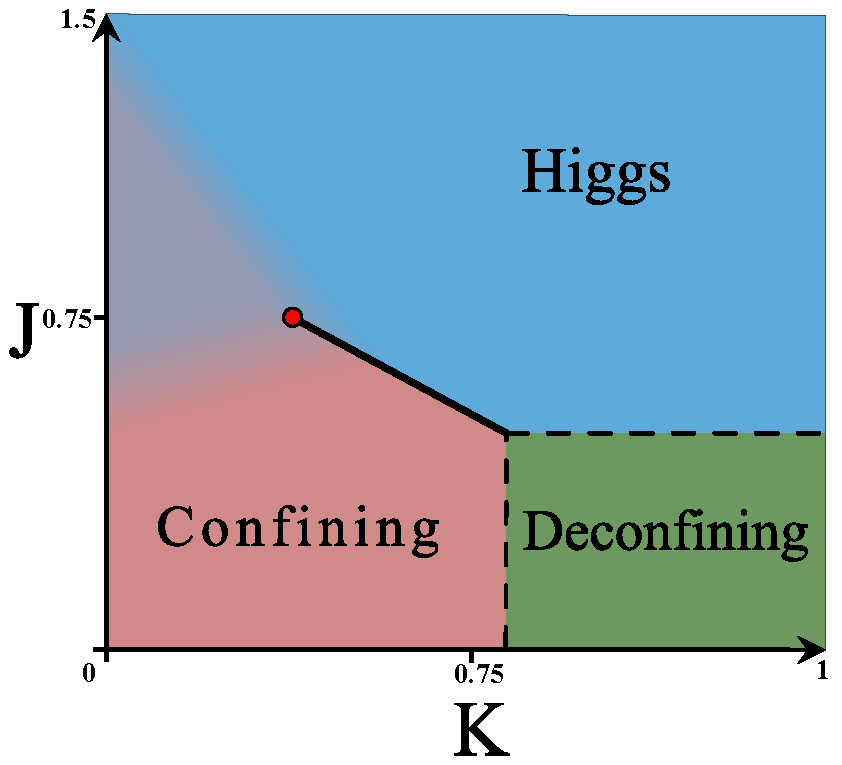
\includegraphics[width=.42\textwidth]{figures/chapter2/Z2Z2phasedia.pdf}%
	\raisebox{-.13in}{
		\includegraphics[width=.45\textwidth]{figures/chapter2/Z2Z2.pdf}}
	\caption{The quantitative phase diagram as established by Monte-Carlo of the $Z_2 / Z_2$ theory as function of the gauge coupling $K$ and matter coupling $J$, see appendix \ref{app:mc-details} for details. The left panel gives the overview, further illustrated by  the outcomes for the specific heat in the right panel. The dashed- and drawn lines represent second- and first order transitions respectively, that we confirmed by a detailed analysis of the Binder cumulants. This is well understood (see main text): for small $J$ the matter sector is disordered and can be ignored, and one is just dealing with the pure gauge Wegner Ising gauge theory revealing the deconfining- and confining phases separated by a continuous phase transition, where the latter can be viewed as a condensate of gauge fluxes (``visons''). Upon increasing $J$ at  large $K$ one enters the ``Higgs-like'' phase that is famously indistinguishable from the confining phase -- a transition is absent as function of $J$ for small $K$. A peculiarity is the first order line emanating at the tricritical point anchored at the deconfinement transition. This reflects a van der Waals density driven liquid-vapor transition associated with the density of ``featureless'' domain walls, terminating at a critical end point.}
	\label{Z2Z2phasediagram}
\end{figure*}

\section{ A short review of $Z_2$ gauge theory with matter.}
\label{Z2Z2review} 

Let us first remind the reader of the thorough understanding of Wegner Ising gauge theory, both for matter in the fundamental ($Z_2$) and the  case of matter fields with a larger symmetry than the fundamental. The pure gauge theory played a decisive role in the very early days of Yang-Mills theory by demonstrating the existence of confining/deconfining phase transitions \cite{Wegner} in 3 and higher (overall) dimensions, highlighted by the famous lecture notes  by Kogut \cite{Kogut}. Among others, the pure $Z_2$ gauge is dual to global Ising, while the deconfining phase was much later understood as being characterized by topological order. For a particularly appealing physical interpretation see the ``stripe fractionalization'' \cite{stripefrac,stripefracdemler}. 

The essence is the invariance of the theory Eq. \eqref{eq:z2action}  under the local gauge transformations at each site $i$, 
\begin{eqnarray}
	\ket{\text{state}} &\rightarrow  &\prod_j \sigma_{ij}^x \ket{\text{state}} \nonumber \\
	\phi_i^a &\rightarrow  & -\phi_i^a \mathperiod
	\label{gaugetrans}	
\end{eqnarray}
The bond variables are Ising valued $(\pm1)$ and the action is invariant under flipping the signs of all bonds emanating from any site $i$ when simultaneously the matter (vector) fields living on the site revers their signs. For vanishing (and by extension small) matter couplings $J_a$ one is in the realms of the pure gauge theory (see Fig.\ref{Z2Z2phasediagram}). This is best understood in terms of the topological excitations, the ``gauge fluxes'' \cite{Kogut} also called ``visons'' in the condensed matter literature \cite{visons}. The gauge invariant object is the $Z_2$ valued Wilson plaquette variable $\tau^z_{12}\tau^z_{23}\tau^z_{34}\tau^z_{41}$: for an even or uneven number of positive bond variables $\tau^z_{ij}$ this takes a positive or negative value, the latter representing gapped excitations when $K$ is large. 

\begin{figure*}[!h]
	\centering
	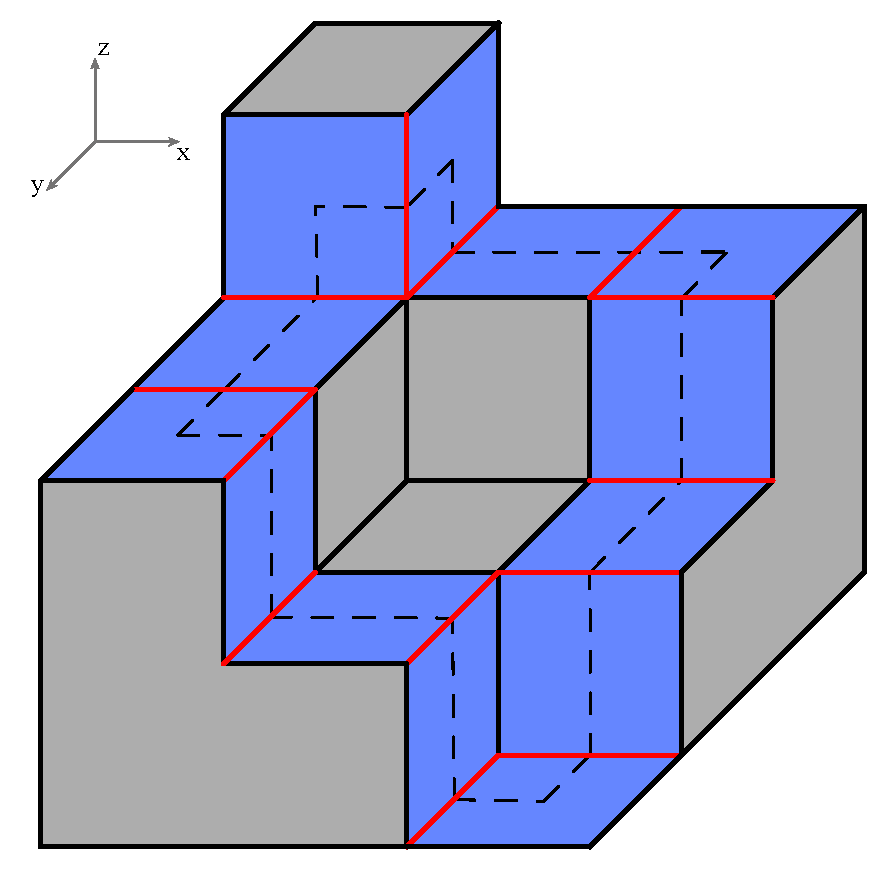
\includegraphics[scale=.5]{figures/chapter2/Looptopil.pdf}
	\caption{An example of a closed $Z_2$ gauge flux (``vison'') loop as these occur in the deconfining (and Higgs ``like'') phase representing the topological excitation of the gauge theory. The plaquettes indicated by blue represent a gauge invariant  flux $\tau^z_{12}\tau^z_{23}\tau^z_{34}\tau^z_{41} = -1$ immersed in a background of positive plaquette values. These have to form a connected line in three dimensions, the dashed line in this illustration. } 
	\label{loopexample}
\end{figure*} 


These visons have a similar status as the monopoles of compact QED \cite{PolyakovQED}, the difference being that these fluxes have co-dimension $d-2$: in 3 dimensions these correspond with ``world lines'' (see Fig. \ref{loopexample}). It is easy to see that a Dirac seam emanates from the line (forming a surface) and for large $K$ these form small closed loops protecting the topological order. As for global $U(1)$ in 3D, upon reducing $K$ these loops grow in size to ``blow out'' at the transition to the confining phase that can be viewed as a condensate of the ``vison particles''. It is easy to demonstrate \cite{Kogut} that the (gauge invariant) Wilson loop exhibits a perimeter law when the visons are expelled from the vacuum (deconfinement), turning into an area law in the confining phase (vison condensate). This explains the small $J$ regime of all phase diagrams that we will present. 

\begin{figure*}[!h]
	\centering
	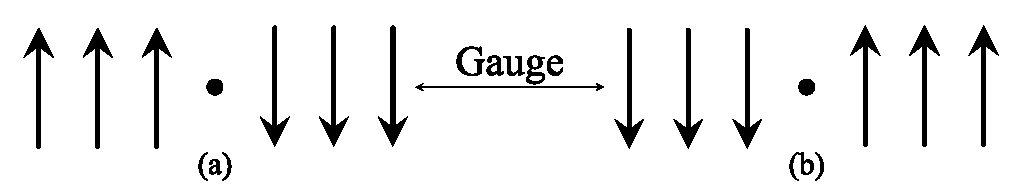
\includegraphics[scale=.4]{figures/chapter2/Z2Z2domainWall.pdf}
	\caption{The featureless nature of the Higgs ``phase'' of the $Z_2/Z_2$ theory explained by inspecting the domain walls in the large $J,K$ regime. Depart from the unitary gauge (upper row) and construct a domain wall costing an energy $J$/unit cell. Restore the gauge invariance implying that on every site an up spin cannot be distinguished from a down spin. This shows that  the domain wall has the gauge invariant meaning of an object carrying energy but nothing else. This is the crucial insight behind the indistinguishability of the Higgs and confining phases.}
	\label{Z2Z2domainwall}
\end{figure*} 


Let us now turn on the matter couplings $J^a$ to focus in on the case of minimal $Z_2$ matter ``in the fundamental''. As we already emphasized, the demonstration by Fradkin and Shenker \cite{Fradkinshenker} that the ``maximally orderly'' and ``maximally disorderly'' Higgs and confining phases are actually indistinguishable caused initially confusion. But in hindsight it is obvious, for the simple reason that a phase transition requires a {\em global}, gauge invariant symmetry to be broken. But in the presence of single $Z_2$ matter, global symmetry is erased. Consider the large $K,J$ limit; the visons are completely expelled and one can choose a unitary gauge fix taking all bond variables to be positive and the matter field living on the sites form an ordered Ising state with the spins, say, pointing up. However, according  the gauge transformation Eq. (\ref{gaugetrans}) on every site this can be swapped to a down spin. This sense of Ising order has no gauge invariant meaning and a global symmetry that is broken cannot be identified, and thereby there is no distinction from the confining phase. 

From tracking parameters along the large $J$ limit varying $K$ followed by descending along $J$ for small K one finds no phase transition proving the indistinguishability of the Higgs and confining phases. The oddity is however in the form of a ``strand'' of first order transitions emanating from the tricritical point anchored at the pure gauge confining-deconfining transition; the deconfining phase keeps of course its identity characterized by the expelled visons. This will be an important motif in the remainder: it is a peculiarity of the ``amplitude sector'' of  these gauge theories, that was elucidated by Huse and Leibler in a particularly appealing physical setting \cite{HuseLeibler}. 


Although there is no manifest global symmetry, there is a ``material dynamics'' at work that becomes obvious considering the topological excitations, see Fig. \ref{Z2Z2domainwall}.  It is instructive to depart from the large $K,J$ limit. Consider the unitary gauge fix where one is dealing with a standard Ising model, characterized by domain walls as topological excitation costing an energy  $E \sim J$/unit cell. However, upon restoring gauge invariance it ``looses the symmetry'': for instance one can swap all spins to the left of the domain wall from up to down and the other way around to the right. Although the matter spins ``disappear'', the presence of the domain wall as en energetic excitation is a gauge invariant notion. This is the simple clue; upon reducing $J$ such featureless domain walls will start to proliferate.  

Let us now decrease $K$ such that (closed) vison loops start to form. It is easy to find out that the $Z_2/Z_2$ domain walls and visons relate to each other in the same way as the (Abrikosov) flux lines and magnetic monopoles of the compact $U(1)/U(1)$ theory, where the monopole ``cuts open'' the flux line. The vison loop ``cuts open'' the domain wall surface. For small $J$ and large $K$  in the ``Higgs like'' phase one finds accordingly large domain wall surfaces  with here and there a small hole (``vesicles'' \cite{HuseLeibler} ). However, for small $K$ and finite $J$ (``confinement like'') there are many visons  and accordingly the domain walls are ``cut in small pieces'' (``platelets''  \cite{HuseLeibler}).  

This offers the crucial insight regarding the origin of the first order line separating the confining and Higgs like regime. The net density of domain walls takes the role of density in the van der Waals theory dealing with liquid-vapor transitions. This is just the ubiquitous affair where the density changes discontinuous in a first order transition in the pressure-temperature diagram, terminating at a critical point. Huse and Leibler argue that this particular ``platelet'' versus ``vesicle'' incarnation is literally related to the behaviour of lipid membranes as of great relevance to e.g. biology\cite{HuseLeibler}. One take-home message of our work is that this peculiar ``amplitude dynamics'' is surprisingly ubiquitous in the whole landscape of theories defined by Eq. (\ref{eq:z2action}). 

The next general motif that will be important is associated with matter field characterized by a larger symmetry than the gauge sector. In general, this will imply that a gauge invariant {\em global} symmetry can be identified, that is broken in the Higgs phase, restoring the distinguishability with the confining phase. The simplest example is the single copy $O(N)/Z_2$ system. 

This ``left over'' global symmetry breaking is easy to infer in the large $K,J$ limit. In unitary gauge one finds here an ordered state breaking the $O(N)$ symmetry. However, the gauge transformation transforms the vector into minus itself. Consider $O(3)$ in 3D: this turns the vector in the {\em director} order parameter of a {\em uniaxial nematic}. The confinement-Higgs transition becomes in turn equivalent to the liquid crystal nematic-isotropic transition. This was used by Toner et al. \cite{toner95} to shed light on the origin of the well known first order character of this transition. One way is to consider small $K$ to integrate out perturbatively the gauge fluctuations, the outcome being that one recovers the Landau-de-Gennes theory governed by a rank two traceless symmetric tensor order parameter, allowing for a cubic invariant responsible for the first order transition. However, the dual (topological) language elucidates that {\em two} global symmetries are now simultaneously broken by the vison condensation as well as the manifest nematic order. We notice that this gauge theory strategy was used recently to completely classify and study ``generalized nematics''  associated with the breaking of rotational symmetry to any of the (non-Abelian) three dimensional point groups. This is a remarkably rich affair, with the highly symmetric point groups translating in high rank tensor order parameters \cite{nonabnematic,nonabnematic1,nonabnematic2}.

\begin{figure*}[!h]
	\centering	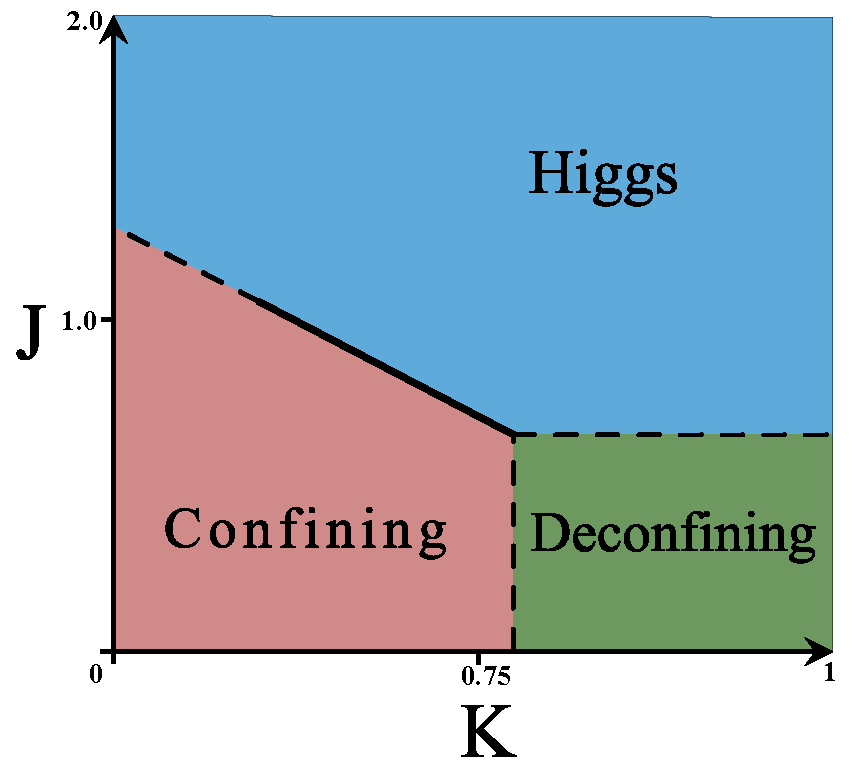
\includegraphics[width=0.425\textwidth]{figures/chapter2/O2Z2phasedia.pdf}
	\raisebox{-.13in}{
		\includegraphics[width=0.44\textwidth]{figures/chapter2/O2Z2.pdf}}
	\caption{In the left panel the phase diagram of the $O(2)/Z_2$ theory, established from the Monte Carlo results for the specific heat $c_V$ in the right panel. This can be directly compared with the $Z_2/Z_2$ theory, Fig.\ref{Z2Z2phasediagram}. One infers that it looks very similar, the only difference being that now the ``gap'' between the termination of the first order line and the $K \rightarrow 0$ limit between the confining- and Higgs phase is now interrupted by a second order phase transition associated with the breaking of the gauge invariant ``half-periodic'' $O(2)$ symmetry. The fact that in other regards the phase diagrams look so similar is surprising, see the main text. } 
	\label{O2Z2phasediagram}
\end{figure*}



A final motif that will be useful in the remainder is associated with the ``outlier'' Abelian matter $O(2)/Z_2$ case that is also well known, especially in the context of ``fractionalized'' superconductivity (e.g., \cite{visons}).  Different from the non-Abelian $O(N)$ cases in the small K limit the rank two tensor order parameter simplifies to a simple $O(2)$ with halved periodicity, 
\begin{equation}
	H_{\mathrm{eff}, K \rightarrow 0} = -J' \sum_{\langle i, j \rangle} \left( \vec{\Phi}_i \cdot \vec{\Phi}_j \right)^2  = -J' |\Phi|^2 \sum_{\langle i, j \rangle} \cos \left( 2 (\phi_j - \phi_i ) \right) ~,
	\label{directorH}
\end{equation}         
using $\vec{\Phi}_i = |\Phi | e^{i \phi_i}$. This has the obvious ramification that for $K \rightarrow 0$ this transition continues to be second order.  In Fig.\ref{O2Z2phasediagram} we show the phase diagram. There is now indeed a second order transition separating the Higgs and confining phases, associated with the disappearance of the ``halved periodicity'' XY order parameter characterizing the Higgs phase. However, upon increasing $K$ this turns into a first order line again. Strikingly, this first order ``strand'' is even quantitatively very similar as its analogue in the $Z_2/Z_2$ case: the main difference is just that the ``connection'' between confining and Higgs is now closed off by the transition involving the manifest XY order parameter.  This is clearly associated with the amplitude of the order parameter that obviously submits to the same ``Huse-Leibler'' logic, being controlled by the density of the ``non-topological'' matter defect ``fragments'' near the tricritical point. 

Although it has been previously observed that close to the tricritical point the Higgs-confinement transition has turned first order \cite{Senthil} it took us by surprise that the $O(2)/Z_2$ behavior behaves so similarly as to the $Z_2/Z_2$ case: the only essential difference is that the ``gap'' between the critical end point and the $K \rightarrow 0$ limit is just ``filled'' with the nematic-to-isotropic like second order transition, barely affecting even the locus of the end point of the first order line. A priori it is not at all obvious why this is so similar. For instance, the matter topological excitations, as identified in unitary gauge, are now XY-vortices with a quantized rotation associated with the halved periodicity. These are lines (and not surfaces) in 3D, in stark contrast with the Ising domain walls of the $Z_2/Z_2$ theory. We will encounter underneath other variations on this theme, invariably revealing this somewhat mysterious quantitative universality of the Huse-Leibler motif.     

\section{Replicating the $Z_2$ matter fields: two copies.}
\label{replZ2}

After these preliminaries let us now turn to the main subject: the family of ``replicated'' Ising gauge theories. The simplest case is the $Z_2$ matter theory with two matter copies:  $Z_2 \times Z_2 / Z_2$. In fact, the most interesting  case is the truly minimal one where we take the same matter field coupling $J_1 = J_2 = J$ and set the local couplings to zero $J^{12}_L = 0$. Under these circumstances the matter fields couple only through the Ising gauge fields.  

Let us start with the simplest example of a $Z_2$ gauge theory with replicated matter: the $Z_2 \times Z_2 / Z_2$ case. In Fig.\ref{Z2xZ2Z2phasediagram} we show the phase diagram as established by our Monte-Carlo simulations.  We infer that this is a very close sibling of the $O(2)/Z_2$ phase diagram that we just discussed Fig.\ref{O2Z2phasediagram}. Next to the ubiquitous Higgs-deconfining transition, the transitions between the Higgs- and confining phase looks very similar, including the first order line emanating from the tricritical point turning second order roughly at the locus of the $Z_2/Z_2$ critical endpoint. 

\begin{figure*}[!h]
	\centering	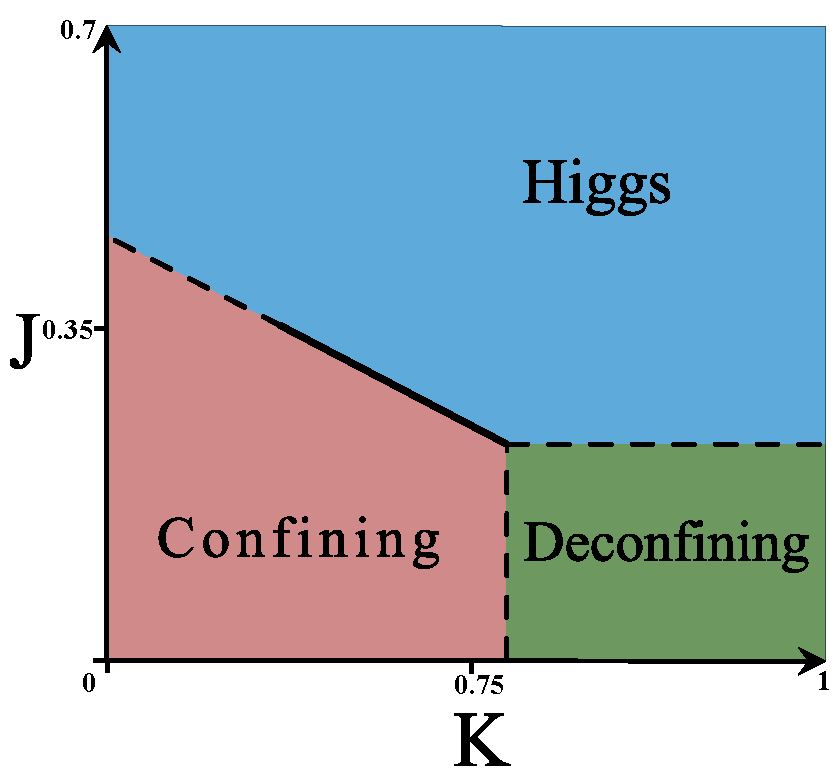
\includegraphics[width=0.425\linewidth]{figures/chapter2/Z2xZ2Z2phasedia.pdf}
	\raisebox{-.13in}{
		\includegraphics[width=0.44\linewidth]{figures/chapter2/Z2xZ2Z2.pdf}}
	\caption{ The phase diagram of the ``two copy''  $Z_2 \cross Z_2 / Z_2$ theory for $J_1 = J_2  = J$ and $J_L^{12} = 0 $ illustrated by  the Monte Carlo results  for the specific heat $c_V$ in the right panel. This looks very similar as to the $O(2)/Z_2$ case (Fig.\ref{O2Z2phasediagram}) in turn similar to the $Z_2/Z_2$ case  except for the connection between Higgs- and confinement is closed off by an honest second order transition. As explained in the text, one can now identify an Ising valued gauge invariant ``registry'' order parameter that breaks the symmetry spontaneously in the Higgs phase having a similar role as the nematic order parameter of the $O(2)/Z_2$ case.} 
	\label{Z2xZ2Z2phasediagram}
\end{figure*}

What is going on here? As explained earlier, for the transition between confining and Higgs at low $K$ to be a true second order phase transition, there has to be a broken global symmetry. In fact this is indeed controlled by a gauge invariant order parameter with a global Ising symmetry that may not be directly obvious to the reader, but it is quite simple. Consider again the unitary gauge with all bond spins $+ 1$. Because we have two matter fields, we are now dealing with two {\em independent} Ising spin systems living on the sites that will both be ordered for large $J,K$. As we emphasized in Section \ref{Z2Z2review}, after restoring the gauge invariance  both Ising spin systems ``loose their symmetry'' according to the $Z_2/Z_2$ rule book. But now we observe that the relative orientation of these two spin systems actually corresponds  with a  gauge invariant, global $Z_2$ symmetry! 

\begin{figure*}[!h]
	\centering
	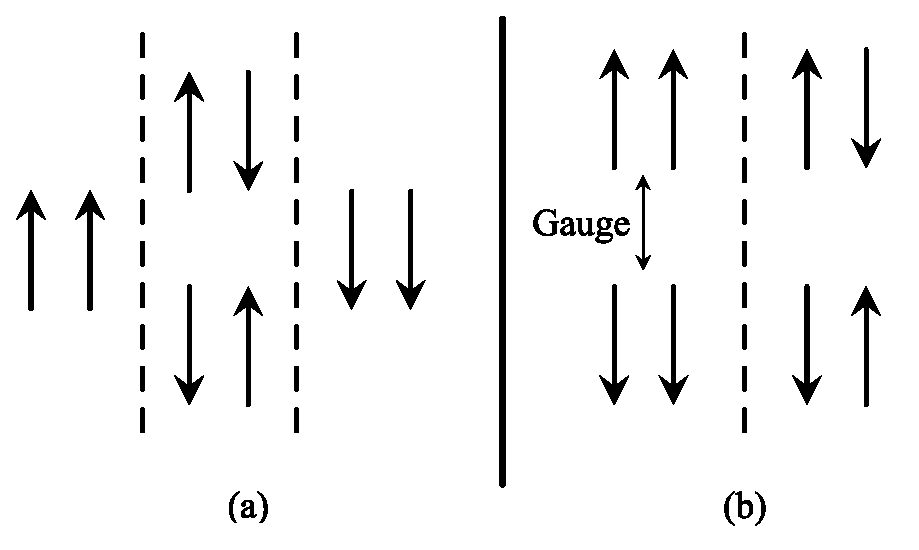
\includegraphics[scale=.4]{figures/chapter2/Z2xZ2Z2domainWall.pdf}
	\caption{The ``registry'' order parameter of the two copy $Z_2 \times Z_2/Z_2$ theory. Depart from the large $J,K$ limit and take a unitary gauge fix as in Fig.\ref{Z2Z2domainwall}. One can now construct two types of domain walls associated with the two copies (upper line). However, upon restoring gauge invariance only two of the four on-site configurations can be distinguished: the spins are locally either parallel- or anti-parallel.  This is the global $Z_2$ symmetry that is broken in the Higgs phase.} 
	\label{twocopyregistry}
\end{figure*} 

Take the matter spins ``1'' to be pointing in the positive direction, and the ``2'' spins can be either parallel or anti-parallel to the ``1'' spins. Let us now see what happens with this ``registry'' upon restoring the gauge invariance, see Fig.\ref{twocopyregistry}. Consider parallel registry on a particular site like  $ \uparrow_{1} \uparrow_{2}$ and  under a gauge transformation both spins flip -- a single sector $\uparrow, \downarrow$ is not  gauge invariant. But it follows that the {\em relative} orientation of the matter spins in both sectors can be either {\em parallel} or {\em anti-parallel} and after restoring the gauge invariance it continues to be distinguishable whether one is dealing with locally parallel or anti-parallel configurations:  $ \downarrow_{1} \downarrow_{2} \leftrightarrow \uparrow_{1} \uparrow_{2}$ versus $ \uparrow_{1} \downarrow_{2} \leftrightarrow \downarrow_{1} \uparrow_{2}$! This is what we call the ``registry order parameter'' which carries clearly a global $Z_2$ charge!

This ``registry'' symmetry breaks spontaneously in the Higgs phase, causing a two fold degenerate ground state: either the ``parallel'' or ``anti-parallel'' registry takes over. This registry order parameter $\langle \phi^1\phi^2\rangle$ is easy to measure and it is precisely what we find in the Monte-Carlo simulation of the Higgs phase, see Fig.\ref{Z2xZ2Z2orderParameter}.
\begin{figure*}[!h]
	\centering
	\includegraphics[scale=.7]{figures/chapter2/orderParameterZ2xZ2Z2K0.pdf}
	\caption{Expectation value of the registry order parameter $\langle \phi^1\phi^2\rangle$ of the  $Z_2 \times Z_2 / Z_2$ theory, along the $K=0$ slice.} 
	\label{Z2xZ2Z2orderParameter}
\end{figure*}

At first sight this may be a bit confusing given that the matter fields interact only via the gauge couplings. However, the simple logic in the previous paragraph just reveals that this replicated system has in the Higgs phase a doubly degenerate ground state associated with ``parallel'' and ``anti-parallel'' registry. It is easy to construct gauge invariant domain walls between domains with opposite registry, as the ``featureless'' domain walls of the $Z_2/Z_2$ theory now acquire the gauge invariant meaning that they represent a jump in the registry order. Notice that the phase diagram is in all regards other than the second order  Higgs-confinement transition a near quantitative copy of the $Z_2/Z_2$ phase diagram. Given the lessons of the $O(2)/Z_2$ theory this is perhaps not surprising since the ``microscopy'' of the $Z_2 \times Z_2 / Z_2$ theory is a close cousin of the  $O(2)/Z_2$ case.  

\begin{figure*}[!h]
	\centering
	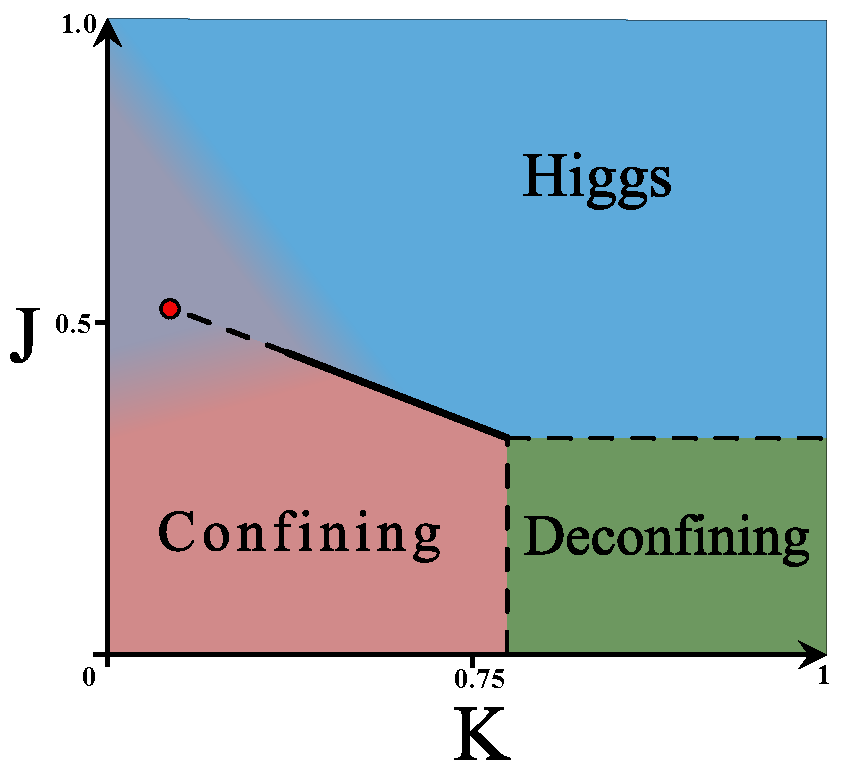
\includegraphics[width=.32\textwidth]{figures/chapter2/Z2Z2Jl01phasedia.pdf}
	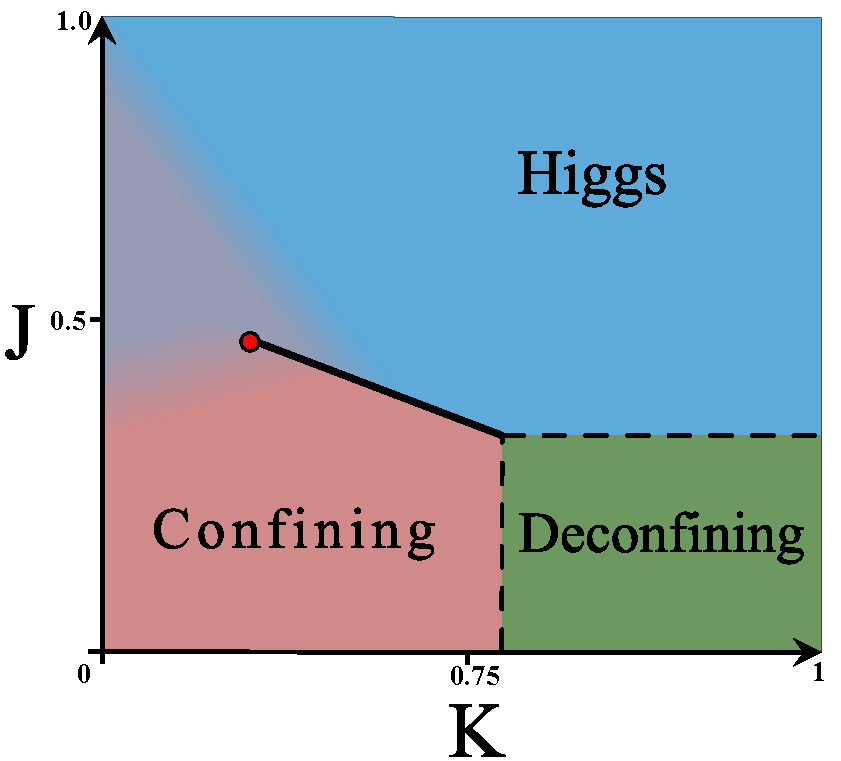
\includegraphics[width=.32\textwidth]{figures/chapter2/Z2Z2Jl1phasedia.pdf}
	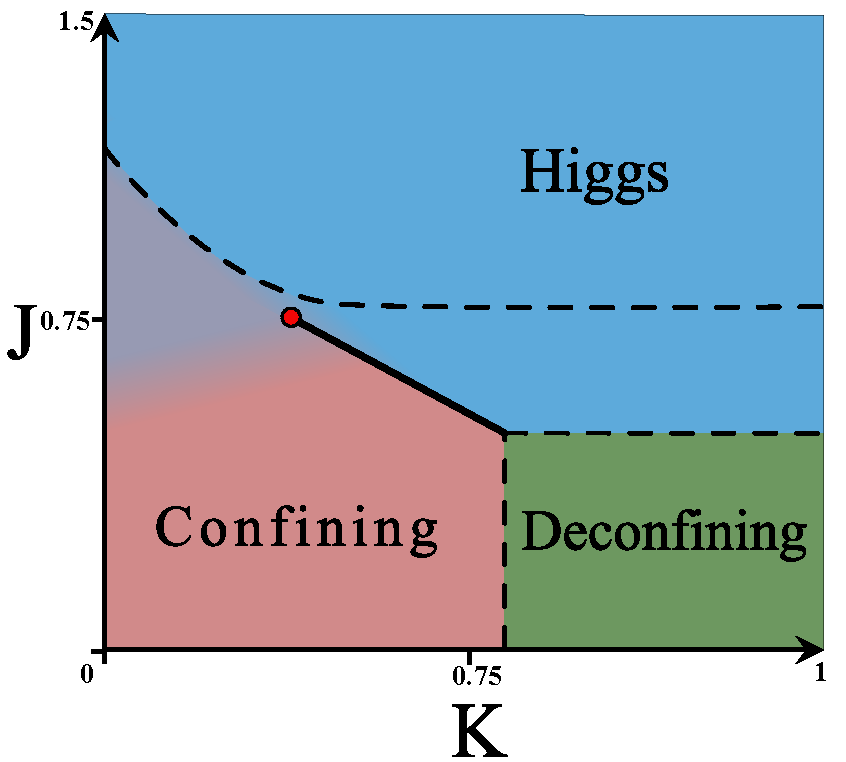
\includegraphics[width=.32\textwidth]{figures/chapter2/Z2Z2diffJphasedia.pdf}\\
	\raisebox{-.1in}{	\includegraphics[width=.32\textwidth]{figures/chapter2/Z2xZ2Z2_gap_01.pdf}}
	\hfill
	\raisebox{-.1in}{
		\includegraphics[width=.32\textwidth]{figures/chapter2/Z2xZ2Z2_gap_1.pdf}}
	\hfill
	\raisebox{-.1in}{	\includegraphics[width=.32\textwidth]{figures/chapter2/Z2xZ2Z2_2J.pdf}}
	\\		
	\caption{The phase diagrams of the $Z_2 \cross Z_2 / Z_2$ theory, with the Monte Carlo data for $c_V$ in the second row, for a finite  $J_L=0.1$ (\textbf{a}) and $J_L = 1$ (\textbf{b}). Notice that  the Monte Carlo results are shown over a small interval in $K$ to highlight the most relevant changes.  This local  coupling acts as a field breaking the registry symmetry explicitly, turning the $J_L =0$ Ising phase transition into a cross over. The consequence is that for any finite $J_L$ the indistinguishability of Higgs and confinement is restored. The small strand of second-order like (dashed line) transition for  small $J_L$ (\textbf{a}) may well be related to a rapid crossover that can not be distinguished within our numerical accuracy (Binder criterium) from a real transition. For large $J_L$ (\textbf{b}) the phase diagram becomes nearly identical to the one of the $Z_2/Z_2$ theory itself. Another interesting game is to vary the relative strength of the matter coupling of the two copies for $J_L =0$.  In (\textbf{c}) we show a typical example  dealing with different matter couplings $J = J_1 = 3 J_2$.}
	\label{Z2xZ2Z2Jl}
\end{figure*}

To illustrate these matters further, let us consider what happens when the local $J_L^{12}$ interaction in Eq. (\ref{eq:z2action}) is switched on. It is immediately obvious that this relates directly to the registry: one sees immediately departing from unitary gauge that this lifts the degeneracy of the parallel and anti-parallel registry configurations. This acts as a field breaking the registry Ising symmetry explicitly! This should have the effect to turn the registry phase transition into a cross over, with the effect that yet again the confining and Higgs phases become indistinguishable again, and this is what we find is going on according to our MC simulations: see Fig.\ref{Z2xZ2Z2Jl}  (\textbf{a},\textbf{b}). 

A next freedom one can exploit is to take $J_L =0$ but change instead the relative magnitude of the matter couplings, $J = J_1 \neq J_2$.  This is an entertaining affair highlighting the unusual nature of the registry order. Upon reducing $J_2$ the locus on the vertical axis where this second field changes from order to disorder shifts upwards along the vertical axis in terms of the ``dominating'' copy governed by $J_1=J$. The effect is that at the $J_1$ transition in the small $K$ regime the $J_2$ coupled matter field is still {\em disordered} 
while the order in both fields is required for the existence of the registry order! Hence, holding $J_1\neq J_2$ fixed while varying $K$, there is a window where the registry order disappears in the small $K$ regime, switching on again when $K$ has become sufficiently large to reach the $J$ where also the second field becomes also prone to order again, see Fig.\ref{Z2xZ2Z2Jl}(\textbf{c}). The outcome is a critical end point where now a line of second order transitions starts that is subsequently turned into the first order Huse-Leibler affair! We notice that this peculiar behaviour is only seen in a small $J_2/J_1$ interval; for $J_2 \le 0.25 J$ the phase diagram becomes again the one of the single copy $Z_2/Z_2$ theory.

\bigskip

Up to this point we have demonstrated that in terms of the degrees of freedom of the gauge theory a quantity can be identified characterized by a global symmetry that is broken in the Higgs phase -- the registry order parameter. However, what is the nature of the {\em dynamics} responsible for the stability of this order? Inspecting this deep in the Higgs phase (large $K,J$) employing the unitary gauge is not informative. The reason is that this is rooted in ``gauge field interactions'' that are unusual   in the sense that the discrete nature of the $Z_2$ gauge fields implies that these ``gauge forces'' are characterized by a mass scale that becomes large deep in the Higgs phase. In a statistical physics language any gauge field mediated force may be viewed as an ``order-out-of disorder'' phenomenon -- the fluctuations of the gauge fields are responsible for the interactions between the (gauge invariant) matter fields. 

Hence, the limit to consider is $K=0$: the visons are the dynamical degrees of freedom of the discrete gauge theory and these come for free in this limit. Given that the disclinations are bound states of matter defects (domain walls) and the visons, the stability of the Higgs phase itself is entirely due to the cost associated with the former, while the $Z_2$ gauge field is maximally fluctuating. Its only energy cost comes from the coupling to the matter fields. The gauge fields can therefore be straightforwardly integrated out with the outcome that one obtains the (gauge invariant)  Landau-de-Gennes order parameter theory \cite{toner95}. In the general case one is dealing with the point groups associated with the rotational symmetry of the nematic-type state; for Abelian point groups in two dimensions that are encoded by $Z_N$ gauge fields one recovers in this way the simple ``p-adic'' nematics \cite{nematic2D}, while this procedure has been shown to be instrumental to derive the high rank tensor de-Gennes order parameters associated with the non-Abelian point groups in three dimensions \cite{nonabnematic,nonabnematic1,nonabnematic2}. 

The outcome for the elementary $Z_2$ gauge theory is simple: integrating out the gauge fields when $K=0$ leads to the simple ``square of the Hamiltonian'' gauge invariant effective theory as in Eq. (\ref{directorH}) \cite{toner95}. In full generality, departing from the replicated theory with arbitrary matter field symmetry Eq. (\ref{eq:z2action}) when $J_L^{ij} =0$ and all $J_i = J$ one obtains, 
\begin{equation}
	H_{\mathrm{eff}, K =0, } = -J' \sum_{\langle i, j \rangle} \left( \sum_{a=1}^{N_\text{rep} } \vec{\phi}_i^a  \cdot \vec{\phi}_j^a \right)^2 ~.
	\label{Z2deGennes}
\end{equation}
Let us first consider the single replica $Z_2$ matter field. Here $\vec{\phi_i} \rightarrow \sigma^z_i$ and we infer that the effective Hamiltonian becomes $\sum_{\langle i, j \rangle} (\sigma^z_i \sigma^z_j ) ^2 \rightarrow \mathrm{constant}$: this is the essence of the Fradkin-Shenker observation \cite{Fradkinshenker}, no gauge invariant degree of freedom can be identified distinguishing the Higgs and confining phases implying that these are indistinghuishable. But let us now consider two identical $Z_2$ copies,
\begin{equation}
	\begin{split}
		H_{\mathrm{eff}, K =0, N_{\text{rep}} = 2} &= -J' \sum_{\langle i, j \rangle} \left( \sum_{a=1}^{2} (\sigma^z)_i^a  \cdot (\sigma^z)_j^a \right)^2 \\ &= 
		\mathrm{constant} - J'  \sum_{\langle i, j \rangle} \left( (\sigma^z)_i^{(1)} ( \sigma^z)_i^{(2)} \right) \left( ( \sigma^z)_j^{(1)} (\sigma^z)_j^{(2)} \right) \mathperiod
	\end{split}
	\label{twocopyZ2deGennes}
\end{equation}
This simple affair reveals the origin of the ``registry dynamics'': the combination $\left( (\sigma^z)_i^{(1)} (\sigma^z)_i^{(2)} \right)$ takes the (global) $Z_2$ values $ \pm 1$ for parallel and anti-parallel registry and Eq. (\ref{twocopyZ2deGennes}) is just an Ising Hamiltonian associated with the registry degrees of freedom.

In hindsight this is elementary. As for the uniaxial nematics of Toner {\em et al.} \cite{toner95}, the gauge theory in the strong coupling regime ($K \rightarrow 0$) is in fact a redundant parametrization of the ``director'' gauge invariant de Gennes type theories. The additional richness of the gauge theory is associated with $K$ becoming large, i.e. the weak coupling regime of the gauge theory. For instance, the topologically ordered {\em deconfining} phase has no physical identification dealing with the ``molecular'' nematic liquid crystals. Additional microscopic structure is required, with perhaps the ``stripe fractionalization'' \cite{stripefrac,stripefracdemler} being the most elementary example of how this can happen. 

This is also underlying the difficulty to recognize this simple  motif ``deep'' in the Higgs phase, for large $J$ and $K \rightarrow \infty$. Departing from the unitary gauge one easily identifies the registry as gauge invariant degree of freedom (as in the above) but at first sight the dynamics stabilizing it is obscure. The reason is of course that the visons are now highly energetic excitations  requiring an energy $E\sim K$ per unit length associated with the effect that the gauge symmetry is discrete and the gauge fields are massive . However, there is no phase transition in the Higgs phase at large $J$, varying $K$ from zero to infinity. This implies that regardless the magnitude of the virtual visons their fluctuations {\em always} suffice to hard wire the registry order. This may be viewed as an order-out-of-disorder phenomenon pushed to its extreme.  



\section{The case of many  $Z_2$ matter fields.}
\label{replmanyZ2}

Having established the rules for two $Z_2$ matter fields copies, how does this generalize to many copies? Let us depart again from Eq.(\ref{eq:z2action}) for $Z_2$ matter and consider an arbitrary number of matter field copies $N_{\text{rep}}$. As before the circumstances optimal for the registry type order are associated with setting all local couplings to vanish, $J_L^{ab} = 0$, and taking the matter fields couplings to be equal: $J_a = J$. It is in fact easy to find out by induction how the registry spontaneous symmetry breaking of the two copy case generalizes to many copies.




Let us consider the three copy case:  $Z_2 \times Z_2 \times Z_2/ Z_2$. We just proceed as before, departing from deep in the Higgs phase (large $K,J$) and using the unitary gauge. At every site the matter fields can occur in $2^3$ different configurations, see  Fig.\ref{threecopyexample}. Identifying these with domains one would find accordingly 8 different domain walls associated with flipping one spin keeping the other spins fixed. However, upon restoring the gauge invariance amounting to flipping {\em all} spins on the site, it follows that configurations are pairwise associated, e.g.  $\uparrow \uparrow \uparrow \leftrightarrow  \downarrow \downarrow \downarrow$. Accordingly, one finds 4 distinct gauge invariant vacuum states, separated by ``single spin'' domain walls. This is governed by a $p = 4$ state {\em Potts model}! It is easy to check that the Ising registry theory Eq.(\ref{twocopyZ2deGennes}) generalizes to the 4-state Potts theory  by considering the ``squared'' de-Gennes type effective theory in the $K \rightarrow 0$ limit. 

\begin{figure*}[!h]
	\centering
	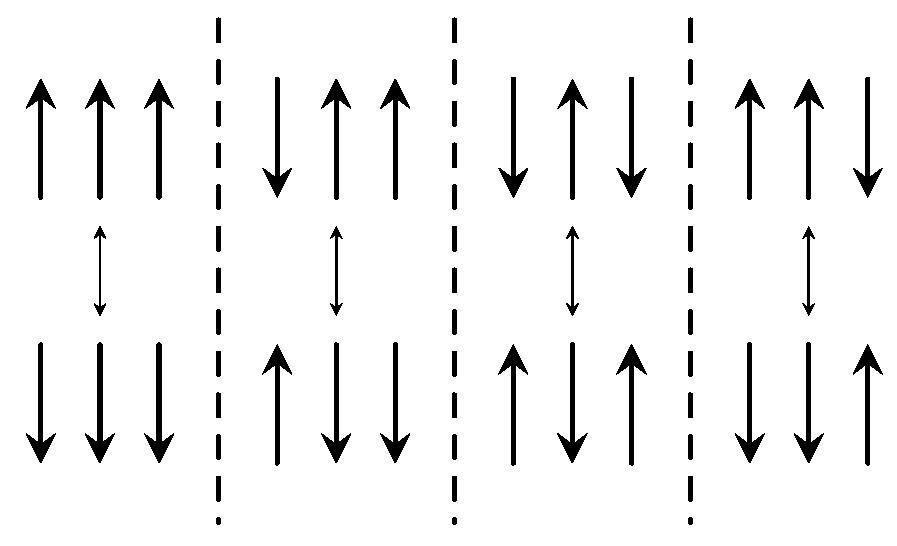
\includegraphics[scale=.4]{figures/chapter2/Z2xZ2xZ2Z2domainWall.pdf}
	\caption{The registry order parameter (see main text) in the case of the three copy $Z_2 \times Z_2 \times Z_2/Z_2$ theory. Depart from unitary gauge fix and the three matter fields can locally form eight configurations. However, under gauge transformations half of them are redundant, e.g. $\uparrow \uparrow \uparrow \leftrightarrow \downarrow \downarrow \downarrow$. The gauge invariant registry order parameter takes therefore four different physical realizations and it is governed by a $p=4$ state Potts model.}
	\label{threecopyexample}
\end{figure*} 


\begin{figure*}[!h]
	\centering	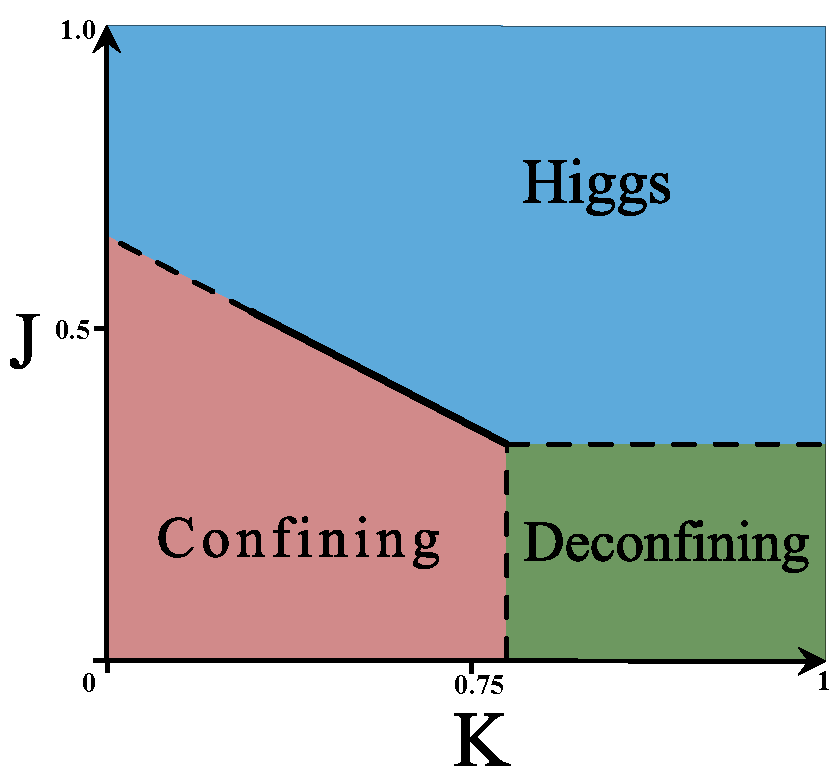
\includegraphics[width=0.425\textwidth]{figures/chapter2/Z2xZ2xZ2Z2phasedia.pdf}
	\raisebox{-.13in}{
		\includegraphics[width=0.45\textwidth]{figures/chapter2/Z2xZ2xZ2Z2.pdf}}
	\caption{The phase diagram of the three copy $Z_2 \cross Z_2  \cross Z_2/ Z_2$ theory as in Fig.\ref{Z2Z2phasediagram} and Fig.\ref{O2Z2phasediagram} for the ``minimal'' $J_a =J$ and $J^L_{ab} = 0 $ case. This looks very similar to Fig.\ref{Z2xZ2Z2phasediagram} and the strand of the first order transitions is barely changed. The specific heat $c_V$ data suggests a first order transition all the way down to $K=0$, but a Binder cumulant study reveals this change to second order as sketched. A major distinction now is that dynamics of (continuous) confining to Higgs transition is governed by a $p=4$ state \textit{Potts model}.} 
	\label{Z2xZ2xZ2Z2phasediagram}
\end{figure*} 

This is confirmed by our MC simulations. In Fig.\ref{Z2xZ2xZ2Z2phasediagram} we show the phase diagram of the three copy model. As anticipated, this looks very similar as to the two  copy case, Fig.\ref{Z2xZ2Z2phasediagram}. Although the dynamics is quite different --- the 4 distinct ``gauged'' domain walls associated with $p=4$ Potts --- the Huse-Leibler first order strand is barely affected with yet again the registry order being responsible for the continuous (Potts model) phase transition distinguishing the confining and Higgs phases. In Fig.\ref{Z2xZ2xZ2Z2snapshot} we show a typical  realization after a partially annealed Monte-Carlo ``quench'' deep in the Higgs phase: one discerns the 4 distinct Potts domains separated by the ``registry domain walls'' confirming this simple analysis.  

\begin{figure*}[!h]
	\centering
	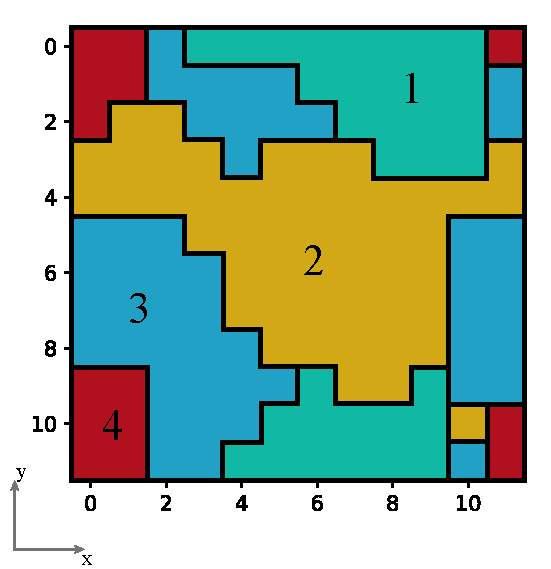
\includegraphics[scale=1]{figures/chapter2/Z2xZ2xZ2Z2domainWallsSlice.pdf}
	\caption{Planar snapshot along the $z$ axis of a Monte Carlo quench for the three copy model deep in the Higgs phase $J_1=J_2=J_3=0.8$ and $K=0$. This reveals the presence of the 4-state Potts model domains of Fig.\ref{threecopyexample} separated by the ``registry'' domain walls. Domain 1 - \fcolorbox{black}{z1}{\rule{0pt}{6pt}\rule{6pt}{0pt}} are $\uparrow \uparrow \uparrow \leftrightarrow \downarrow \downarrow \downarrow$, domain 2 - \fcolorbox{black}{z2}{\rule{0pt}{6pt}\rule{6pt}{0pt}} are $\downarrow \uparrow \uparrow \leftrightarrow \uparrow \downarrow \downarrow$, domain 3 - \fcolorbox{black}{z3}{\rule{0pt}{6pt}\rule{6pt}{0pt}} are $\downarrow \uparrow \downarrow \leftrightarrow \uparrow \downarrow \uparrow$, domain 4 - \fcolorbox{black}{z4}{\rule{0pt}{6pt}\rule{6pt}{0pt}} are $\uparrow \uparrow \downarrow \leftrightarrow \downarrow \downarrow \uparrow$. Every domain wall differs from the neighboring domain by a single flip.}
	\label{Z2xZ2xZ2Z2snapshot}
\end{figure*}

As for the two copy case one can now proceed by switching on  various $J_L^{ab}$ local couplings, ``gluing together''  the local matter copies with the expected results that we checked. Involving one coupling between two of the three sectors, the 4-state Pott symmetry is lifted by the explicit symmetry breaking to the effective two copy registry Ising symmetry. Similarly, coupling all copies with each other diminishes the registry spontaneous symmetry breaking such that confinement and Higgs become indistinguishable. In the same guise one can detune the matter couplings $J_a$, turning into a variation of the matters we discussed in the previous section. 

The two and three copy cases reveal the counting rules and by induction we can generalize this now to an arbitrary number copies. We just proceed as for the three copy case. Given $N_{\text{rep}}$ copies there are a total of $2^{N_{\text{rep}}}$ local configurations in unitary gauge. The next observation is that these configurations are pair wise identified with each other by the gauge transformation. The result is that the registry symmetry is now captured by a $p = 2^{N_{\text{rep}}} /2 $ state Potts model. 

\section{Replicating $O(2)$ matter.}
\label{replO2}

\begin{figure*}[!h]
	\centering	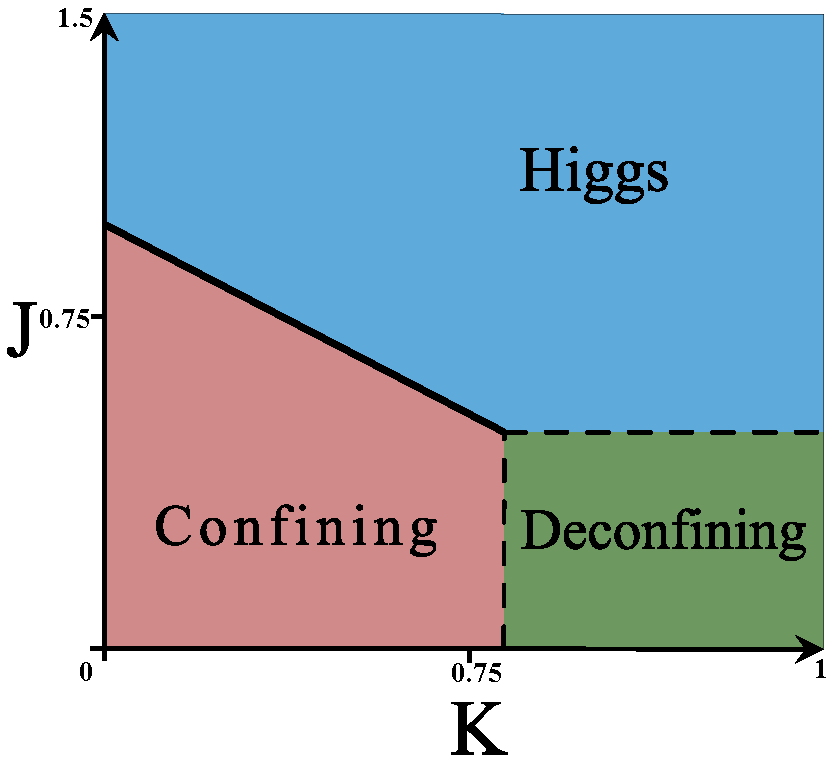
\includegraphics[width=0.425\textwidth]{figures/chapter2/O2xO2Z2phasedia.pdf}
	\raisebox{-.13in}{
		\includegraphics[width=0.45\textwidth]{figures/chapter2/O2xO2Z2}}
	\caption{The phase diagram of the $O(2) \cross O(2) / Z_2$ (left) and raw MC data for $c_V$(right) for $J_1 = J_2 = J$ and $J_L^{12} =0$. This is yet again remarkably similar as to the other phase diagrams. The difference is that the Higgs-confinement phase transition is now first order all the way to $K=0$ contrasting with its second order behavior for the single copy version, Fig.\ref{O2Z2phasediagram}. This due to the occurrence of a Ising type registry order parameter in the Higgs phase which is of the same kind as for the $Z_2$ matter cases, that disappears simultaneously with the nematic type order parameter upon entering the confining phase. The first order nature is confirmed by a Binder cumulant study (Fig.\ref{weakfirstorder}{\textbf{(c)}} in Appendix \ref{binder}).}
	\label{O2xO2Z2phasediagram}
\end{figure*}



The ``matter in the fundamental'' $Z_2$ matter case is special, and what to expect when the symmetry of the matter field is raised relative to the $Z_2$ gauge 
symmetry? For this purpose we focused in on the minimal extension: the replicated $O(2)$ matter fields gauged by $Z_2$. As we discussed in Section \ref{Z2Z2review}, for a single copy the Higgs phase is now characterized by the nematic-like order, distinguishing it from the confining phase through the presence of a second order phase transition.

In Fig.\ref{O2xO2Z2phasediagram}  we show the phase diagram of the two copy $O(2)\cross O(2)/Z_2$ case for the (usual) choice $J=J_1=J_2, J_L^{12} = 0$. This looks yet again very similar as to the other cases, the main difference being that now the transition between the Higgs and confining phase has turned into a {\em first order} transition for {\em all} $K$. Inspecting the ``strength'' of the first order transition exploiting the Binder criterium (see Appendix \ref{binder}) we find that close to the tricritical point the transition looks quite like the other cases: this is clearly driven by the ``Huse-Leibler'' amplitude fluctuations. Upon reducing $K$ the transition becomes an increasingly weak first order transition, but it continues to be first order all the way down to $K \rightarrow 0$.

As we will argue, this first order behavior is due to the fact that {\em two order parameters governed by two independent global symmetries vanish simultaneously}  at the Higgs to confinement transition. In fact, the replicating has the effect that the ``accidental'' second order nature of this transition for $O(2)/Z_2$ becomes similar to the generic first order transition of the $O(N)/Z_2$ system with $N \ge 3$ as argued by Ref. \cite{toner95}.

What are the two symmetries that are broken in the Higgs phase?  This is actually a bit more of a subtle affair than for the simple $Z_2$-replica's. As we will argue and confirm with the Monte Carlo, one type of symmetry is associated with the nematic type ``halved periodicity'' XY as for a single $O(2)/Z_2$, actually applying to both copies individually. But these are non-locally coupled together by the gauge fluctuations in a way that they submit to a perfect $Z_2$ registry symmetry, that is macroscopically the same symmetry as the registry $Z_2$ of the $Z_2\times Z_2/Z_2$ theory.        

This is yet again easy to deduce by zooming in on the maximal gauge fluctuations, the $K=0$ case. As discussed in Section \ref{replZ2}, this is of the universal form Eq.(\ref{Z2deGennes}). For the two copy $O(2) \times O(2)/Z_2$  case it follows immediately,
\begin{equation}
	\begin{split}
	&H_{O(2) \times O(2), K \rightarrow 0} =  -J' \sum_{\langle i, j \rangle} \left( \vec{\Phi}_{i1} \cdot  \vec{\Phi}_{j1} + \vec{\Phi}_{i2} \cdot  \vec{\Phi}_{j2} \right)^2 \\
		&\sim -J' \sum_{\langle i, j \rangle}  \left( ( \vec{\Phi}_{i1} \cdot  \vec{\Phi}_{j1})^2  + (\vec{\Phi}_{i2} \cdot  \vec{\Phi}_{j2})^2 +2 (  \vec{\Phi}_{i1} \cdot  \vec{\Phi}_{j1} ) \times ( \vec{\Phi}_{i2} \cdot  \vec{\Phi}_{j2}   ) \right) \mathperiod
	\end{split} 
	\label{O2O2effH}
\end{equation}
The first and second term just represent the director order parameter -- for $O(2)$ just the halved periodicity -- and upon ignoring the last term one is just dealing with two completely decoupled identical "$O(2)$ nematics".  This last term encapsulates the interactions between these two copies as induced by the fluctuating disclinations. It is obvious that also this term is governed by an invariance under $O(2)$ rotations of every copy separately -- there is surely no effective single site "anisotropy" at work reducing  it to the on site  $Z_2$ registry revealed by Eq. (\ref{twocopyZ2deGennes}) of the $Z_2 \times Z_2 / Z_2$ case.

However, the registry is now hidden in the "synchronization" imposed by the gauge fluctuations associated with the relative orientation of the two spin configurations on neighbouring sites.  Parameterize $\vec{\Phi} = | \Phi | e^{i \phi}$, such that $\phi_{j a} = \phi_{i a} + \nabla_{ij} \phi_a$ and the interaction term becomes,
\begin{equation}
	-J' \sum_{\langle i, j \rangle} (  \vec{\Phi}_{i1} \cdot  \vec{\Phi}_{j1} ) \times ( \vec{\Phi}_{i2} \cdot  \vec{\Phi}_{j2}   ) =   -J' | \Phi |^2 \sum_{\langle i, j \rangle} \cos ( \nabla_{ij} \phi_1 ) \cos(  \nabla_{ij} \phi_2) \mathperiod
	\label{O2O2dyn}
\end{equation}
This interaction term is governed by a global $Z_2$ symmetry! It originates in the synchrony of gauge invariant ``remnants'' of the two copies: the interaction term is minimal either for {\em both} copies being parallel on neighbouring sites  or {\em both} antiparallel where $\nabla_{ij} \phi_a=0$ or $\nabla_{ij} \phi_a=\pi$.  This signals the two fold degeneracy of the Ising order. In Fig.\ref{O2O2Z2order} we illustrate how to  construct the Ising domain walls associated with this registry order.  

\begin{figure*}[!h]
	\centering
	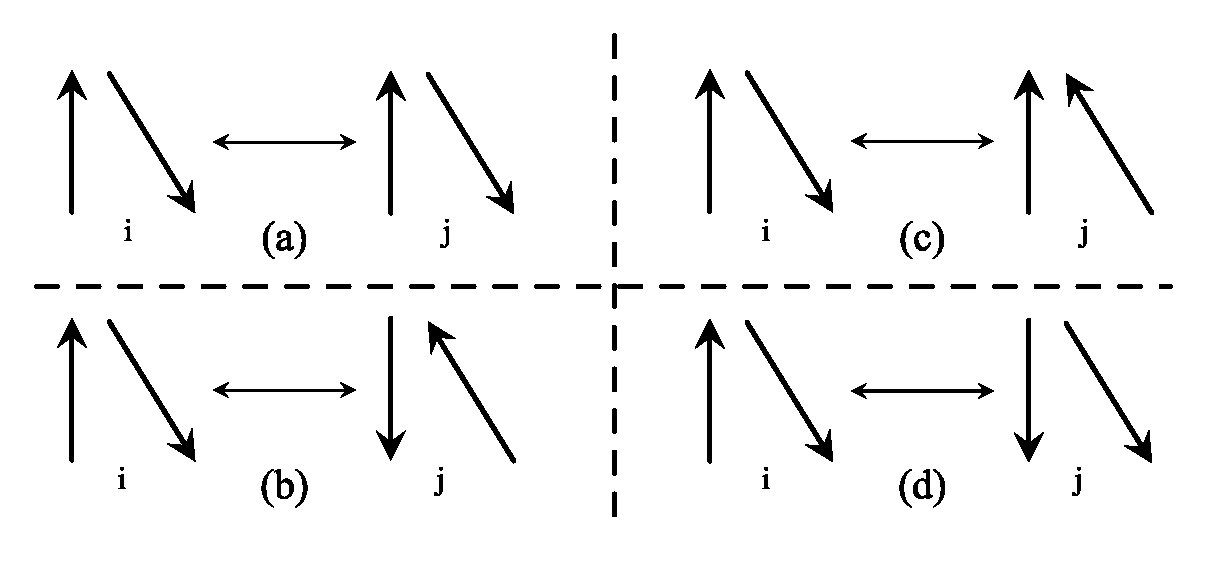
\includegraphics[scale=.5]{figures/chapter2/O2xO2Z2order.pdf}
	\caption{Illustration of the registry order of the  $O(2)\cross O(2) / Z_2$ theory: the construction of the registry Ising domain wall. We see that in contrast with the multiple $Z_2$ matter fields --- the \textit{local onsite} orientation of different matter fields is irrelevant for the registry. The two copies acquire independent orientations on the $O(2)$ (half) circle.   
		What matters is how two matter fields change {\em together} from site to site. The strong gauge field fluctuations ``glue'' together matter fields in a sense that they would have to simultaneously change together in the same direction, see Eqs.\eqref{O2O2effH},\eqref{O2O2dyn}.  In all cases \textbf{(a)}-\textbf{(d)} we depart from the same unitary gauge two spin reference configuration on site $i$. In \textbf{(a)} we just consider the ground state configuration on site $j$ in unitary gauge. By performing a gauge transforming on site $j$ we obtain  \textbf{(b)}, gauge equivalent  to \textbf{(a)}. But now consider  \textbf{(c)}, with an anti-parallel orientation of the second spin on site $j$, %turning into the
		gauge equivalent with \textbf{(d)}. 
		The case 	\textbf{(a)}, \textbf{(b)} corresponds with $\nabla_{ij} \phi_1 = \nabla_{ij} \phi_2=0$. We see that these configurations minimize the interaction energy Eq.\eqref{O2O2dyn}.  While \textbf{(c)}, \textbf{(d)} instead has $\nabla_{ij} \phi_1 =  0, \nabla_{ij} \phi_2=\pi$. Compared to \textbf{(a)}-\textbf{(b)} this would cost us $2J^{\prime}$ energy. The configuration \textbf{(a)}-\textbf{(b)} corresponds with a registry domain wall  between \textit{parallel} and \textit{anti-parallel} orientations of $O(2)$ matter directors at the neighboring sites.}
	\label{O2O2Z2order}
\end{figure*}




\begin{figure*}[!h]
	\centering
	\includegraphics[width=0.45\linewidth]{figures/chapter2/O2xO2Z2domainWallsSlice.pdf}
	\includegraphics[width=0.45\linewidth]{figures/chapter2/O2xO2Z2domainWallsNematicSlice.pdf}
	\caption{2D snapshot along $z$ axis of a system on $12\cross12\cross12$ lattice with periodic b.c for $O(2) \times O(2) / Z_2$  model. We a single frozen configuration of fields computed using a Monte Carlo quench deep in the Higgs phase: $J_1=J_2=5$ and $K=0$. \textbf{(Left)} Snapshot of $\cos(\nabla_{ij}\phi_1)$. This elucidates a simple registry order (parallel/anti-parallel), in the form of registry domains that are frozen in. The color coding denotes the cosine of the relative orientation of the spins on the neighboring sites: Domain 1 (parallel) - \fcolorbox{black}{z3}{\rule{0pt}{6pt}\rule{6pt}{0pt}} corresponds with $\uparrow \uparrow \leftrightarrow \downarrow \downarrow$, and domain 2 (anti-parallel) - \fcolorbox{black}{z4}{\rule{0pt}{6pt}\rule{6pt}{0pt}} accordingly  $\downarrow \uparrow \leftrightarrow \uparrow \downarrow$. \textbf{(Right)} Snapshot of $\exp(2i\phi_1)$ director order parameter showing homogeneous distributions, being annealed, with some local fluctuations due to the finite size and temperature effects.}
	\label{O2O2Z2snapshot}
\end{figure*}

This can be illustrated by a Monte-Carlo quench from ``high temperature'', departing from random configurations and partially annealing the system in the Higgs regime, similar to Fig.\ref{Z2xZ2xZ2Z2snapshot}. This is shown in Fig.\ref{O2O2Z2snapshot}. One infers that one form of order is of the nematic-type (XY like)  associated with the orientation of the director of one of the the copies that we find to be homogeneous in this snapshot -- this is annealed. However we can also track the {\em relative orientation of a single field between neighboring sites} $\nabla_{ij}\phi_\alpha$, for $\alpha=1$. Fig.\ref{O2O2Z2snapshot} (Left) shows that this is either parallel $\nabla_{ij}\phi_1=0$ or anti-parallel $\nabla_{ij}\phi_1=\pi$ as illustrated in Fig.\ref{O2O2Z2order} and explained after the text. As in Fig.\ref{Z2xZ2xZ2Z2snapshot} we observe domains of the two different parallel and anti-parallel registry separated by ``registry domain walls'' of the kind similar to the $Z_2$ matter.

Similar to the $Z_2\cross Z_2/Z_2$ case, this registry order is critically dependent on the $J_L^{12}$ being zero -- upon switching it on this acts as an explicit symmetry breaking of the registry turning the first order transition near $K=0$ into second order, exhibiting a phase diagram that is like the single  copy $O(2)/Z_2$ case (Fig.\ref{O2Z2phasediagram}). The effect of unbalancing the matter couplings ($J_1 \neq J_2$) has very similar effects as illustrated in Fig.\ref{Z2xZ2Z2Jl}, although now a second order transition is left behind when the registry order switches off.

In summary, the ``registry-sector'' of the $O(2)$ case behaves more or less identically as in the $Z_2$ case. The difference is that in the $O(2)$ case one also has to account simultaneously for the nematic type order characterizing this Higgs phase. This renders the phase transition first order all the way to $K=0$. 
The topological defects of this nematic-like state will start to populate the vacuum upon lowering $K,J$. These are the disclinations, in turn being a ``confined'' combination of the vortex-type matter defect, and the $Z_2$ gauge flux/vison, e.g. \cite{toner95,Senthil}. The matter-vortices of the two copies share a single gauge flux. Upon integrating out these ``topological fluctuations'', an interaction mediated by the $Z_2$ gauge fields develops which is responsible for the registry order.   Similar to the $Z_2$ case, the limit where one can easily deduce the effects of the visons ``gluing'' the copies into registry, this is most easily deduced in the $K=0$ limit which is entirely controlled by the matter interaction $J$.    

\section{Discussion and conclusions}
\label{discussion}

Gauge field theory is of course well known to have its own rules. In this paper we have focused in on the simplest of all gauge symmetries, the $Z_2$ variety, as the simplest theory revealing the characteristic phase structure characterized by confinement, deconfinement and the Higgs phase. By introducing the matter replicas we discovered a new set of phenomena. In this pursuit we have heavily leaned on the unbiased Monte-Carlo simulations. Puzzled by the outcomes we discovered the new phenomenon of ``registry order parameter''. As we discussed in Sections \ref{replZ2} and \ref{replmanyZ2}, it is very easy to identify the origin in the $Z_2$ matter versions, although it is a bit less obvious and arguably more entertaining  for the $O(2)$ version in Section \ref{replO2}. It took us by surprise, given that the origin of the induced ``gauge interaction'' that is responsible for the registry symmetry breaking  is of a kind that is rather unfamiliar.  

The mechanism is revealed by considering the extreme strongly coupled limit of the gauge fields, $K=0$. In terms of the degrees of freedom of the gauge theory, the mechanism is unusual, highlighted by the $O(2)$ case. The physical degrees of freedom associated with the disordering of the Higgs phase are the nematic-type disclinations that are in turn confined combinations of matter vortices and the fluxes of the gauge field (the visons). Although both matter fields carry their own vortices, these ``share'' a single vison. In the $K=0$ limit the latter come for free and upon integrating these out one finds that the de-Gennes type effective order parameter theory is endowed with the registry ``Ising'' Hamiltonian, Eq . (\ref{twocopyZ2deGennes}), and Eq.(\ref{O2O2dyn}) respectively. Interestingly, the discrete nature of the gauge theory has eventually the effect to generate the Ising type registry global symmetry breaking. 

We have only inspected the most elementary forms of such gauge theoretical systems. 
These are just a point in the vast landscape of all gauge theories, up to the non-Abelian Yang-Mills theory behind e.g. the Standard Model. It would be quite interesting to find out what happens with this ``registry order'' upon systematically raising the symmetries involved. What happens in the ``replicated''  $Z_2$ gauge theory involving the non-Abelian $O(N)$ matter fields with $N \ge 3$? What happens raising the $Z_2$ gauge symmetry to the non-Abelian 3D point group symmetries as in Ref. \cite{nonabnematic}? Even more fundamental, what is the fate of registry dealing with {\em continuous} gauge symmetry, starting with the Abelian $U(1)$ of compact electrodynamics \cite{PolyakovQED}? 

Finally, another aspect also caught us by surprise in the Monte Carlo outcomes for the various phase diagrams. The Huse-Leibler mechanism for the first order transition between the "Higgs'' and "confinement-like phase'' emanating from the tricritical point appears to be surprisingly universal. Eventually this is a quantitative affair. The mechanism as understood for the $Z_2/Z_2$ case does in this regard rely on the specifics of this particular theory: the ``vesicles'' versus ``platelet'' affair. This surely works differently involving continuous symmetry -- the $O(2)$ cases. But surprisingly the ``first order strand'' is even quantitatively barely affected by these fundamental differences. The reason for this is presently unclear to us and it may be of interest to have a closer look at the origin of this ``quasi-universality''.

\section*{Acknowledgments}
We thank T. Senthil and K. Liu for discussions. 
This research was supported in part by the Dutch Research Council (NWO) project 680-91-116 ({\em Planckian Dissipation and Quantum Thermalisation: From Black Hole Answers to Strange Metal Questions.}), and by the Dutch Research Council/Ministry of Education. The numerical computations were carried out on the Dutch national Cartesius and Snellius national supercomputing facilities with the support of the SURF Cooperative as well as on the ALICE-cluster of Leiden University. We are grateful for their help.


\section{Appendix}
\subsection{Monte Carlo Simulations}
\label{app:mc-details}
The Monte Carlo simulations were performed on a $d \times d \times d$ grid with periodic boundary conditions. Grid size in all simulations was $d=12$ in order to avoid finite size effects and still get reasonable computational times. We used most of the time a number of  measurement sweeps $N=6000000$; thermalization sets in typically after 1/3 of the sweeps. Near the critical points we checked this by tracking the evolution of the various quantities  as function of the number of steps, taking as many steps as needed for the quantity to saturate. For the updating rules we used the  Metropolis-Hastings algorithm with the acceptance ratio $A(n, n^\prime) = \min(1, e^{-\Delta E_{n,n^\prime}})$ where $\Delta E_{n,n^\prime}$ is the energy difference between states $n$ and $n^\prime$ that differ in a single matter field or gauge field flip. Phase diagrams were obtained by vertically scanning along different values of $J$'s, using annealing order to improve convergence accuracy. The whole phase diagram was run on a remote cluster where each process was  associated with a single value of $K$ scanning along the $J$ axis. We noted that the longest sweeps were required to equilibrate when deep in the deconfining regime. Flipping single ``bond spins'' using the Metropolis-Hastings algorithm leads to highly energetic configurations and accordingly to long thermalization times. But this did not pose any difficulty since the physics in this regime is simple.

\subsection{Determining order of phase transition}
\label{binder}
We used several quantities in order to determine the order of a phase transition. For the $O(2)$ matter fields we tracked  the  local nematic magnetization $m=\langle |e^{2i\theta_i}|\rangle$ and local registry order parameter $R=\langle \theta^1_i \cdot \theta^2_i \rangle$. For $Z_2$ matter fields we only encountered the local registry order parameter. Note that formally the $O(2)\cross O(2)/Z_2$ registry order parameter is non-local in that it is the nearest neighbor difference. In practice this implies also a local order parameter, which is easy to understand after performing a ``block-spin'' averaging RG-step. We also measured  the specific heat computed as $C_V = \frac{1}{d^3}(\langle E^2 \rangle -\langle E \rangle)$. In order to see the exact point of phase transition we employed the Binder ratio defined as: 
\begin{equation}
	U = \frac{1}{2} \left[3 - \frac{\langle m^4\rangle}{\langle m^2 \rangle^2}\right] \mathperiod
\end{equation}
In the $\lim_{T \to 0} U = 1$ while for $\lim_{T \to \infty} U = 0$. Since this ratio is dimensionless, plotting curves of different sizes clusters their intersection point which represents the exact value of the phase transition. In our case shape of the Binder curve is more important than the exact intersection point. A smooth transition from 0 to 1 in a sigmoid fashion indicates a second order transition while a sharp dip that diverges with system size indicates a first order behavior. Especially the transition associated with the small $K$ regime of the $O(2) \cross O(2) / Z_2$ is quite weakly first order, and this is manifested by a Binder ratio dip that does not diverge with the system size, see e.g. and Fig.\ref{weakfirstorder}(\textbf(c)). When going to larger system sizes, dip in the Binder curve become very narrow. In that case, refining values of $J$ in that regions helps capture it, otherwise the peak is easily missed.  

\begin{figure}[!h]
	\captionsetup[subfigure]{labelformat=empty}
	\centering
	\begin{subfigure}{0.45\textwidth}
		\centering
		\includegraphics[width=\columnwidth]{figures/chapter2/BinderSecondExample.pdf}
		\caption{\textbf{(a)}}
	\end{subfigure}%
	\begin{subfigure}{0.45\textwidth}
		\centering
		\includegraphics[width=\columnwidth]{figures/chapter2/BinderFirstExample.pdf}
		\caption{\textbf{(b)}}
	\end{subfigure}
	\par\bigskip
	\begin{subfigure}{0.45\textwidth}
		\centering
		\includegraphics[width=\columnwidth]{figures/chapter2/BinderK0O2xO2Z2.pdf}
		\caption{\textbf{(c)}}
	\end{subfigure}%
	\begin{subfigure}{0.45\textwidth}
		\centering
		\includegraphics[width=\columnwidth]{figures/chapter2/BinderK0Z2xZ2xZ2Z2.pdf}
		\caption{\textbf{(d)}}
	\end{subfigure}
	\caption{Examples of the Binder ratio as function of system size: (\textbf{a}):  A typical example of a second order transition from confining to Higgs for $O(2)/Z_2$ at $K=0$, (\textbf{b}): An example of a first order transition for $O(2)/Z_2$ at value of $K$ in the range of first order - "Huse-Leibler" line emanating from the tricritical point (\textbf{c}):  An example of the Binder ratio for a weak first order transition, showing its behavior for $O(2) \cross O(2) / Z_2$ for  $K=0$ as function of $J$. (\textbf{d}) An example of the Binder ratio for $Z_2 \cross Z_2 \cross Z_2 / Z_2$ along $K=0$ with a clear indication of a second order phase transition.}
	\label{weakfirstorder}	
\end{figure}

Besides the Binder ratio we also inspected histograms of values occurred during the run of a simulation for an average spatial order parameter and the local energy in order to observe the detailed behavior around the critical point where more than one peak signals the phase separation associated with first order transitions. Histogram are created by counting the occurrences of observed value in specific predetermined bins. Even with fluctuations happening during the run of a simulation, these graphs reveal where are the points of most concentrations around which quantity varies. In most simulations size of the single bin was $10^{-5}$ in single unit of observed quantity, which helps in a resolution of very closely placed peaks. As an example of usefulness of distribution histograms in determining the order of a phase transition we present ``registry'' and energy distributions for $Z_2 \cross Z_2 / Z_2$ model for single value of $K=0.55$ in the regime of ``Huse-Leibler'' first order line emanating from the tricritical point, Fig.\ref{distributions}.

\begin{figure*}[!h]
	\centering
	\includegraphics[scale=.7]{figures/chapter2/Z2xZ2Z2K57.pdf}
	\caption{Example of average order parameter ($\langle \theta^1_i \cdot \theta^2_i \rangle$) and energy ($E$) distributions values during a single run of a simulation, on the ``Huse-Leibler'' first order line $J=0.29, K=0.55$ , for $Z_2 \cross Z_2 / Z_2$ model with the usual $J=J_1=J_2$ and $J_L^{12}=0$. We see the appearance of two peaks in these distributions indicating the coexistence of two phases.}
	\label{distributions}	
\end{figure*}


All the phase diagrams presented in this paper are graphs of specific heat. But for determining the precise nature of the phase order that is not enough. As it can be seen from raw data graphs absolute values of specific heat can be an indicator of the order, but can't be completely trusted, because these values depend on the model and are not universal. We only used specific heat as an indicator of where the transition might be Fig.\ref{cvExample}, but analysis using Binder and histograms were done to determine the order of the transition.
\begin{figure*}[!h]
	\centering
	\includegraphics[scale=.7]{figures/chapter2/cvExample.pdf}
	\caption{Example of the specific heat $c_V$ for $O(2) \cross O(2) / Z_2$ (blue-dots) and $O(2)/Z_2$ (red-cross) along the $K=0$ slice (Higgs to confining transition). These two models have a different order of a phase transition which might be seen from the amplitude of a $c_V$ divergence. Usually sharper and bigger divergences indicate the first order has occurred. However, one has to be careful due to finite size effects, and for this reason we also study the Binder cumulants. Better use for this graphs is in roughly locating where the transition happens. This information can be used to run the simulation on a more finely spaced grid around the transition in order to get better convergence and more precise point of transition using finite size methods.}
	\label{cvExample}	
\end{figure*}
		%\chapter{A BCS-Josephson Wormhole in coupled superconducting Yukawa-SYK metals}
\label{chap:JosephsonWormhole}

\section*{Attribution}
The work in this chapter has been done jointly with Stephan Plugge and Koenraad Schalm, and is a manuscript under preparation.

% \begin{abstract}
\section*{Abstract}
\noindent
We show that two Yukawa-SYK models with a weak tunneling contact can have an exotic superconducting hybrid thermofield-double-like state holographically dual to a traversable wormhole connecting two black holes with charged scalar hair. 
% For strong tunneling this state crosses over to a conventional Josephson contact. 
The hybrid thermo-field-double/wormhole state is distinguishable by anomalous scaling of revival oscillations in the fermionic Green's function, while the BCS-like superconducting condensate is responseless. 
% This is a correlated with emergence of the superconducting state of Yukawa-SYK models emerges out of a quantum critical strange metallic normal state by the BCS-like opening of a gap \as{I'm not sure what the previous sentence is supposed to convey}. 
The existence of this TFD/wormhole state surprisingly shows that the some quantum critical effects can survive the phase transition to superconductivity. It also suggests a more strange metallic TFD/Josephson wormhole can exist correlated with superconductivity at strong coupling, where Cooper pairs persist above the critical temperature.
% \comment{DO YOU HAVE A FIGURE THAT SHOWS THE OPENING OF THE BCS GAP?}\as{no - I haven't had time to do the real time numerics including superconductivity}
% \comment{OK, Let's leave it to the reference to \cite{esterlis2021large} as we do now. Comment these comments out, when you agree.}
% \end{abstract}

%\keywords{Suggested keywords}%Use showkeys class option if keyword
                              %display desired
% \maketitle
%\tableofcontents

\section{Introduction}
\label{sec:introduction}

\noindent
The realization that the quantum critical strongly correlated groundstate of the Sachdev-Ye-Kitaev model 
%of disorder averaged interacting fermions 
is in the same universality class as the groundstate of holographic models of charged anti-de-Sitter black holes has opened up a wide avenue to study exotic gravitational questions with quantum-mechanical Hamiltonians. One such question is the existence of traversable wormholes. Maldacena and Qi \cite{maldacena2018eternal}, based on an earlier work of Gao, Jafferis and Wall \cite{gaoTraversableWormholesDouble2017} and more recently others \cite{maldacenaDivingTraversableWormholes2017,maldacenaTraversableWormholesFour2020,bakBulkViewTeleportation2018,gaoRegenesisQuantumTraversable2019,fuTraversableAsymptoticallyFlat2019,bakExperimentalProbesTraversable2019,qiCoupledSYKModel2020a,caceres2021sparse,haenel2021traversable,berenguer2024floquet},
%\comment{CHECK ALL/MORE}\as{done}, 
showed that (marginally) relevant tunneling interactions between two such SYK Hamiltonians could induce a phase transition to a finite temperature ``wormhole'' state as the temperature is lowered. The quantum mechanical understanding of this transition is as follows. At high temperatures, where tunneling is minimal, the state of the coupled system is arbitrarily close to two independent decoupled thermal ensembles at high temperature --- holographically dual to two black holes
\begin{align}
\label{eq:2BH-densitymatrix}
    \rho_{\text{2BH}} = \frac{1}{Z_{\beta}^2}\sum_{n_1,n_2} e^{-\beta (H_1+H_2)} |n_1,n_2\rangle\langle n_1,n_2|~.
\end{align}
The density matrix can also be written as a state in a doubled system
\begin{align}
\label{eq:2BH-state}
|\text{2BH}\rangle_{\beta} = \frac{1}{Z_{\beta}^2}\sum_{n_1,n_2} e^{-\beta (E_{n_1}+E_{n_2})} |n_1,\bar{n}_2\rangle~,
\end{align}
where $|\bar{n}\rangle = |\Theta n\rangle$ with $\Theta$ an anti-unitary symmetry of the SYK model (usually CPT).
As one lowers the temperature and the tunneling becomes stronger the thermodynamically preferred state is a different one. This is the state close to the maximally entangled so-called Thermo-Field-Double state --- holographically dual to a wormhole connecting the two black holes
\begin{align}
\label{eq:WH-state}
    |\text{WH}\rangle_{\beta} =|\text{TFD}\rangle_{\beta} = \frac{1}{\sqrt{Z_{\beta}}}\sum_n e^{-\frac{\beta}{2}E_{n}} |n,\bar{n}\rangle
\end{align}
Here $Z_{\beta}=\sum e^{-\beta E_n}$ is the partition function of a single SYK model.

Macroscopically it is a first order transition driven by the relevancy of the tunneling interaction, but the telltale sign of the wormhole is more subtle than a macroscopic order parameter. When the high temperature state is %still 
in the strongly correlated regime such that it is the finite temperature extension of the quantum critical SYK groundstate dual to a black hole, rather than a thermal gas of free quasiparticles, the low temperature ``wormhole'' state can remember this critical origin in that its spectrum can be better explained as a perturbation of its quantum critical spectrum rather than a perturbation around a free system. Specifically, the near-AdS$_2$ symmetry group (time-reparametrizations modulo $PSL(2)$) that defines the quantum critical state of a single SYK system, continues to determine the spectrum of the coupled system even when the groundstate changes to the TFD/WH state \cite{maldacena2018eternal}. This deformed N-AdS$_2$ spectrum has a uniquely characteristic fixed spacing between levels similar to that of a harmonic oscillator: $E_n = E_{\text{gap}}(1+ \frac{1}{\Delta}n), n \in \mathbb{N}$, with the groundstate energy $E_{\text{gap}}\sim \lambda^{\frac{1}{2-2\Delta}}$ proportional to a non-perturbative non-analytic fractional power of the tunneling strength $\lambda$ in terms of the IR critical scaling dimension $\Delta$ of a fermionic excitation. This fixed integer spacing in units of $c$ is observable in characteristic revivals in a linear response probe, as convincingly shown in subsequent numerical simulations \cite{maldacenaSYKWormholeFormation2020a,pluggeRevivalDynamicsTraversable2020a,sahooTraversableWormholeHawkingPage2020,qiCoupledSYKModel2020a}. %\comment{CHECK}\as{done}. 
From the dual holographic gravitational perspective this revival is a perturbation that has fallen into a black hole, traveled through the wormhole and back. One should be careful: Revival-signatures in linear response can have many origins and not all revivals are dual to a signal traversing a wormhole. The key aspect is the non-analytic dependence of the gap $E_{\text{gap}}$ and the spacing $\Delta E =E_{\text{gap}}/\Delta$ on the relevant tunneling strength $\lambda$. Even within these SYK-models, if this relevant coupling becomes strong, the system still shows revivals. But as the system has now crossed over to a free-fermion state, the gap and the level spacing underlying the revivals are now an integer analytic power of tunneling strength. It is just a reflection of the regularity of the underlying standard free particle harmonic oscillator spectrum. 
Fig.\ref{fig:Schematic Phase diagram}A summarizes this phase diagram of the 2BH/WH transition in quantum critical SYK models.




However theoretically appealing, in actual physical systems quantum critical states are rare. Moreover, experimentally they are fragile and extremely susceptible to decay to a conventional ordered state, usually a BCS superconductor. It is conjectured that in 2D systems this is in fact always the case \cite{metlitskiAreNonFermiliquidsStable2015,abanov2020interplay,chubukov2020interplay}.
The SYK-like quantum critical systems are essentially 0D quantum dots, but 2D extensions can preserve many of its features including the N-AdS$_2$ like structure of its groundstate \cite{patel2023universal}. Some of the fragility of this quantum critical grounstate is suppressed by a large $N$-limit, but some is also by construction. In particular the simplest SYK models do not preserve time-reversal symmetry and singlet Cooper pairs are not stable enough to form a long range coherent state. More realistic models must preserve (some) time reversal symmetry to allow pairing. One such model is the Yukawa-SYK model constructed in \cite{esterlis2019cooper}. This is a quantum critical superconductor with a tunable pairing strength and $T_c$ whose condensate is not controlled by the density of states at the Fermi surface \cite{sheBCSSuperconductivityQuantum2010,esterlis2019cooper}. 
%\comment{CHECK FIRST REFERENCE.}\as{done} 
In particular, the charge neutral critical state with no Fermi surface is already unstable towards superconductivity. It is able to do so as the density of states is large even at charge neutrality, which allows a macroscopic condensate to form.
%\comment{CHECK}
For a large part of the phase diagram this superconductivity indeed prevents the emergence of quantum criticality, but this view has been challenged recently in Ref.~\cite{zhang2023density}.


The question we address in this article is whether the exotic revival physics dual to a wormhole state persists in tunneling contacts between such more realistic SYK models as Yukawa-SYK that do exhibit superconductivity. Naively one would think not, in accordance with the wisdom that superconductivity prevents quantum criticality. The onset of superconductivity gaps the low-energy spectrum and this ought to destroy to characteristic fixed level spacing responsible for the wormhole revival physics. The loophole is that in these models superconductivity is tunable and a window may exist that nevertheless allows for a sufficiently regular spectrum that a wormhole like state survives. The holographic gravitational dual of such a state would be a wormhole with a scalar condensate also known as scalar hair. An argument in favor that such state could result from this construction is the fact that the thermofield-double state is a formal purification of the straightforward thermal mixed state of a single YSYK model. It must therefore exist, and perhaps the better posed question is whether this protocol contructs the TFD-state as the groundstate of the coupled YSYK system.      

In this article we report that this indeed turns out to be the case and the loophole is realized --- in a particular way. There exists indeed a strongly entangled tunneling contact state between two superconducting YSYK systems that nevertheless has a low-energy spectrum controlled by the N-AdS$_2$ of the critical state. Pictorially this is represented in Fig. \ref{fig:Schematic Phase diagram}B.
The particularity of this state is that the regime where this state is found is one where superconducivity manifests itself in the fermionic spectrum by the BCS-like opening of gap. Qualitatively, this means that Cooper pairs condensate immediately upon binding and there are no uncondensed bound-fermion states in the spectrum. 
%In effect the TFD/wormhole state is not given by Eq.~\ref{eq:WH-state}, but by a state close to \comment{BETTER NAME}
%\begin{align}
%    |\text{partial}-WH\rangle_{\beta} = |\text{partial}-TFD\rangle_{\beta} = \frac{1}{Z_{\beta}} \sum_n_F e^{-\frac{\beta}{2}}|n_F,\bar{n}_F\rangle\otimes|0,0\rangle
%\end{align}
The ``wormhole'' state is therefore the honest TFD of the fermionic excitations on top of the BCS-like groundstate. This is in contrast to a more BEC-like superconductivity where bound states form first, exist as independent asymptotic excitations in the spectrum, and only condense at a lower temperature. In the fermionic spectral function this manifests itself as a depletion of the gap/growth of a peak at finite energy, as is observed in real high $T_c$ strange metals for instance \cite{kondoPointNodesPersisting2015,reberPairingPairbreakingTheir2015a,liCoherentOrganizationElectronic2018,bastiaansDirectEvidenceCooper2021,trompPuddleFormationPersistent2023}. The TFD/``wormhole'' state of such a system would have the same formal form as Eq.~\eqref{eq:WH-state}, but now the energy states would contain both fermionic and bosonic excitations. In principle the YSYK model we study has a regime where such BEC-like superconductivity occurs \cite{esterlis2019cooper}. However, generically this originates from an impurity-like normal state above $T_c$ and not from the quantum critical state holographically dual to black holes. We have therefore not studied this here.

Tunneling contacts between superconducting systems --- a Josephson junction --- are of course an enormously well studied and useful arena of physics. As the Josephson current is the tunneling of Cooper pairs, an immediate question is whether the %AC 
Josephson current can also show revivals characteristic of a ``wormhole''. 
Even if quantum in origin, the dominant Josephson effects are macroscopic thermodynamic manifestions: they are captured by the Landau-Ginzburg free energy. The universality of the latter precludes any significant change in observational responses due to an underlying TFD/wormhole state. We confirm this by a computation of the DC Josephson current in the TFD/wormhole state. Similar to non-superconducting SYK models, the manifestation of the wormhole is more subtle. A more fine grained analysis of Josephson physics may reveal other effects in addition to the single fermion revivals. We leave this for further study. 
%\comment{[DROP? BETTER NAME?]}
Nevertheless, as the superconductor-superconductor wormhole is supported by a tunneling interaction, to christen it the BCS-Josephson wormhole seems apt.



Section \ref{sec:model} describes the YSYK model, the tunneling interaction coupling two YSYK models and the effective Schwinger-Dyson equations controlling the large $N$-limit of the model after disorder averaging over random four-fermion interactions. Section \ref{sec:metallic-state} describes the TFD/wormhole state when superconductivity is artifially surpressed to connect with earlier coupled SYK wormhole results and set the stage for Section \ref{sec:sc-state} where we exhibit the existence of the BCS-Josephson wormhole, i.e. a thermodynamic phase transition to a superconducting TFD-state. From the free energy of the total system we compute the DC Josephson current to show that it is not affected by the underlying state change as could have been surmised by the fact that the TFD-state is thermodynamically in the same phase as the ordinary BCS state. We conclude with a brief outlook in the conclusion Section \ref{sec:conclusion}.


%To answer this requires a more detailed analysis than we present in this paper. We can, however,


\begin{figure}[t]
    \centering
    \includegraphics[width=0.9\linewidth]{figures/chapter3/2YSYK-PhaseDiagram-v3.pdf}
    \caption{
        Schematic phase diagram of two coupled Yukawa-SYK systems without (left) and with superconductivity (right). When superconductivity is suppressed, there is a first order phase transition at fixed $\lambda < \lambda_{\text{SYK}}$ for $T\sim \lambda$. There the system transitions from a intermediate temperature $T\lesssim T_{\text{SYK}}$ state of essentially two decoupled thermal strongly correlated SYK systems holographically dual to two black holes (2BH), to a low temperature thermofield double state with specific cross-correlations holographically dual to wormhole (WH).  At very high temperatures $T \gg T_{\text{SYK}}$ or very high tunneling coupling $\lambda\gg\lambda_{\text{SYK}}$ the coupled system is in a free fermion phases that are smoothly connected to each other. When superconductivity is included. The above is valid for an intermediate value of the averaged Yukawa-YK-coupling in terms of the bare boson mass $g_{\text{SYK}}/\omega^{3/2}\sim 0.5$, the two-black-hole phase first becomes a two essentially independent superconductor phase, holographically dual to two hairy black holes (2BH-SC). This state crosses over around the value of the putative 2BH/WH phase-transition to a excitation spectrum on top of the superconducting groundstate that is characteristic of the thermo-field-double/wormhole state.  %On lowering the temperature, we find first powerlaw correlations developing in the diagonal green's function. We call this non-fermi liquid state (NFL) which is dual to a two sided black hole geometry. At the lowest temperatures however, i.e. when $T \ll \lambda $, the system undergoes a first order transition to the wormhole state. The two phases are demarcated by a line $T \sim \lambda$. 
        %\comment{Include $T_{\text{SYK}}\sim g^{2/3}$ DONE; ALSO EDITED}
        }
    \label{fig:Schematic Phase diagram}
\end{figure}
%\comment{
%\begin{itemize}
%    \item {\bf Characteristics}
%    \item Josephson current
%    \comment{(four point function?)/Numerics}
%    \item 
%\end{itemize}
%}




%##################

\section{Two Yukawa-SYK models with a tunneling contact with shared disorder.}
\label{sec:model}

\noindent
The Yukawa-SYK model describes a quantum dots with $N$ flavors of spin-$\frac{1}{2}$ fermions and $M$ flavors of bosons with Hamiltonian \cite{esterlis2019cooper}
\begin{align}
       H_{\text{Y-SYK}} = -\mu\sum_{i=1}^N\sum_{\sigma=\uparrow,\downarrow} c^\dagger_{i,\sigma} c^{\phantom{\dagger}}_{i, \sigma} + \sum_{k=1}^M \frac{1}{2}\left(\pi_k^2 + \omega_0^2\phi_k^2\right) + \frac{\sqrt{2}}{N}\sum_{i,j,k}\sum_{\sigma}g_{ijk} c^\dagger_{i,\sigma} c^{\phantom{\dagger}}_{j,\sigma} \phi^{\phantom{\dagger}}_k~.
    \label{eq:HYSYK}
\end{align}
In a single instance of the model the complex couplings $g_{ijk}=g^{'}_{ijk}+ig^{''}_{ij,k}$ are randomly drawn from an ensemble with zero mean and variance
\begin{align}
    \langle g'_{ijk}g'_{lmn}\rangle &= (1-\frac{\alpha}{2})g^2\delta_{kn}(\delta_{il}\delta_{jm}+\delta_{im}\delta_{jl})~,\nonumber\\
    \langle g'_{ijk}g'_{lmn}\rangle &= \frac{\alpha}{2}g^2\delta_{kn}(\delta_{il}\delta_{jm}-\delta_{im}\delta_{jl})~,\nonumber\\
    \langle g'_{ijk}g''_{lmn}\rangle &=0~.
\end{align}
For $\alpha=1$ the hermitian matrix $g_{ijk}=(g_k)_{ij}$ is in the Gaussian Unitary ensemble; for $\alpha=0$ the matrix is real and in the Gaussian orthogonal ensemble. The model is solvable after averaging over the ensemble and taking the double limit $N\rightarrow \infty$, $M\rightarrow\infty$ with $\kappa=M/N$ fixed.
For $\alpha=1$ the system has a quantum critical SYK groundstate for any value of the chemical potential $\mu$ and boson mass $\omega_0$ with scaling dimensions $\Delta_f$ and $\Delta_b$ for the fermions and bosons respectively that are fixed by 
%Upon starting from the high temperature phase FF1 and lowering temperature below the scale $T_{SYK}$, we see the onset of the NFL state and its emergent conformal symmetry. At low frequencies, the diagonal Green's functions scale with a power law 
% \begin{align}
%     G(\omega) &\sim \abs{\omega}^{2\Delta_f-1}\sgn(\omega) \\
%     D(\omega) &\sim \abs{\omega}^{2\Delta_b-1} \,.
%     \label{eq:scalingsolns}
% \end{align}
% In these equations, $\Delta_f$ and $\Delta_b$ are the scaling dimensions of the fermions and bosons respectively, and can be calculated in the conformal limit of the Schwinger-Dyson equations. They need to satisfy
\begin{align}
\label{eq:YSYK-scaling-dims}
    2\Delta_f + \Delta_b &= 1 \, ,\non
    \kappa\frac{\Gamma(1-\Delta_f)\Gamma(1-(\Delta_f+\Delta_b))}{\Gamma(\frac{1}{2}+\Delta_f)\Gamma(\frac{1}{2}+\Delta_f+\Delta_b)} &= -2 \frac{\Gamma(\frac{1}{2}-\Delta_b)\Gamma(\frac{1}{2}-2\Delta_f)}{\Gamma(\Delta_b)\Gamma(2\Delta_f)} .
\end{align}
(see Appendix \ref{app:effectiveaction}). For $\alpha < 1$ the theory has a time-reversal preserving sector and allows for pairing and a stable superconducting phase. In particular, at $\alpha=0$ for a small range of $g \sim \omega_0^{3/2}$ the phase diagram (Fig.~\ref{fig:YSYK-phase-diagram}) has a small window where the onset of superconductivity occurs from the finite temperature extension of the quantum critical Yukawa-SYK N-AdS$_2$ state holographically dual to a black hole~\cite{esterlis2019cooper,wang2020solvable,classen2021superconductivity,inkof2022quantum}. We shall choose the model with $\alpha=0$ at charge neutrality $\mu=0$ with that value of $g/\omega_0^{3/2}=0.5$ and hold these fixed throughout this study; we shall also choose $\kappa=1$ throughout.
%\comment{CHECK}\as{correct}
What shall be important later in Section \ref{sec:sc-state}, is that for this value the onset of superconductivity manifests itself in the fermionic spectral function by the opening of a gap (Fig.~6 in \cite{esterlis2019cooper}), i.e. bound fermion states immediately condense and the spectrum of excitations does not contain bound-fermion states.
%\comment{CHECK}\as{correct}.

\begin{figure}[t!]
    \centering
    \includegraphics[width=0.5\linewidth]{figures/chapter3/YSYK-PhaseDiagram-v3.pdf}
    \caption{The phase diagram of a single Yukawa-SYK model with couplings drawn from the GOE from \cite{esterlis2019cooper}. FF is a free-fermion phase; BH is the finite temperature version of the quantum critical N-AdS$_2$ SYK groundstate dual to a black hole. SC is the superconducting state which has a crossover from BCS-like SC to BEC-like SC as $g/\omega_0^{3/2}$ increases. At high temperatures for large $g$ the model is controlled by an impurity fixed point. 
    The dashed line denotes the value of the disorder-averaged coupling $g/\omega_0^{3/2}=0.5$ we use in this in article such that the normal phase right above the superconducting transition is the quantum critical/BH phase.}
    \label{fig:YSYK-phase-diagram}
\end{figure}

The two coupled system configuration that allows for entangled TFD phase at low temperatures is constructed by coupling two identical Yukawa-SYK models, i.e. with the same random coupling constants {\em before disorder averaging}, together with a simple tunneling interaction.
% \begin{align}
%     H=H_{\text{YSYK}}^{(1)}[g_{ijk}] + H_{\text{YSYK}}^{(2)}[g_{ijk}] + \sum_{i,\sigma} \lambda c^{\dagger(1)}_{i\sigma}c^{(2)}_{i\sigma} +\lambda^\dagger c^{\dagger(2)}_{i\sigma}c^{(1)}_{L,i\sigma}~.
% \end{align}
%$
% are disorder-averaged 
% on each of them respectively, and described separately by the Yukawa SYK Hamiltonian, with exactly the same realization of disorder on each side. We are interested in this model in the of large fermion and boson flavors $M\rightarrow\infty$, $N\rightarrow\infty$, such that the ratio $\kappa = \nicefrac{M}{N}$ is constant.
%The two individual dots are then coupled by a fermion interaction across the two dots, of strength $\lambda$. 
The joined model is then described by the following action
% \begin{widetext}    
\begin{align}
    S &= S^{(1)}[g_{ijk}] + S^{(2)}[g_{ijk}] + S_c \, , \nonumber \\
    S^{(a)}[g_{ijk}]&= \int \!\dd\tau \sum_{i,\sigma} {c^\dagger}^{(a)}_{i\sigma}(\tau) \left(\partial_\tau - \mu\right)c^{(a)}_{i\sigma}(\tau) + \sum_k \phi^{(a)}_k(\tau)\frac{1}{2}\left(-\partial_\tau^2 + \omega_0^2\right) \phi^{(a)}_k(\tau) \nonumber\\
     &~~~~~~+ \frac{\sqrt{2}}{N}\int\!\dd\tau \sum_{ijk,\sigma} g_{ijk}{c^\dagger}^{(a)}_{i\sigma}(\tau)c^{(a)}_{j\sigma}(\tau)\phi^{(a)}_k(\tau) \, ,\nonumber\\
    S_c &= \int \!\dd\tau \sum_{i,\sigma}\lambda {c^\dagger}^{(1)}_{i\sigma}(\tau)c^{(2)}_{i\sigma}(\tau) + \lambda^* {c^\dagger}^{(2)}_{i\sigma}(\tau)c^{(1)}_{i\sigma}(\tau) 
    %+ \sum_k J\phi^{(1)}_k(\tau)\phi^{(2)}_k(\tau) \,.
    \label{eq:bareaction}
\end{align}
% \end{widetext}
% In what follows, we will refer to the two dots with indices $(1,2)$ or $(L,R)$ respectively, and refer to the system as the two-sided Yukawa SYK model. 
%
% The $g_{ijk}$ are in general random complex numbers, but they are all not independent, and have constraints imposed by requiring that the hamiltonian be hermitian. In the absence of time-reversal symmetry (TRS), the couplings $g_{ijk}$ would be drawn from the Gaussian Unitary ensemble (GUE). When TRS is present however, the couplings would need to be drawn from the Gaussian Unitary ensemble (GUE). 
Other tunneling couplings such as boson-boson tunneling $S=\int\dd\tau J\phi^{(1)}_k\phi^{(2)}_k$ or correlated two-fermion tunneling $S=\int\dd\tau g_{ijk}g_{lmk} {c^\dagger}^{(1)}_{i\sigma}(\tau)c^{(2)}_{j\sigma}(\tau) c^{\dagger(1)}_{k\sigma'}c^{(2)}_{l\sigma'} +\text{c.c.}$ are possible. By dimensional analysis, such terms are less relevant in the IR. As a similar study for complex SYK models has shown \cite{sahooTraversableWormholeHawkingPage2020}, there is still a transition to a TFD/wormhole state, but is weaker, at lower temperature and harder to detect. Moreover, such boson-boson and correlated multi-fermion tunnelings are also dynamically generated at subleading order in $\lambda$. We will therefore not consider such couplings here. 

%The coupled theory has an overall $U(1)$ symmetry as well as a discrete swap symmetry $c_1 \rightarrow c_2e^{i\theta}, ~c_2 \rightarrow c_1 e^{-i\theta}$ where $\theta$ is the phase of the tunneling coupling $\lambda=|\lambda|e^{i\theta}$. We shall use this symmetry later in discussing the Josephson physics.
% In the rest of the article, we will work with $g=0.5$ and at the charge neutrality point $\mu=0$. These parameters are chosen so that the finite temperature state of the one-sided model exhibits only the NFL phase and not the impurity phase~\cite{esterlis2019cooper}. For convenience, we will also set $J=0$ and study the model only with the bare fermion cross coupling $\lambda$ explicitly introduced. It can be noted that a coupling between the bosons on the two sides will be dynamically generated through a fermion mediated mechanism.

The coupled system is solved by disorder averaging over the couplings $g_{ijk}$ that are identical in subsystem $(1)$ and $(2)$ in each instance of the ensemble.
Introducing bilocal fields 
\begin{align}
    G^{ab}(\tau,\tau') &=-\frac{1}{N} \sum_i\cind{a}{i}{\tau}\cdag{b}{i}{\taup} \nonumber\\
    F^{ab}(\tau,\tau') &=-\frac{1}{N}\sum_i\cind{a}{i}{\tau}\cind{b}{i}{\taup}\nonumber\\
    D^{ab}(\tau,\tau') &=-\frac{1}{M}\sum_k\phi^{(a)}_k(\tau)\phi^{(b)}_k(\taup).
\end{align}
through their respective self-energies $\Sigma_{ab}, \Phi_{ab}, \Pi_{ab}$ as Lagrange multipliers, one can perform the path-integral over the fermions. The resulting effective action in terms of these bilocal fields has a set of Schwinger-Dyson equations as saddle-point equations. Using the fact that the original action Eq.\eqref{eq:bareaction} has a $\mathbb{Z}_2$ mirror symmetry $c_1 \rightarrow c_2e^{i\theta}, ~c_2 \rightarrow c_1 e^{-i\theta}$ where $\theta$ is the phase of the tunneling coupling $\lambda=|\lambda|e^{i\theta}$, the large $N,M$ saddle-point Schwinger-Dyson equations can be expressed in terms of $G_{d} = G_{11}= G_{22}, G_{od} = G_{12} = e^{2i\theta} G_{21}$ etc only. Assuming time-translation invariance in addition, they are %The Euler-Lagrange equations for the $G$-variables are easy to obtain and they can be written as: 
%
\begin{align}
     \Sigma_{ab}(\tau,\taup) &= \kappa g^2 D_{ab}(\tau,\taup)G_{ab}(\tau,\taup)\,,
     \non
     \Phi_{ab}(\tau,\taup) &=  -(1-\alpha)\kappa g^2 F_{ab}(\tau,\taup) D_{ab}(\tau,\taup)\,,
     \non
     \Pi_{ab}(\tau,\taup) &= -2 g^2\left[
     G_{ab}(\tau,\taup)G_{ba}(\taup,\tau)
     -(1-\alpha)F_{ab}(\tau,\taup)\Bar{F}_{ba}(\taup,\tau)\right]\,,\non 
\begin{pmatrix}G_{11} & F_{11} & G_{12} & F_{12} \\
\bar{F}_{11} & \tilde{G}_{11} & \bar{F}_{12} & \tilde{G}_{12} \\
G_{21} & F_{21} & G_{22} & F_{22} \\
\bar{F}_{21} & \tilde{G}_{21} &\bar{F}_{22} & \tilde{G}_{22}
\end{pmatrix} &= \mqty(i\omega_n-\Sigma_{11} & -\Phi_{11} & -\lambda - \Sigma_{12} & -\Phi_{12} \\ -\bar{\Phi}_{11} & i\omega_n - \tilde{\Sigma}_{11} & -\bar{\Phi}_{12} & \lambda^\ast - \tilde{\Sigma}_{12} \\ -\lambda^\ast - \Sigma_{21} & -\Phi_{21} &i\omega_n-\Sigma_{22} & -\Phi_{22} \\ -\bar{\Phi}_{21} & \lambda - \tilde{\Sigma}_{21} & - \bar{\Phi}_{22} & i\omega_n - \tilde{\Sigma}_{22})^{-\top}\, , \non
    \begin{pmatrix}
    D_{11}(i\nu_n) & D_{12}(i\nu_n)  \\
    D_{21}(i\nu_n)  & D_{22}(i\nu_n) 
    \end{pmatrix}&= \mqty(\nu_n^2+\omega_0^2-\Pi_{11}(i\nu_n)  & \Pi_{12}(i\nu_n)  \\
    \Pi_{21}(i\nu_n)  & \nu_n^2 + \omega_0^2 - \Pi_{22}(i\nu_n) )^{-\top} \,.
\end{align}
%Where $\hat{G}$ is a matrix such that it's $ij^{\text{th}}$ element contains the normal/anomalous fermion Green's function whose corresponding self energy appears in the $ij^{th}$  component of the matrix on the right, and likewise for the matrix $\hat{D}$ for the bosons. 
%\comment{WHAT IS $\tilde{G}, \tilde{\Sigma}$}
Here $\tilde{G}(i\omega_n)=-G^\ast(i\omega_n)$ is the Green's function for spin down fermions in the Nambu basis.
%, with $\tilde{G}(i\omega_n) = -G^\ast(i\omega_n)$. 
%\comment{I DO NOT UNDERSTAND IS. I EXPECT A RELATION LIKE $\tilde{G}=G\star$ OR TIME-REVERSED OR SOMETHING.}\as{That was a typo - I put $\Sigma$ earlier where there should have been a $G$. Now fixed.}
%where 
In the fermionic matrix equation all self energies are evaluated at the Matsubara frequencies $\Sigma_{ab}(i\omega_n), \Phi_{ab}(i\omega_n)$.
Details of the derivation are given in the appendix~\ref{app:effectiveaction}. 



%#
\section{The YSYK-TFD/wormhole for the metallic normal state}
\label{sec:metallic-state}
%
%
% Since the two sided action in appendix~\ref{app:effectiveaction} explicitly couples the different copies, one cannot impose a replica symmetric action as is usually done in the SYK literature. However, an additional symmetry can be used to reduce the number of Green's functions one needs to keep in the computations. 
% We observe symmetry upon swapping the two layers. 
% \begin{align}
%     c_1 &\rightarrow c_2 e^{i\theta}\\
%     c_2 &\rightarrow c_1 e^{-i\theta} \\
%     \phi_1 &\leftrightarrow \phi_2  
%     \label{eq:mirror_symmetry}
% \end{align}
% leaves the action invariant: this is the definition of mirror symmetry for this case. The point is that no matter what phase the complex coupling $\lambda$ has, we can pick $\theta$ appropriately for the symmetry to hold. Thus, we can make a gauge choice $\lambda$ to be purely real, giving $\theta = 0$. This leaves, $G_{11}=G_{22}=G_d$ and $G_{12} = G_{21} = G_{od}$. This is the convention we will stick to in what follows. As a side remark, notice that if we had picked as a gauge choice $\lambda$ to be purely imaginary, we would have had $G_{11} = G_{22}$ and $G_{12} = -G_{21}$. 
% %

To show that the N-AdS$_2$ quantum critical point of the time-reversal symmetry breaking non-superconducting version of the YSYK model has a TFD/wormhole state in the weak tunneling configuration of two coupled systems, we first study the coupled system with superconductivity suppressed. It is metallic for all temperatures. For this we set $\alpha=1$ which breaks time-reversal symmetry completely. 
The Schwinger-Dyson equations simplify to 
\begin{align}
    \det G &= (i\omega_n + \mu -\Sigma_d)^2 - (\lambda + \Sigma_{od})^2 \non
    G_d(i\omega_n) &= \frac{i\omega_n + \mu -\Sigma_d}{\det G}\non
    G_{od}(i\omega_n) &= \frac{(\lambda + \Sigma_{od})}{\det G} \non
    \det D &= (\nu_m^2 + \omega_0^2 - \Pi_d)^2 - (\Pi_{od})^2 \non
    D_d(i\nu_m) &= \frac{\nu_m^2 + \omega_0^2 - \Pi_d(i\nu_m)}{\det D} \non
    D_{od}(i\nu_m) &= \frac{\Pi_{od}}{\det D}\non
    \Sigma_{(o)d}(\tau) &= \kappa g^2\, D_{(o)d}(\tau) G_{(o)d}(\tau)\non
    \Pi_{(o)d}(\tau) &= -2 g^2\, G_{(o)d}(\tau)G_{(o)d}(-\tau)
    \label{eq:SDeqnsmetal}
\end{align}
%
Note from the last two equations that the interacting part of the Schwinger-Dyson equations for the off-diagonal components is just a copy of the interacting part of the Schwinger-Dyson equations for the diagonal part and that they do not mix.
%The functional dependence of the self energies on the boson and fermion Green's functions at the saddle point is the same as the single dot Yukawa-SYK model for the diagonal and off-diagonal components separately. 
%\comment{What does the previous sentence mean?}\as{fixed} 
%\comment{REPHRASED AGAIN. CHECK}\as{checked - fixed a minor typo}. 
These equations can be solved numerically in imaginary time and Matsubara frequency.

%\section{The Phase diagram of the tunneling coupled YSYK system}

We first delineate the phase diagram of the coupled metallic $\alpha=0$ YSYK system as a function of $T$ and the coupling strength $\lambda$ already sketched in Fig.~\ref{fig:Schematic Phase diagram}A.
%The phase diagram of the non-superconducting state in the $T-\lambda$ plane contains two free fermion limits, when the scale $T_{SYK}$ is not the dominant one as is represented in Fig.~\ref{fig:Schematic Phase diagram}. 
%
At high temperature, when $T \gg T_{SYK}\sim g^{2}/\omega_0^2$ 
%\comment{CHECK UNITS}\as{checked} 
for any $\lambda$ the system is in a nearly free fermion phase, where the interactions $g$ and tunneling $\lambda$ only give small perturbative corrections to the free fermion Fermi-Dirac density matrix state. The diagonal Green's function is well approximated by $G_{d}(\tau)\sim -\frac{1}{2}\sgn(\tau)$ at small time scales.  Correspondingly, $G_{d}(i\omega_n) \sim \frac{1}{i\omega_n} $. as seen in the high frequency tail of the inset in Fig.~\ref{fig:GreenFunctionPlotsMetalv2}. 
%\comment{Figure?}\as{done} 
This represents the situation in which the fermions are essentially separately free in each dot.

For very large $\lambda$ this phase continues to extend to lower temperatures as well. For $\lambda \gtrsim g^{2}/\omega_0^2$ the tunneling coupling is more dominant and essentially acts as an ``off-diagonal'' mass term between the two systems. After diagonalization one expects a gapped state with $E_{\text{gap}}\sim \lambda$ and this gap prevents a flow to a quantum critical state. The diagonal Green's function shows this gap 
and has a long time behavior for $\frac{1}{E_{\text{gap}}} \lesssim \tau \lesssim \beta$ 
%\comment{check: units don't work. I think you mean $\frac{1}{E_{\text{gap}}} \lesssim \tau \lesssim \beta$ CHECK} \as{yes - the time range $\frac{1}{E_{\text{gap}}} \lesssim \tau \lesssim \beta$ is correct} 
that, as behoves a nearly free fermion system, is 
%can be seen in the 
%The other free fermion phase FF2 is seen when $\nicefrac{T}{\lambda}\ll 1$ and $\lambda, T \gg T_{SYK}$ the diagonal Green's function is 
well approximated by turning off the self-energies in Eq.~\eqref{eq:SDeqnsmetal} %and taking the limit of zero temperature, so that 
%\comment{Figure?}\as{Added Fig.\ref{fig:LargeLambdaGapScaling}}
\begin{align}
    G_d^0(\tau) &= \int_{-\infty}^{\infty} \frac{d\omega}{2\pi}\, \frac{i\omega}{(i\omega)^2 - \lambda^2} \nonumber \\
    &= -\frac{1}{2}\sgn(\tau) e^{-\lambda\abs{\tau}}.
    \label{eq:Gd0taulambda}
\end{align}
See Fig.~\ref{fig:LargeLambdaGapScaling}.
This represents a situation when the fermions just occupy the ground state of the cross coupling part of the hamiltonian, but are otherwise free. When analytically continued to the real axis, the spectral function would simply represent a quasiparticle pole at $\pm\lambda$.
\begin{figure}
    \centering
    \includegraphics[width=0.5\linewidth]{figures/chapter3/LARGElambdalinearscaling.pdf}
    \caption{For large $\lambda \gtrsim g^{2}/\omega_0^2$, 
    %\comment{THIS FOLLOWS FROM THE FACT THAT THE PHASE TRANSITION IS AT $T\sim\lambda$ AND $T_{SYK}=g^{2/3}$. IS THE LATTER CORRECT? COULD ALSO BE $\lambda \gtrsim g/\omega_0^{1/3}$ CHECK. I THINK EITHER IS MORE CORRECT THAN $\lambda \sim \omega_0$} \as{agreed, $g^{2/3}$ is better. Esterlis and Schmalian in Ref.~\cite{esterlis2019cooper} use $T_{SYK} = \frac{g^2}{\omega_0^2}$, but I think $g^{2/3}$ is also good. NOTE: what they call $\bar{g}$ is $g$ for us.}\comment{OK, WE SHOULD CORRECT THIS TO ESTERLIS.},
    the diagonal fermion Green's function has a gap that scales linearly with $\lambda$, and is well approximated by Eq.~\ref{eq:Gd0taulambda}.}
    \label{fig:LargeLambdaGapScaling}
\end{figure}
%
Formally this is the same phase as the high temperature phase as it simply the irrelevance of mass at high temperatures as is reflected in the smooth deformation of the one Green's function into the other. 
%and indeed the FF2 form of the diagonal Green's function becomes the FF1 form in the limit of $\lambda\rightarrow 0$.

At small $\lambda \lesssim g^{2}/\omega_0^2$ there are different phases. 
%and their results are shown in Fig.~\ref{fig:GreenFunctionPlotsMetal}. In imaginary time the Green's functions are periodic and we show only half the period --- the full periodicity is shown in the inset.
%
%\subsection{Free fermion phases}
Now the YSYK coupling $g$ is more important.
From dimensional analysis, it can be expected to become important at an energy scale of $T_{SYK} \sim g^{2}/\omega_0^2$  Below this temperature a single YSYK system is in the finite temperature version of the quantum critical state, rather than a perturbatively interaction free Fermi gas. This is the state that is holographically dual to an AdS$_2$ black hole \cite{maldacenaCommentsSachdevYeKitaevModel2016}. Including only a weak tunneling coupling $\lambda$ the full state of the coupled system will still be very close to each of the two YSYK systems being in its own finite-T-QC/BH state Eq.\eqref{eq:2BH-state} when the temperature is still on the high side $T \gtrsim \lambda$. This is what the numerics shows. In Fig.~\ref{fig:GreenFunctionPlotsMetal} the orange curve compares the full two YSYK numerics to a single YSYK model at $T >\lambda $. The diagonal Green's functions $G_d(\tau),~ D_d(\tau)$ are indistinguishable from the single YSYK model one. The off-diagonal Green's functions are significantly smaller indicating some communication but suppressed by the smallness of the tunneling coupling. 


%\subsection{Interacting fermion phases}
%Upon starting from the high temperature phase FF1 and lowering temperature below the scale $T_{SYK}$, 
The numerics can also confirm more precisely that it is the single YSYK QC state and its emergent conformal symmetry that is seen. At low frequencies, $T\ll \omega \ll g^{2}/\omega_0^2$ the diagonal Green's functions scale with a power law 
\begin{align}
    G(\tau) & \sim \frac{1}{\abs{\tau}^{2\Delta_f}} \,,\\
    D(\tau) &\sim \frac{1}{\abs{\tau}^{2\Delta_b}} \,.
    \label{eq:scalingsolns}
\end{align}
In these equations, $\Delta_f$ and $\Delta_b$ are the scaling dimensions of the fermions and bosons in the single YSYK model respectively, given by the solutions to Eqs.~\eqref{eq:YSYK-scaling-dims}. 
Fig.~\ref{fig:GreenFunctionPlotsMetal} inset 
%\comment{add figure}\as{done}
%for $\beta=50$ 
shows this powerlaw behavior in the numerically exact solutions for this case. 

\begin{figure}[t!]
    \centering
    \includegraphics[width=\linewidth]{figures/chapter3/LLINSETGreenFunctionPlotsMetal.pdf}
    \caption{Imaginary time Green's functions at on lowering temperature at fixed $\lambda$ in the metallic state. The dotted lines show the exact numerical solution to the one-sided model, i.e. when $\lambda = 0$, at the corresponding temperature. These figures indicate that in the wormhole phase, off-diagonal correlations are enhanced and diagonal correlations are suppressed. The insets show the frequency dependence of the respective Green's functions.}
    \label{fig:GreenFunctionPlotsMetal}
\end{figure}


On further lowering temperature to $T\lesssim \lambda$ at low $\lambda \ll g^{2}/\omega_0^2$ the state with power law correlations changes over into a state with exponentially decaying correlations in a first order phase transition. This is shown in the green curves in Fig.~\ref{fig:GreenFunctionPlotsMetal}. This is a phase transition driven by the tunneling coupling as predicted and as can be seen by  comparison to the single sided YSYK Green's function for the same variables. The new state is the TFD/Wormhole state characterized by a gap and a linearly periodic spectrum $E = E_{\text{gap}}(1+\frac{1}{\Delta} n)$. The gap is directly visible in the single fermion Green's functions in their exponential decay at large times  
\begin{align}
    G_d(\tau) \sim e^{-\gamma \tau}. 
\end{align}
%Unlike the free-fermion state FF, for which $\gamma = \lambda$, the exponent varies as a function of $\lambda$ as is varied at a constant temperature. 
The size of the gap $\gamma$ is controlled by $\lambda$ and its leading functional dependence can be understood from the scaling properties of the tunneling interaction as a perturbation of the quantum critical state \cite{maldacena2018eternal}. In the bilocal formulation of the action this term is (see Appendix.~\ref{app:effectiveaction} Eq.\eqref{eq:Sf}) 
%\comment{CHECK}\as{done}
\begin{align}
\label{eq:tunneling-interaction}
    S_{\text{tunnel}} =\int\dd\tau\dd\tau' \lambda G_{12}(\tau,\tau')~,
\end{align}
and hence at the quantum critical point $\lambda \sim \Lambda^{2-2\Delta_f}$ where $\Lambda$ is the RG scale of the theory.
Hence just below the transition we expect the gap to scale as 
\begin{align}
    \gamma[\lambda] \sim \lambda^{\frac{1}{2-2\Delta_f}}. 
    \label{eq:gapscaling}
\end{align}
This scaling is indeed seen by extracting the gap $\gamma$ from the logarithmic derivative of the single fermion Green's function $G_d(\tau)$ in the long time regime  for various $\lambda$ at fixed $T\ll \lambda$ in the TFD/Wormhole phase: Fig. ~\ref{fig:ImagTimeScaling}. The single boson Green's function exhibits the same gap $D \sim e^{-\gamma\tau}$ as there is only one energy scale that can be constructed using $\lambda$ consistent with the dimensional analysis of Eq.~\eqref{eq:tunneling-interaction}. As can be seen from the insets in Fig.~\ref{fig:ImagTimeScaling}, although the scaling of the exponent $\gamma$ with the coupling $\lambda$ is according to Eq.~\eqref{eq:gapscaling} for both the bosons and the fermions, the numerical prefactor is different for the two cases. %\comment{Do we understand why the boson Green's function must have the same gap.}\as{done}
%The mass gap $\gamma$ is extracted from the logarithmic derivative of $G_d(\tau)$ and $D_d(\tau)$ in the long time regime where we expect the exponential decay and then fit how it changes with lambda. We observe strong agreement between the dimensional analysis result and the numerical computation.  
%


\begin{figure}[t!]
    \centering
%    \begin{subfigure}[t]{0.45\textwidth}
%        \centering
        \includegraphics[width=0.47\textwidth]{figures/chapter3/GdGapscalingv2.pdf}
%        \caption{}
%        \label{fig:ImagTimeGapscalingGkappa1}
%    \end{subfigure}
%    ~\begin{subfigure}[t]{0.45\textwidth}
%        \centering
        ~\includegraphics[width=0.47\textwidth]{figures/chapter3/DdGapscalingv2.pdf} \\
%        \caption{}
%        \label{ImagTimeGapscalingDkappa1}
%    \end{subfigure}
%    ~\begin{subfigure}[t]{0.45\textwidth}
%        \centering
        \includegraphics[width=0.47\textwidth]{figures/chapter3/kappa10GdGapscalingv2.pdf}
%        \caption{}
%        \label{fig:ImagTimeGapscalingGkappa10}
%    \end{subfigure}
%    ~\begin{subfigure}[t]{0.45\textwidth}
%        \centering
        \includegraphics[width=0.47\textwidth]{figures/chapter3/kappa10DdGapscalingv2.pdf}
%        \caption{}
%        \label{ImagTimeGapscalingDkappa10}
%    \end{subfigure}
    \caption{Scaling of the gap with the cross coupling $\lambda$. Panels(a) and (b) show the diagonal fermion and boson green's function respectively for $\kappa$ = 1 and $\Delta = 0.42$ respectively. Panels (c) and (d) show the same scaling upon changing the effective slope by increasing $\kappa$ to 10, and hence reducing $\Delta$ to $0.193$. There is good agreement between the expected $\lambda^{\frac{1}{2-2\Delta}}$ scaling based on dimension analysis to the exact numerical solution. The insets show the exponential behavior of the respective Green's functions, and the window marked with the purple dotted lines indicate the region where the fit was performed for each data point of the main panels.}
    \label{fig:ImagTimeScaling}
\end{figure}
%

This specific non-analytic scaling of the gap $\gamma \sim \lambda^{\frac{1}{2-2\Delta_f}}$ with the tunneling strength is the first indication that the gapped state obtained after the phase transition  is indeed the TFD state holographically dual to an 
%On the gravitational side, this state with exponentially decaying correlations that scale in the manner of Eq.~\eqref{eq:gapscaling} represent 
an eternal traversable wormhole(WH) geometry. The more detailed prediction is that the spectrum also has linearly spaced excited states. This would be very clearly visible as peaks in the frequency spectrum in numerical solution to the real time Schwinger-Dyson equations. Though in the real time numerics in 
Fig.~\ref{fig:GreenFunctionPlotsMetalv2} we can clearly see the gap development  in the emergence of a single peak as temperature is lowered from $T\gg \lambda $ to $T\ll \lambda$, no other peaks are visible for the parameters and accuracy with which we are able to solve the system. This is in contrast to the results for Majorana and complex-SYK in \cite{pluggeRevivalDynamicsTraversable2020a,sahooTraversableWormholeHawkingPage2020}
 where these excited states are clearly visible in the spectral density $\rho \sim -\text{Im}G$. 
However, we are able to see signatures of precisely these linearly spaced excited states in the numerical solution to the imaginary time Schwinger-Dyson equations. The imaginary times numerics are more stable and we are able to compute at much lower temperatures where thermal broadening plays less of a role. For a system with well defined asymptotic states that only interact locally the asymptotic Greens function in imaginary time at very low temperature will take the form
\begin{align}
    G(\tau) \sim a_0e^{-E_0\tau} +a_1 e^{-E_1\tau} +a_2e^{-E_2\tau} +\ldots
    \label{eq:SumExponentsSchem}
\end{align}
Here $E_0, E_1, E_2, \ldots$ are the energies of the lowest excited states.
Fig.~\ref{fig:subleadingexponentGD} shows that subtracting out the dominant contribution of the gapped groundstate with $E_0 = c\Delta$ shows a clear remaining exponential decay whose exponent should be proportional to $E_1 = c(\Delta+1)$. We know the analytic value of $\Delta= 0.42037\ldots$ for these parameters, see Appendix~\ref{app:confoneside}. 
%\comment{FILL IN VALUE; SHOW/REFER TO COMPUTATION IN APPENDIX}\as{done}. 
From this we can extract $c=E_{gap}/\Delta$ and predict $E_1=c(\Delta+1)$. The predicted slope is up to two digits accurate with the fitted slope; see Fig.~\ref{fig:subleadingexponentGD}. This is a strong second sign that the state at $T\lesssim \lambda$ for $\lambda\ll g^{2}/\omega_0^2$  is indeed the TFD/wormhole state of the YSYK model.\footnote{Fitting multiple exponentials is notoriously difficult and small fitting adjustments can result in large changes in the value of the exponent. A visible cue is the residuals after the leading exponential(s) is/are subtracted. The remainder needs to extend at least for a small window into the previously fit region with no kink at the edge of the fitting region, as a sign that the data was not overfit.}
 

\begin{figure}[!t]
    \centering
    \includegraphics[width=0.5\linewidth]{figures/chapter3/ExponentsGD.pdf}%figsize actually one column
    \caption{First subleading exponent in the imaginary time numerics. The vertical dotted lines of each color indicate the window at which the fit of the corresponding color was performed.}
    \label{fig:subleadingexponentGD}
\end{figure}

\begin{figure}[!t]
    \centering
    \includegraphics[width=0.9\linewidth]{figures/chapter3/ButterFlyPlot.pdf}
    % \includegraphics[width=0.9\linewidth]{butterflyplotmetal.pdf}
    \caption{Free energy as a function of temperature for $\lambda = 0.05$. The dashed gray line represents an estimate of the wormhole transition temperature, when the Green's functions cross over from power law to exponential decay. For this value of $\lambda$, our numerical solution was unique at every chosen value of the temperature, save a couple of instances close to the transition, where it shows mild hysteresis. This is delineated in the right panel which shows the difference in free energy between the solutions obtained from annealing from high to low temperature ($F_{H-L}$), and low to high temperature ($F_{L-H}$), by using as an initial guess at each step the solution obtained at the previous step.
    % \comment{THERE IS SOMETHING WRONG IN THE FIGURE. THE UPPER CURVE SHOULD BE THE ANNEALING FROM HIGH T TO LOW. AND THE LOWER CURVE SHOULD BE THE CURVE FROM LOW TO HIGH. PLEASE CHECK}
    }
    \label{fig:butterflyplotmetal}
\end{figure}

%\as{written short passage on phase transition}
In  coupled Majorana \cite{maldacena2018eternal,pluggeRevivalDynamicsTraversable2020a} and complex SYK models \cite{sahooTraversableWormholeHawkingPage2020} the physics underlying the diagonal Green's functions jump from power law to exponential decay is a first order phase transition. In the gravitational dual this is a so-called Hawking-Page transition between a two black hole configuration and a wormhole.
%\comment{CHECK THAT IT IS A PHASE TRANSITION BETWEEN A TWO SIDED BH AND NOT TWO BHs}.
%
%For values of $\lambda$ not too small, we see a distinct first order phase transition, analogously to the Hawking-Page transition, upon starting from high temperature and successively annealing to lower temperatures at a scale $T \sim \lambda$. At this temperature the diagonal Green's functions jump from power law to exponential decay. 
As the gravitational dual of quantum critical ground state of the non-superconducting Yukawa-SYK and Majorana and complex SYK models are essentially the same, we expect the same here. This is what we find and is illustrated in the free energy of the coupled YSYK system shown in  Fig.~\ref{fig:butterflyplotmetal}. 
Though not perfectly discontinuous, the derivative of the free energy exhibits a clear jump. Furthermore, while for temperatures away from the critical point, the numerical solution is unique upon annealing both upward and downward in temperature, there is a hysteresis near the phase transition indicating that it is indeed first order. The hysteresis is small and not as sharp as in simpler models, but it is clearly there. 
It is supported by our observation that in our numerics
%Numerically, we  see that 
the iterations take longer and longer to reach the convergence threshold for temperatures very close to the transition, as the system struggles to find the true ground state.\footnote{At very low temperatures and very small $\lambda$ however, we find that the annealing in temperature is not sufficient as a numerical procedure to find the true ground state as the difference in free energy between the two distinct minima become smaller than the precision with which we can calculate our numerical solutions. 
% Annealing in $\lambda$ instead was used to overcome this.
}
%This is illustrated quite clearly in the free energy shown in  Fig.~\ref{fig:butterflyplotmetal}. 
%For temperatures away from the critical point, the numerical solution is unique upon annealing both upward and downward in temperature, but exhibits hysteresis near the phase transition.
%At very low temperatures and very small $\lambda$ however, we find that the annealing in temperature is not sufficient as a numerical procedure to find the true ground state as the difference in free energy between the two distinct minima become smaller than the precision with which we can calculate our numerical solutions.

%To overcome this, 
We note that the YSYK TFD/wormhole solution 
can also be obtained alternatively in a smooth manner by starting from the nearly free fermion thermal state FF at large $\lambda \gg g^{2}/\omega_0^2$ but low $T\ll \lambda$ described above, and then reducing $\lambda$. No phase transition is seen. Instead the gap dependence on $\lambda$ changes smoothly from $\gamma_{\lambda \gg} \sim \lambda+\ldots$ as in Fig.\ref{fig:LargeLambdaGapScaling} to $\gamma_{\lambda\ll} \sim \lambda^{\frac{1}{2-2\Delta_f}}$ exhibited in Fig.~\ref{fig:ImagTimeScaling}.
% \comment{DO WE HAVE FIGURE OF THE TRANSITION? IF NOT, THEN NOT. IT WOULD HAVE TO BE OF THE FREE ENERGY.}\as{I don't think I understand what you mean - we have Fig.~\ref{fig:LargeLambdaGapScaling} showing linear scaling at large $\lambda$ and we have Fig.~\ref{fig:ImagTimeScaling} showing the non-analytic scaling at small lambda. I don't have a figure showing the entire range, but I can try to make something if this is what you mean.}\comment{It would have been nice to show a plot of $\gamma(\lambda)$. For now, we leave it: As stated if not, then not. Comment this out once you agree.}

% \begin{figure}[h]
%     \centering
%     \includegraphics[width=\linewidth]{v1TempEvolnSpectralGapMetalWH.pdf}
%     \caption{Temperature evolution of wormhole spectral function. The wormhole state is characterized by a single split peak, and the tower of conformal states is not observed in our numerics. This can be compared to the spectral function in the large $q-$ limit of study of Qi and Zhang (Ref.~\cite{qiCoupledSYKModel2020a}).}
%     \label{fig:GreenFunctionPlotsMetalv1}
% \end{figure}

\begin{figure}[t!]
    \centering
    \includegraphics[width=\linewidth]{figures/chapter3/v3TempEvolnSpectralGapMetalWH.pdf}
    \caption{Temperature evolution various spectral functions in the model. The wormhole state is characterized by two symmetrically placed split peaks, but the black hole state is characterized by a smooth spectral function with the quantum critical form. 
    % This can be compared to the spectral function in the large $q$- limit of study of Qi and Zhang (Ref.~\cite{qiCoupledSYKModel2020a}).
    }
    \label{fig:GreenFunctionPlotsMetalv2}
\end{figure}



%#
%\newpage
\section{Inclusion of superconductivity: the BCS Josephson wormhole}
\label{sec:sc-state}

We now probe whether this YSYK TFD/wormhole state survives the inclusion of superconductivity. To do so we turn on the possibility of a non-vanishing pair-condensate $\langle F\rangle\neq 0$ by setting $\alpha=0$.
For simplicity we shall first look at the specific model where the phase of $\lambda=|\lambda|e^{i\theta}$ is set to vanish: $\theta=0$. In this case, both sides are identical to one another --- there is an explicit mirror symmetry $c_1 \leftrightarrow c_2$ and the superconducting state will also be mirror symmetric under this symmetry.
In a spatially extended system, this would correspond to the situation where the phases of the superconducting condensates in both of the subsystems are by construction aligned.
 
\begin{figure}[t!]
    \centering
    \includegraphics[width=\linewidth]{figures/chapter3/SupCondFigs.pdf}
    \caption{Superconducting solutions to the two sided model. The solid lines show the full solution to the two sided model, and the dashed line shows the numerical solution to the one sided model. The two are almost identical to one another.}
    \label{fig:SuperconductingGFsImagTime}
\end{figure}

Fig.~\ref{fig:SuperconductingGFsImagTime} shows the exact numerical solution to the saddle point equations now including the presence of the anomalous propagator terms $F_d$ and $F_{od}$. 
For the parameters we studied we know based on the time-reversal symmetry breaking $\alpha=1$ model roughly at which temperature to expect the transition to the TFD/wormhole state. 
%The temperature at which the system becomes superconducting is a priori not known. 
We have {\em specifically} chosen parameters $g/\omega_0^{3/2} =0.5$, 
%however, 
such that this descent into superconductivity happens from the thermal quantum-critical state holographically dual to a BH (see Fig.~\ref{fig:YSYK-phase-diagram}). From the single sided YSYK model we also know that for these parameters this superconducting transition temperature is higher than the TFD/wormhole transition temperature: $T_c > T_{TFD}$.
%\comment{CHECK}\as{correct}\comment{CAN WE SHOW THIS IN A FIGURE, FIRST CHECK BELOW, MAYBE WE DO THIS ALREADY) } \as{Yes, we show this both in the free energy figure, and also in the temperature dependence of the critical current figures below. Please remove if agreed.}
The question therefore is whether {\em after} the transition to superconductivity there is still a transition/crossover to a TFD/wormhole like state as one lowers the temperature further.


The numerics indicate that this is so, but the identification is tenuous. 
The issue is that the superconducting state is also characterized by a gap in the single fermion spectral function $G_d$. So is the wormhole state, as we have shown.
In neither case is this the single defining characteristic, but 
%let us first 
we can determine whether the robust spontaneous symmetry breaking gap, or the fragile remnant quantum criticality induced gap is the physics that the numerics shows.
The full Green's functions in Fig.~\ref{fig:SuperconductingGFsImagTime} show that the coupled YSYK system indeed first transitions to a superconducting state --- the appearance of a non-vanishing order parameter $\Delta = \abs{F_d(\tau=0^+)}$ %\comment{CHECK. NOT $\Delta = \int d\tau F(\tau)?$} \as{Strictly speaking, it should indeed be $F(i\omega\rightarrow 0)$, but we don't show $F(\omega)$ anywhere in this article, and for practical purposes $\abs{F(\tau=0)}$ is sufficient as a diagnostic. In my opinion it's better to say $\abs{F(\tau)}$, but I'm also happy to say $\abs{F(i\omega_1)}$.} 
in the right column. At this time the asymptotic behavior is not yet recognizable as the exponential decay corresponding to a gap. %\comment{but the real time numerics can? or what can?}\as{Real time spectral function can, but we don't have it now.}\comment{OK, then we leave it for now. Comment out if you read this.} 
This is so, because for the value $g/\omega_0^{3/2}=0.5$ the gap develops BCS-like by opening up and is very weak for $T\lesssim T_c$ \cite{esterlis2019cooper}. For $T \ll T_c$ one does clearly see a gap in the green curve in Fig.~\ref{fig:SuperconductingGFsImagTime}. This is also the regime where one would expect the TFD/wormhole gap to arise.
The gap that is present is the ordinary BCS superconducting gap, however. This follows from a direct comparison with the result for a single sided YSYK  model at the same parameters, but absent tunneling ($\lambda=0$). Fig.~\ref{fig:SuperconductingGFsImagTime} 
%\comment{THE REFERENCE SHOULD BE FIG.\ref{fig:SuperconductingGFsImagTime}, RIGHT?}\as{yes that's a typo - I've changed it now}
%\comment{TO ADD}\as{added - the fit to the boson is not so good, but the fermion one is very good} 
shows that the dominant exponential scaling is the same. 
\begin{figure}[t]
    \centering
    \includegraphics[width=0.75\linewidth]{figures/chapter3/diffG.pdf} %figsize is actually one column
    % ~\includegraphics[width=0.45\linewidth]{diffD.pdf}
    \caption{A remnant of the wormhole can be seen if one subtracts the one sided Green's functions from the diagonal Green's functions of the two sided tunneling coupled model.}
    \label{fig:subleading-Sc}
\end{figure}

\begin{figure}
    \centering
    % \includegraphics[width=0.5\linewidth]{ratioFs.pdf}
    \includegraphics[width=0.75\linewidth]{figures/chapter3/ratioFsv2.pdf} %figsize is actually one column
    \caption{The anomalous propagators mostly just follow the one sided anomalous propagators, except for a small shift in magnitude. In the green curve, one sees a dip because the difference changes sign, and the absolute value is plotted on a log scale. The shift in magnitude is to be expected because in one case $\lambda \neq 0$, and this changes the magnitude of the solutions, but does not change the qualitative form.}
    \label{fig:Fratio}
\end{figure}
The indication that this is nevertheless also a TFD/wormhole state follows removing the contribution of the superconducting component. Taking the difference of the coupled YSYK model with the single-sided YSYK model with no tunneling shows that a distinct subleading exponential form remains in the single fermion response $G_d$ of the coupled model; see Fig.~\ref{fig:subleading-Sc}.
%\comment{HERE SHOULD BE THE REFERENCE TO FIG.\ref{fig:subleading-Sc}, RIGHT?} \as{yes}. 
%In the anomalous Green's function $F_d(\tau)$ the subtraction of the single sided response leaves a remnant that simply follows $F(\tau)$ of the one sided model but with a much smaller magnitude - this just means that its magnitude is shifted by a small constant, but with the function containing no additional structure. We also observe that the off-diagonal terms of the anomalous propagator $F_{od}(\tau)$ are numerically vanishingly small. The condensate sector is therefore completely equivalent between the single sided YSYK model and the tunneling coupled model, i.e. the condensing Cooper pairs are well formed separately on either side, and there is no cross-condensation or cross-excitation tunneling. In particular this means there are no (observable) excited states in the pairing channel, or any indication of tunneling physics. 
%
%\as{This paragraph needs editing still} At the same time, 
This residual exponential in the single fermion response can be compared with the leading exponential of the TFD/wormhole state in the absence of superconductivity. The exponent of the remnant exponential decay in the superconducting state is within $10\%$ of that of the TFD/wormhole value. 
% A small change due to level repulsion from the changed value of the gap is expected, but the equivalence of the condensate to the uncoupled state and no pairing excitations together with this near equivalence strongly suggests that the presence of superconductivity has solely rearranged the groundstate of the system and has left the excitations mostly unchanged. 
We can understand this through a simple Landau-Tisza two-fluid model. A fraction of fermions on the superconducting sector form pairs and enter the condensate. The other fermionic sector parallels the $\alpha=1$ non superconducting TFD/wormhole state discussed in Sec.~\ref{sec:metallic-state}, and also holds some spectral weight, as is illustrated in Fig.~\ref{fig:subleading-Sc}.

Numerical accuracy prevents us from testing more firmly whether the superconducting state below $T<T_{\text{WH}}$ is indeed a TFD/wormhole state built on a BCS-groundstate with higher excited states which should also follow the wormhole pattern. Our knowledge of ordinary BCS superconductors, however, supports that this only slightly changed first excited state can be taken as a convincing signature of the equivalent state of the TFD/wormhole state in the non-superconducting model. 
% In ordinary BCS superconductors with s-wave pairing, cooper pairs all condense to the same quantum state as soon as they form. Fermionic excitations to the system can be created by breaking of the Cooper pairs, which cost binding energy $\Delta$.
% In BCS superconductors the temperature at which electrons form a bound Cooper pairs is lower than the naive condensation temperature at which the bosonic Cooper pairs condense.
% \as{The previous sentence doesn't make sense to me. I would say something more like - In BCS theory, the ground state is formed by a coherent state of cooper pairs. Excited states are formed by the breaking of cooper pairs, which cost binding energy $\Delta$.}\comment{I kept the text but added yours. Please check}\as{I still don't understand what it means.}
% The corollary of this statement is that although the ground state is formed by a coherent state of Cooper pairs, excited states are formed by the breaking of Cooper pairs, which cost binding energy $\Delta$. 



The excitation spectrum above the BCS-groundstate does not contain any finite energy Cooper pair 
excitations. 
All low energy excitations are based on the (dressed, gapped) fermionic excitations in the theory. The TFD state of a BCS-like superconductor will therefore formally be very similar to the TFD state of a gapped fermion system without superconductivity.\footnote{Of course in a real superconductor this simplified picture does not hold completely. There are order parameter fluctuations supported by gradients. Such order parameter fluctuations can always be excited at finite temperature. Correspondingly a TFD state for these should exist. The SYK model is a quantum dot and there are no spatial gradients that can support a finite phase space of order parameter fluctuations. The simplified notion therefore does work here.} 
% \comment{ADDED FOOTNOTE. CHECK}
% This is indeed what our numerics shows, in that the subleading exponential in the single fermion Green's function of the coupled superconducting YSYK model are small perturbations of the non-superconducting YSYK model. 
This is indeed what our numerics shows, in that the single fermion Green's function of the coupled superconducting YSYK model are the made up of a weighted sum of the one-sided superconducting model and the two-sided non-superconducting YSYK model. 

It is further supported by studying the anomalous Green's function $F_d(\tau)$. Here the subtraction of the single sided response leaves a remnant that simply follows $F(\tau)$ of the one sided model but with a much smaller magnitude - this just means that its magnitude is shifted by a small constant, but with the function containing no additional structure. We also observe that the off-diagonal terms of the anomalous propagator $F_{od}(\tau)$ are numerically vanishingly small. The condensate sector is therefore completely equivalent between the single sided YSYK model and the tunneling coupled model, i.e. the condensing Cooper pairs are well formed separately on either side, and there is no cross-condensation or cross-excitation tunneling. In particular this means there are no (observable) excited states in the pairing channel, or any indication of pair-tunneling physics. 


From the gravitational perspective it is perhaps surprising that certain excitations --- single fermion --- can traverse the wormhole and others --- Cooper pairs --- cannot. At this stage we have only shown the single fermion response function, and not the Cooper pair response function. This would correspond to a four-point function in terms of elementary fermionic excitations. In the large $N$ limit in which we compute and which is the limit in which a dual gravitational description emerges, such a four-point function is suppressed at order $1/N$. Formally at the order we work there are no correlations whatsoever between Cooper pairs. This absence of correlations thus matches the microscopic YSYK perspective. At the same time it also indicates that a true answer whether the wormhole supports Cooper pair tunneling and revivals requires this four-point function computation. We leave this for future work.

From this microscopic viewpoint one would also expect Cooper pair tunneling and a Cooper pair TFD/wormhole state in a BEC like superconducting state where Cooper pairs can exist as uncondensed excitations. This regime exists in YSYK models for larger $g/\omega_0^{3/2} \sim 1$ identifiable by the fact that the superconducting gap fills as $T$ increases, rather than closes \cite{esterlis2019cooper}. The issue is that in this regime the metallic state is not the quantum critical groundstate gravitationally to a two-sided black hole. As revivals can arise for many different reasons and it is precisely the  level spacing in the spectrum inherited from the quantum critical state that we use to identify the wormhole, it is not clear how we could identify a BEC-like superconducting TFD/wormhole.

%
%


%\comment{I do not understand below}\as{edited}
At very large $\lambda$, we do not find any evidence of superconductivity, even down to the lowest temperatures that we can reach in our numerics. This can be understood because the metallic state in this case is a conventional gapped free fermion state at charge neutrality. There is no macroscopic density of states at zero energy; there is no density at all. There is no reservoir for Cooper pairs to form or condense.
%with the fermions forming a singlet across the two sides. The fermion diagonal spectral functions is the simply gapped with a delta peak at a large $\lambda$, and it is not surprising that this trivial state is unable to be induced to superconduct at low temperatures.
%
%This evidence that the phase of the superconducting wave function is well defined on either side is indication that the phase may be twisted independently giving rise to a Josephson-like effect. 
%\comment{EDITED.PLEASE CHECK} \as{checked - fixed minor typos}
\newcommand{\eps}{\epsilon}
\section{A standard Josephson current}

This observation that the TFD/wormhole state of the coupled model is built on a direct-product groundstate of two essentially independent condensates with no observable overlap suggests that its Josephson physics is standard. This is indeed the case. It is a well known trick in the conventional BCS Bogoliubov-deGennes formulation of Josephson physics that the external phase difference can be moved to the phase of the tunneling coupling $\lambda$ (see e.g. \cite{tummuru2022josephson}). 
This follows from the fact that a change of variables $c_2\rightarrow c_2e^{i\theta}$ can be compensated by a change in $\lambda \rightarrow \lambda e^{-i\theta}$. Thanks to the earlier mentioned mirror symmetry, this remains a solution to the saddle point equations, this change of variables will simply change the phase of the saddle-point solution of the second anomalous Green's function $F_{22}\rightarrow F_{22}e^{2i\theta}$ w.r.t. to the first anomalous Green's function.  If the two superconductors are connected by a (metallic) ring-like configuration as well $\theta$ equals the magnetic flux through the loop in units of the superconducting flux quantum $\frac{h}{2e}$ (set to unity in our conventions). A sudden quench of $\lambda e^{i\theta} \rightarrow \lambda$ then sets up a configuration where the BCS condensate in the second system differs by a phase, but this is no longer the exact groundstate. The relaxation to the groundstate is the Josephson current. 
%If the two superconductors are connected by a (metallic) ring-like configuration as well $\theta$ equals the magnetic flux through the loop in units of the superconducting flux quantum $\frac{h}{2e}$.
%\comment{CHECK. IS THIS INTERPRETATION CORRECT}\as{yes}

The one difference between the YSYK model and the conventional BCS system is that the mean-field kinetic part of the action also has non-neglible contributions to the off-diagonal Green's functions. This is due to the strong coupling nature of the theory at low energies. These off-diagonal Green's functions must all be directly proportional to the tunneling coupling $\lambda$: They vanish when $\lambda=0$. In the protocol to set up the Josephson configuration, these off-diagonal Green's functions must therefore instantaneously follow the quench that rotates the tunneling coupling.
To clarify what we point out, recall that the Josephson Hamiltonian for two coupled conventional mean-field BCS system whose free energy gives the Josephson current is
\begin{align}
    H_{\text{BCS-BdG-Josephson}}(k) &= \begin{pmatrix} c^{\dagger}_{1\uparrow} & c_{1\downarrow} & c^{\dagger}_{2\uparrow} & c_{2\downarrow} \end{pmatrix}\left(
    \begin{array}{cccc}
     \eps(k)  & \Phi  & \lambda & 0 \\
     \Phi  & -\eps(k)  & 0 & -\lambda \\
     \lambda^{\dagger} & 0 & \eps(k)  & \Phi  e^{-2 i \theta } \\
     0 & -\lambda^{\dagger} & {\Phi}  e^{2 i \theta } & -\eps(k) \\
    \end{array}
    \right) \begin{pmatrix} c_{1\uparrow} \\ c^{\dagger}_{1\downarrow} \\ c_{2\uparrow} \\ c^{\dagger}_{2\downarrow} \end{pmatrix}~.
\end{align}
The Josephson configuration for the coupled YSYK system has for the kinetic part of the action following the insight that all off-diagonal Green's functions are slaved to the quench in $\lambda e^{i\theta}\rightarrow \lambda$.
\begin{align}
    S_f = -\ln\det
    \left(
    \begin{array}{cccc}
     i \omega _n -\Sigma _d  & -\Phi _d & -\lambda - \Sigma _{\text{od}} & -\Phi _{\text{od}} \\
     -\bar{\Phi} _{\text{d}} & i \omega_n -\tilde{\Sigma} _{\text{d}}  & - \bar{\Phi} _{\text{od}} & \lambda -\tilde{\Sigma} _{\text{od}} \\
     -\lambda - \Sigma _{\text{od}} & - \Phi _{\text{od}} & i \omega_n-\Sigma _d  & -e^{2 i \theta } \Phi _d \\
     -\bar{\Phi} _{\text{od}} & \lambda - \tilde{\Sigma} _{\text{od}} & -e^{-2 i \theta } \bar{\Phi} _{\text{d}} & i \omega_n -\tilde{\Sigma} _{\text{d}} \\
    \end{array}
    \right)
    \label{eq:Josephson-YSYK-action-kinectic}
\end{align}
% That this is the correct viewpoint is supported by the observation that not quenching the phase of $\Sigma_{od}$ would result in a fractional $4\pi$-periodic Josephson effect. Such an effect should only occur in a topological insulator, which YSYK is not.




%The Schwinger-Dyson equations then reveal


\begin{figure}[t!]
    \centering
    \includegraphics[width=\linewidth]{figures/chapter3/MagnitudeSEs.pdf}
    \caption{Magnitude of the various self energies in the superconducting state. In the first two panels, the solid lines indicate the real parts and the dotted lines indicate the imaginary parts. The different curves have been manually offset on the y-axis by $0.01$ each, for ease of presentation.}
    \label{fig:MagnitudeSelfEnergies}
\end{figure}


%\subsection{Josephson wormhole}

\begin{figure}[t!]
    \centering
    \raisebox{0.1 in}{\includegraphics[width=0.2\textwidth]{figures/chapter3/SC-YSYK-PhaseDiagram-v2.pdf}}
    ~\includegraphics[width=0.3\textwidth]{figures/chapter3/SUP_free_energy.pdf}
    ~\includegraphics[width=0.3\textwidth]{figures/chapter3/partialTFSUP.pdf}
    \caption{The schematic phase diagram of the coupled superconducting Yukawa-SYK system for $g/\omega_0^{3/2}=0.5$ and $\alpha=0$. The system first transitions to from the strongly coupled finite temperature critical state (2BH) to a superconducting state (2BH-SC) in a second order transition. While superconducting the system 
    crosses over at an even lower $T$ to a superconducting TFD/wormhole state. It is no longer a first order transition.  The right shows that the free energy  has a continuous derivative at the putative transition temperature $T_{\text{WH}}$ - the inset is a zoom-in of the main panel near $T_{\text{WH}}$. 
    %The wormhole is a subleading effect; we can only establish it through the remnant exponential in the fermion green function after subtracting the one-sided part.
    }
    \label{fig:FreeEnergySupCondState}
\end{figure}

%In the double sided Yukawa SYK model, we can add a phase to the coupling term $\lambda$ and transfer the phase to the $c_2$ operator in analogy with Eq.~\eqref{eq:transphasetocops}. The theory then in terms of the new operators $c_1$ and $\tilde{c}_2$ is identical to the mirror symmetric superconducting state discussed in Sec.~\ref{sec:sc-state}. 
%
%However, in terms of the physical $c_1$ and $c_2$, the action can be written as 
% \begin{align}
%     S_f = -\ln\det
%     \left(
%     \begin{array}{cccc}
%      i \omega _n -\Sigma _d  & -\Phi _d & -\lambda -e^{-i \theta } \Sigma _{\text{od}} & -e^{i \theta } \Phi _{\text{od}} \\
%      -\bar{\Phi} _{\text{d}} & i \omega_n -\tilde{\Sigma} _{\text{d}}  & -e^{-i \theta } \bar{\Phi} _{\text{od}} & \lambda -e^{i \theta } \tilde{\Sigma} _{\text{od}} \\
%      -\lambda -e^{i \theta } \Sigma _{\text{od}} & -e^{i \theta } \Phi _{\text{od}} & i \omega_n-\Sigma _d  & -e^{2 i \theta } \Phi _d \\
%      -e^{-i \theta } \bar{\Phi} _{\text{od}} & \lambda -e^{-i \theta } \tilde{\Sigma} _{\text{od}} & -e^{-2 i \theta } \bar{\Phi} _{\text{d}} & i \omega_n -\tilde{\Sigma} _{\text{d}} \\
%     \end{array}
%     \right)
% \end{align}
% \begin{align}
%     S_f = -\ln\det
%     \left(
%     \begin{array}{cccc}
%      i \omega _n -\Sigma _d  & -\Phi _d & -\lambda - \Sigma _{\text{od}} & - \Phi _{\text{od}} \\
%      -\bar{\Phi} _{\text{d}} & i \omega_n -\tilde{\Sigma} _{\text{d}}  & - \bar{\Phi} _{\text{od}} & \lambda - \tilde{\Sigma} _{\text{od}} \\
%      -\lambda -\Sigma _{\text{od}} & - \Phi _{\text{od}} & i \omega_n-\Sigma _d  & -e^{2 i \theta } \Phi _d \\
%      - \bar{\Phi} _{\text{od}} & \lambda -\tilde{\Sigma} _{\text{od}} & -e^{-2 i \theta } \bar{\Phi} _{\text{d}} & i \omega_n -\tilde{\Sigma} _{\text{d}} \\
%     \end{array}
%     \right)
% \end{align}

The kinetic part of the action Eq.\eqref{eq:Josephson-YSYK-action-kinectic}
is the only term in the full two sided action that depends on the Josephson phase. The other terms are explicitly gauge invariant, as is evident from inspecting Eq.~\eqref{eq:Sbeforesiding}. The phase dependence of the free energy can therefore be written as 
% \begin{align}
%     \mathcal{F}  = -\sum_{\omega_n}\ln\left( f_0(\Sigma,\lambda,\omega_n) + f_1(\Sigma,\lambda,\omega_n) \cos\theta + f_2(\Sigma,\lambda,\omega_n)\cos{2\theta}\right) \,,
%     \label{eq:exactFEJosWH}
% \end{align}
% with 
% \begin{align}
%     f_1 &= 2 \lambda  \left(2 \Sigma _{\text{od}}\left(\left| \Phi _d\right| {}^2+\lambda ^2+\omega ^2\right)+\Sigma _{\text{od}} \left| \Sigma _{\text{od}}\right|
%    {}^2+4 i \omega_n  \Sigma _d \Sigma _{\text{od}}-2 \Sigma _d^2 \Sigma _{\text{od}}+\Sigma _{\text{od}}^3\right) \, ,\\
%    f_2 &= 2 \lambda ^2 \left(\left| \Phi _d\right| {}^2+\left| \Sigma _{\text{od}}\right| {}^2\right) \,
% \end{align}
% where we have also used that at the saddle point, $\Sigma_d$ is purely imaginary and $\Sigma_{od}$ is purely real, and have also dropped terms involving $\Phi_{od}$ as it is order of magnitudes smaller that the other self energies on the saddle point (see Fig.~\ref{fig:MagnitudeSelfEnergies}). 
% The origin of the $\cos\theta$ term can be understood already from the metallic case. Unlike conventional systems, the replica symmetry breaking in coupled SYK models leaves non-vanishing $G_{12}$. This has its origin in the identical realization of disorder on either side. 
\begin{align}
    \mathcal{F}  = -\frac{1}{\beta}\sum_{\omega_n}\ln\left( f_0(\Sigma,\lambda,\omega_n) + f_2(\Sigma,\lambda,\omega_n)\cos{2\theta} + g_2(\Sigma,\lambda,\omega_n)\sin{2\theta}\right) \,,
    \label{eq:exactFEJosWH}
\end{align}
with $f_2$ and $g_2$ just extracted from Eq.\eqref{eq:Josephson-YSYK-action-kinectic}.
\begin{align}
\begin{split}
   f_2 &= \Phi _d^\ast \Big(-\Sigma _{\text{od}} \Phi _{\text{od}} \Sigma _d^\ast+\Sigma _{\text{od}}^\ast \left(2 \Phi _d \Sigma _{\text{od}}-\Sigma _d \Phi _{\text{od}}\right)+2 \lambda ^2 \Phi _d-2 \lambda  \Phi _{\text{od}} \Re\left(\Sigma _d\right) 
    + 4 \lambda  \Phi _d \Re\left(\Sigma _{\text{od}}\right) \\
    &+ 2 i \omega  \Phi _{\text{od}} \Re\left(\Sigma _{\text{od}}\right)-2 i \omega  \Sigma _{\text{od}} \Phi _{\text{od}}\Big) \\ 
   &{} -\Phi _d \Phi _{\text{od}}^\ast \left(\Sigma _d \Sigma _{\text{od}}^\ast+\Sigma _{\text{od}} \left(\Sigma _d\right){}^*+\Phi _d \Phi _{\text{od}}^*\ast +2 \lambda  \Re\left(\Sigma _d\right)+2 i \omega  \left(\Sigma _{\text{od}}-\Re\left(\Sigma _{\text{od}}\right)\right)\right) 
    - \Phi _{\text{od}}^2 \left(\Phi_d^\ast\right)^2 \, , \nonumber
\end{split}
\end{align}
\begin{align}
\begin{split}
   g_2 &= i \left(\Phi _{\text{od}} \Phi _d{}^\ast-\Phi _d \Phi_{\text{od}}^\ast\right) \left(\Sigma _d \Sigma _{\text{od}}^\ast+\Sigma _{\text{od}} \Sigma _d^\ast+\Phi _d \Phi _{\text{od}}^\ast+\Phi _{\text{od}} \Phi _d^\ast + 2 \lambda  \Re\left(\Sigma _d\right)-2 \omega  \Im(\Sigma _{\text{od}})\right) \, . \nonumber
\end{split}
\end{align}
The term $g_2$ in the free energy is perhaps not familiar. However, it is generic if time-reversal symmetry is broken ~\cite{golubov2004current}. Our model preserves time-reversal, and explicit substitution shows that it vanishes 
as $\Phi_{od}=0$ (Fig.~\ref{fig:MagnitudeSelfEnergies}. There is a tiny value of order $10^{-7}$ for $\Phi_{od}(0)$ which is numerical noise.)
%\comment{Im($\phi_{od}\phi_d\star$=0?}\as{yes correct - even more simply, $\Phi_{od}=0$.}
% \comment{In the Fig.11, $\Phi_{od} \sim 10^{-7}$. Is there reason to believe this is numerical error. What would that readon be?}\as{$\Phi_{od}$ has the same units as $\lambda, \Sigma_{od}(i\omega_n)$ etc, and is just several orders of magnitude smaller. I can't think of any other reason that there can be such a huge hierarchy of scales, other than if it were actually zero, and we're seeing numerical noise. Put in another way, all these self energies are generated by the same scales in the UV : $g^{2/3}, \omega_0,\lambda$, and there's no reason why only one of them should just happen to be 5 orders of magnitude smaller than the others- which are all, expectedly, at the same scale. I still hold that it is actually zero, but  even if it weren't then it's so small that it shouldn't matter. }
% \comment{OK, can you replot it with $\Phi_{od}$ on the same scale as the others}

We can further simplify $f_2$ by observing in Fig.~\ref{fig:MagnitudeSelfEnergies} that the off diagonal self energy for the pairing $\Phi_{od}$ is vanishingly small (numerically several orders of magnitude smaller than the others). In that case, we can simply set $\Phi_{od} = 0 $ in Eq.~\eqref{eq:exactFEJosWH} to obtain 
\begin{align}
    \mathcal{F}  = -\frac{1}{\beta}\sum_{\omega_n}\ln\left( f_0(\Sigma,\lambda,\omega_n) + f_2(\Sigma,\lambda,\omega_n)\cos{2\theta}\right) \,,
    \label{eq:exactFEJosWH_afterphiodzero}
\end{align}
with 
\begin{align}
   f_2 &= 2 \abs{\Phi_d}^2\abs{\lambda + \Sigma_{od}}^2  \, .
\end{align}
This formula does not assume weak coupling, and enables us to obtain a non-perturbative expression for the Josephson current, and we can see that $\Sigma_{od}$ acts as a vertex correction to $\lambda$. 
Substituting in our previously calculated values for the various quantities, we can evaluate
%We have explicitly calculated 
Eq.~\eqref{eq:exactFEJosWH} and 
%used 
its derivative to calculate the Josephson current from the Josephson relation $I(\theta) = \partial_\theta {\cal F}$. The results are shown in Fig.~\ref{fig:JosephsonCurrent}.
\begin{figure}[t!]
    \centering
    % \resizebox{10cm}{!}{\includegraphics{foo.png}}
    \raisebox{0.01in}{\includegraphics[width=0.6\linewidth]{figures/chapter3/JosephsonCurrent.pdf}}
   \raisebox{-0.06in}{\includegraphics[width=0.34\linewidth]{figures/chapter3/TempDepCritCurrent.pdf}}
    \caption{DC Josephson current as a function of the phase angle. It should be noted that in this figure, the angle on the x-axis is the phase that was introduced on the complex hopping parameter $\lambda$, and the physical phase difference between the left and the right superconducting order parameters is $2\theta$. In the right panel, we also show the temperature dependence of the critical current, which is a measurable physical quantity.
    }
    \label{fig:JosephsonCurrent}
\end{figure}

%\as{Ref.~\cite{golubov2004current} says that the term $g_2$ in the free energy Eq.~\eqref{eq:exactFEJosWH} can only be non-vanishing if time reversal symmetry is broken. This agrees with what we have - these solutions are for $\alpha=0$. Perhaps this is the way to have solutions which have a non-zero $\Phi_{od}$, which is a necessary condition to have a nonvanishing $g_2$ - maybe this is something to look at in the future. } \comment{MOVED THIS EARLIER. PLEASE CHECK DISCUSSION THERE IMPORTANT} \as{Checked: this can be removed here.}


\section{Conclusion}
\label{sec:conclusion}

It remains remarkable that the notion of holographic duality allows in principle the study of exotic (quantum)-gravitational phenomena through ordinary strongly coupled systems. The more difficult prerequisite is that such a system must also be quantum critical. Those are not only rare, but often fragile and unstable. The most prominent instability is superconductivity. In this article, we have studied the coupled quantum critical Yukawa SYK model to understand how this instability might affect the exotic ``wormhole'' state that can exist in tunneling-coupled systems at low temperatures. This wormhole is the holographic gravitational description of a state that is very close to the thermo-field-double. The in-laboratory generation of the TFD-state is of its own interest to study entangled systems.  

One clear qualitative way that the TFD/wormhole is visible is in the development of a gap in the single fermion spectrum. This is also one of the primary ways superconductivity manifests itself. The TFD gap inherits special properties from the quantum critical groundstate, whereas the superconducting gap is an ordinary robust BCS effect. With the notion that superconductivity usually wins from quantum criticality  \cite{metlitskiAreNonFermiliquidsStable2015}, the guess would be that there is no visible TFD/wormhole state in the coupled superconducting model.
We have shown that this is only partly true. The superconducting groundstate of the coupled model is indeed indistinguishable from the uncoupled model. The Cooper pair condensate lives independently on either boundary, and there is no Cooper tunneling visible in ``Wormhole'' revival in the fermionic or bosonic Green's function. Direct Cooper pair tunneling could be expected in a four point function, but this is formally suppressed in the large $N$-limit in which the gravitational dual description is appropriate.  Nevertheless, we find that the wormhole state still lives on as a subleading effect even in the superconducting state at temperatures when the metallic state would have transitioned to the TFD/wormhole state: We see a remnant exponential of the same decay constant as the metallic state at that temperature when the superconducting component corresponding to the single side model is subtracted out.
%
%Having first shown that such a TFD/wormhole state exists in the coupled YSYK system in the absence of time reversal symmetry, 
% the system permits different phases. At high temperature or at large $
% lambda$, the system is well described by free fermions. As the temperature reduces below the SYK scale, the system develops an approximate conformal symmetry, with its correlators decaying by a power law. This finite temperature nearly conformal state is holographically dual to two sided black hole in $\text{AdS}_2$. This state is well approximated by two independent Yukawa SYK dots that are decoupled from each other. On further lowering temperature, below a scale set by $\lambda$, the system undergoes a transition to a TFD/wormhole state, in which the diagonal correlators switch over to exponential decay. We also find that off-diagonal correlations are enhanced in magnitude. This exotic state is characterized by a non-trivial exponent scaling of the gap with the cross coupling $\gamma[\lambda] = \lambda^\frac{1}{2-2\Delta_f}$. 
% %
% Like the single Yukawa SYK model, the coupled model also is susceptible to superconductivity when time reversal symmetry is restored, at roughly the same temperature that the one sided model starts superconducting. The transition temperature can be controlled by the strength of the TRS-breaking parameter. 
%W%e find that the Cooper pairs live independently on either boundary, and the wormhole is not traversable to these Cooper pairs. 


Since the coupling term in the action is identical to the  electron tunneling in metals and superconductors, we use this model to non-perturbatively (in the cross coupling) calculate the Josephson current in the superconducting phase, and we find that it is quite ordinary. The temperature dependence of the critical current is completely smooth at the temperature in which the normal state transitions to the wormhole/TFD state. 
%Nevertheless, we find that the wormhole state still lives on as a subleading effect even in the superconducting state at temperatures when the metallic state would have transitioned - we see a remnant exponential of the same decay constant as the metallic state at that temperature when the superconducting component corresponding to the single side model is subtracted out.
%
%Furthermore, 
We conjecture that the superconductivity only lives separately on the two sides owing to the fact that for the configuration we study the Cooper pairs are composite particles which as in BCS theory immediately break apart on excitation in the weak coupling superconducting phase, and are hence unable to be put into a TFD state. At strong coupling, however, the one-sided Yukawa SYK model shows a BEC-like gap filling~\cite{esterlis2019cooper}. This means Cooper pairs exist  in the spectrum as uncondensed bound states which should be partially occupied at finite temperature. It therefore has the required ingredients for forming a TFD state of Cooper pairs. The challenge there is that for these strong coupling parameters at finite temperature above $T_c$, the normal state is not described by a thermal quantum critical state dual to a black hole, but by an impurity-like fixed point, which is not holographically dual to any known geometry. It is therefore not clear whether the TFD state which ought to exist fulfills the conditions to be also seen as a macroscopic semi-classical wormhole state. We leave this as an open question for future study.

%##################
% \begin{acknowledgments}
\section*{Acknowledgements}
\noindent
We thank L. Barbera, C. Beenakker, V. Cheianov, N. Doerfler, I. Jang and J. Schmalian for discussions, and especially D. Valentinis and N. Chagnet both for discussions and help with the numerics. 
%We also thank  
This research was supported in part by the Dutch Research Council (NWO) project 680-91-116 ({\em Planckian Dissipation and Quantum Thermalisation: From Black Hole Answers to Strange Metal Questions.}), and by the Dutch Research Council/Ministry of Education.
%K.G. acknowledges funding from the European Union’s Horizon 2020 research and innovation programme under the Marie Sk\l odowska-Curie grant agreement No 101024967. 
The numerical computations were carried out 
%on the Dutch national Cartesius and Snellius national
%supercomputing facilities with the support of the SURF Cooperative (project EINF-468, EINF-2777, EINF-6933) as well as 
in part on the ALICE-cluster of Leiden
University. We are grateful for their help.

% \end{acknowledgments}
%##################
% \appendix
\newpage
\section{Appendix}
\subsection{Derivation of the effective action}
\label{app:effectiveaction}
%
\noindent Starting from the bare action, we will obtain the disorder averaged theory by performing the average over the couplings $g_{ijk}$. As discussed in the main text, we are interested in both the TRS broken (GUE) and TRS preserving (GOE) states to study the metallic and superconducting states respectively. We will thus interpolate between the two with the $\alpha$ parameter, which can be thought of as a pair breaking term in the superconducting state. To a certain extent, this parameter can also be used to tune the superconducting transition temperature, details of which are discussed at length in~\cite{classen2021superconductivity}. 
%
We will use the following lemma to do the disorder average in the $\alpha$ interpolating ensemble (for Hermitian $O_{ijk} = O^\dagger_{jik}$, as the case is here)
\begin{equation}
    \overline{e^{-\sum_{ijk} g_{ijk}O_{ijk}}} = \exp{-\sum_{ijk}\left[-\frac{1}{4}(1-\frac{\alpha}{2})\Bar{g}^2\left(O_{ijk} + O^\dagger_{ijk}\right)^2 + \frac{1}{4}(\frac{\alpha}{2})\Bar{g}^2\left(O_{ijk} - O^\dagger_{ijk}\right)^2\right]} \, ,
    \label{eq:alphaensemble}
\end{equation}
$\alpha = 0$ is the GOE and $\alpha=1$ is the GUE.  
%
The required terms in Eq.~\eqref{eq:alphaensemble} for our model are
\begin{multline}
    \left(O_{ijk} \pm O^\dagger_{ijk}\right)^2 = \sum_{a,b}\sum_{\sigma\sigma^\prime}\int d\tau\int d\tau^\prime \phind{a}{k}{\tau}\phind{b}{k}{\tau^\prime}\left[\cdag{a}{i\sigma}{\tau}\cind{a}{j\sigma}{\tau}\pm \cdag{a}{j\sigma}{\tau}\cind{a}{i\sigma}{\tau}\right]\\\left[\cdag{b}{i\sigmap}{\tau^\prime}\cind{b}{j\sigmap}{\tau^\prime}\pm \cdag{b}{j\sigmap}{\tau^\prime}\cind{b}{i\sigmap}{\tau^\prime}\right] \, .
    \label{eq:OpmO+}
\end{multline}
%
At this point, the following insertions of identity can be used to formally rewrite the action in terms of the collective $G-\Sigma$ variables~\cite{inkof2022thesis,valentinis2023correlation}
%
\begin{subequations} 
\begin{align}
    \mathbb{1} &= \int\mathcal{D}G\mathcal{D}\Sigma\, e^{-\left[-NG^{ba}_{\sigmap\sigma}(\taup,\tau) + \sum_i\cdag{a}{i\sigma}{\tau}\cind{b}{i\sigmap}{\taup}\right]\Sigma^{ab}_{\sigma\sigmap}(\tau,\taup)} \,,\label{eq:LMGS}\\
    \mathbb{1} &= \int\mathcal{D}F\mathcal{D}\Bar{\Phi}\, e^{-\frac{1}{2}\left[-NF^{ba}_{\sigmap\sigma}(\taup,\tau) + \sum_i\cind{a}{i\sigma}{\tau}\cind{b}{i\sigmap}{\taup}\right]{\Bar{\Phi}}^{ab}_{\sigma\sigmap}(\tau,\taup)}\,,\label{eq:LMFPhib} \\
    \mathbb{1} &= \int\mathcal{D}\Bar{F}\mathcal{D}\Phi\, e^{-\frac{1}{2}\left[-N{\Bar{F}}^{ba}_{\sigmap\sigma}(\taup,\tau) + \sum_i\cdag{a}{i\sigma}{\tau}\cdag{b}{i\sigmap}{\taup}\right]{\Phi}^{ab}_{\sigma\sigmap}(\tau,\taup)} \,,\label{eq:LMFbPhi}\\
    \mathbb{1} &= \int\mathcal{D}D\mathcal{D}\Pi\, e^{-\frac{1}{2}\left[MD^{ba}(\taup,\tau) - \sum_k\phi_k^{(a)}(\tau)\phi^{(b)}_{k}(\taup)\right]\Pi^{ab}(\tau,\taup)} \,. \label{eq:LMDPi}
\end{align}
\end{subequations}
%
We can write the interaction part of the action 
% \begin{widetext}
\begin{align}
    \overline{S}_g = \frac{M g^2}{2}\sum_{ab}\sum_{\sigma,\sigmap}\int d\tau \int d\taup D^{ab}(\tau,\taup)\left[G^{ab}_{\sigma\sigmap}(\tau,\taup)G^{ba}_{\sigmap\sigma}(\taup,\tau) + (1-\alpha)\Bar{F}^{ab}_{\sigma\sigmap}(\tau,\taup)F_{\sigma\sigmap}^{ab}(\tau,\taup)\right] 
\end{align}
% \end{widetext}
%
This effective action is now quadratic in the boson and fermion terms, and they can now be integrated out to give
%
% \begin{widetext}
\begin{multline}
    S = \int d\tau d\taup \sum_i \sum_{\sigma,\sigmap} \sum_{ab} \cdag{a}{i\sigma}{\tau}\bigg[(\partial_\tau - \mu)\delta_{ab}\delta_{\sigma\sigmap}\delta(\tau-\taup) + \Sigma^{ab}_{\sigma\sigmap}(\tau,\taup)\bigg]\cind{b}{i\sigmap}{\taup} \\ + \frac{1}{2}\cind{a}{i\sigma}{\tau}\bar{\Phi}^{ab}_{\sigma\sigmap}(\tau,\taup)\cind{b}{i\sigmap}{\taup} + \frac{1}{2}\cdag{a}{i\sigma}{\tau}\Phi^{ab}_{\sigma\sigmap}(\tau,\taup)\cdag{b}{i\sigmap}{\taup}  \\ + \frac{1}{2}\phi^{(a)}_k(\tau)\bigg[(-\partial_\tau^2 + \omega_0^2)\delta_{ab}\delta(\tau-\taup) - \Pi^{ab}(\tau,\taup)\bigg]\phi^{(b)}_k(\taup) - NG^{ba}_{\sigmap\sigma}(\taup,\tau)\Sigma^{ab}_{\sigma\sigmap}(\tau,\taup)\\ - \frac{N}{2}F^{ba}_{\sigmap\sigma}(\taup,\tau){\bar{\Phi}}^{ab}_{\sigma\sigmap}(\tau,\taup) - \frac{N}{2}{\bar{F}}^{ba}_{\sigmap\sigma}(\taup,\tau){\Phi}^{ab}_{\sigma\sigmap}(\tau,\taup) + \frac{M}{2}D^{ba}(\taup,\tau)\Pi^{ab}(\tau,\taup) \\ +\frac{M g^2}{2} D^{ab}(\tau,\taup)\left[G^{ab}_{\sigma\sigmap}(\tau,\taup)G^{ba}_{\sigmap\sigma}(\taup,\tau) + (1-\alpha)\Bar{F}^{ab}_{\sigma\sigmap}(\tau,\taup)F^{ab}_{\sigma\sigmap}(\tau,\taup)\right]\,.
    \label{eq:actionbeforeintegrating}
\end{multline}
% \end{widetext}
%
At this point, we can perform the sum over the spin indices by imposing spin symmetry and simultaneously putting to zero all terms that do not appear in a form consistent with singlet pairing. 
\begin{subequations}
\begin{align}
    F^{ab}_{\uparrow\downarrow}(\tau,\taup) &= F^{ab}(\tau,\taup) \\
    F^{ab}_{\downarrow\uparrow}(\tau,\taup) &= -F^{ba}(\taup,\tau) \\ 
    \bar{F}^{ab}_{\downarrow\uparrow}(\tau,\taup) &= \bar{F}^{ab}(\tau,\taup) \\
    \bar{F}^{ab}_{\uparrow\downarrow}(\tau,\taup) &= -\bar{F}^{ba}(\taup,\tau)
\end{align}
\label{eq:Fsinglet}
\end{subequations}
%
We illustrate this with the example of the Lagrange multiplier term \eqref{eq:LMFPhib}, and it follows similarly for the rest. 
\begin{align}
    S &\supset \frac{1}{2}\int d\tau d\taup \sum_{\sigma,\sigmap}\sum_{ab}\bar{\Phi}^{ab}_{\sigma\sigmap}(\tau,\taup)\left[-NF^{ba}_{\sigmap\sigma}(\taup,\tau) + \sum_i \cind{a}{i\sigma}{\tau}\cind{b}{i\sigmap}{\taup}\right] \, , \nonumber \\
    &= \frac{1}{2}\int d\tau d\taup \sum_{ab}\bar{\Phi}^{ab}_{\downarrow\uparrow}(\tau,\taup)\left[-N F^{ba}_{\uparrow\downarrow}(\taup,\tau) + \sum_i\cind{a}{i\downarrow}{\tau}\cind{b}{i\uparrow}{\taup}\right] + \nonumber \\ &\, \qquad\qquad \bar{\Phi}^{ba}_{\uparrow\downarrow}(\taup,\tau)\left[-NF^{ab}_{\downarrow\uparrow}(\tau,\taup) - \sum_i\cind{a}{i\downarrow}{\tau}\cind{b}{i\uparrow}{\taup}\right]
\end{align}
We can use the definitions Eqs.~\eqref{eq:Fsinglet} and also define a new function for a singlet form of the $\bar{\Phi}$ field 
\begin{align}
    \bar{\Phi}^{ab}(\tau,\taup) = \frac{\bar{\Phi}^{ab}_{\downarrow\uparrow}(\tau,\taup) - \bar{\Phi}^{ba}_{\uparrow\downarrow}(\taup,\tau)}{2} ,
    \label{eq:phibarsinglet}
\end{align}
to obtain 
\begin{align}
    S^{\bar{\Phi},F}_{LM} = \int d\tau d\taup \sum_{ab}\bar{\Phi}^{ab}(\tau,\taup)\left[-NF^{ba}(\taup,\tau)+\sum_i\cind{a}{i\downarrow}{\tau}\cind{b}{i\uparrow}{\taup}\right]
    \label{eq:SLMphibarF}
\end{align}
Likewise, we can also obtain for the $\Phi, \bar{F}$ terms using the definition 
\begin{align}
    \Phi^{ab}(\tau,\taup) = \frac{\Phi^{ab}_{\uparrow\downarrow}(\tau,\taup) - \Phi^{ba}_{\downarrow\uparrow}(\taup,\tau)}{2}
    \label{eq:phisinglet}
\end{align}
to get 
\begin{align}
    S^{\Phi,\bar{F}}_{LM} = \int d\tau d\taup\sum_{ab}\Phi^{ab}(\tau,\taup)\left[-N \bar{F}^{ba}(\taup,\tau) + \sum_i \cdag{a}{i\uparrow}{\tau}\cdag{b}{i\downarrow}{\taup}\right]
    \label{eq:SLMphiFbar}
\end{align}
The relationship between $F$ and $\bar{F}$ is as follows. For Grassmann numbers, $(\theta_1\theta_2)^\ast = \theta_2^\ast\theta_1^\ast$, where ${}^\ast$ denotes complex conjugation.   
On the saddle point, one can take the complex conjugate of Eq.~\eqref{eq:SLMphibarF} and match it to the constraint given by Eq.~\eqref{eq:SLMphiFbar} to get 
\begin{subequations}    
\begin{align}
    \left(F^{ab}(\tau,\taup)\right)^\ast &= \bar{F}^{ba}(\taup,\tau)\label{eq:FbarFstartaurelns}\\ 
    \left(\Phi^{ab}(\tau,\taup)\right)^\ast &= \bar{\Phi}^{ba}(\taup,\tau)
\end{align}
\end{subequations}
One can also note that Eq.~\eqref{eq:FbarFstartaurelns} for matsubara frequencies implies 
\begin{align}
    \left(F^{ab}(i\omega_n)\right)^\ast = \bar{F}^{ba}(i\omega_n)
\end{align}
%
For the Lagrange multiplier terms that contain the electron and hole propagators,
\begin{align}
    \begin{split}
        S_{LM}^{G,\Sigma} ={}& \int d\tau d\taup\sum_{ab} \, \bigg[\Sigma^{ab}_{\uparrow\uparrow}(\tau,\taup)\left(-NG^{ba}_{\uparrow\uparrow}(\taup,\tau) + \sum_i \cdag{a}{i\uparrow}{\tau}\cind{b}{i\uparrow}{\taup}\right) \\ 
        & + (-\Sigma^{ba}_{\downarrow\downarrow}(\taup,\tau))\left(NG^{ab}_{\downarrow\downarrow}(\tau,\taup) + \sum_i \cind{a}{i\downarrow}{\tau}\cdag{b}{i\downarrow}{\taup}\right)  \bigg] \, ,
    \end{split} \\
    \begin{split}
        ={}& \int d\tau d\taup\sum_{ab} \, \bigg[\Sigma^{ab}(\tau,\taup)\left(-NG^{ba}(\taup,\tau) + \sum_i \cdag{a}{i\uparrow}{\tau}\cind{b}{i\uparrow}{\taup}\right) \\ 
        & + \tilde{\Sigma}^{ab}(\taup,\tau)\left(-N\tilde{G}^{ba}(\taup,\tau) + \sum_i \cind{a}{i\downarrow}{\tau}\cdag{b}{i\downarrow}{\taup}\right)  \bigg]. \label{eq:GSigmaLMconstr}
    \end{split}
\end{align}
%
Spin symmetry at the saddle point in this case is the requirement that $G^{ba}_{\uparrow\uparrow}(\taup,\tau) = G^{ba}_{\downarrow\downarrow}(\taup,\tau) $. This can be naturally imposed by the same Lagrange multiplier constraint in Eq.~\eqref{eq:GSigmaLMconstr} if we pick on the saddle point
\begin{align}
    \tilde{G}^{ba}(\taup,\tau) &= -G^{ab}(\tau,\taup)  \\
    \tilde{\Sigma}^{ab}(\tau,\taup) &= -\Sigma^{ba}(\taup,\tau).
\end{align}
%
If we assume $G^{ab}(\tau)$ and $D^{ab}(\tau)$ to be real, 
then this implies that $\Sigma^{ab}(\tau)$ will also be real on the saddle point, and then we can write
\begin{align}
    \tilde{\Sigma}(i\omega_n) = -\Sigma^\ast(i\omega_n).
\end{align}
%
The sum over spins can also be performed in the disorder averaged interaction term above, and we get
\begin{align}
    \overline{S}_g = \frac{M g^2}{2} \sum_{ab}\int d\tau d\taup D^{ab}(\tau,\taup)\left[G^{ab}(\tau,\taup)G^{ba}(\taup,\tau) + \tilde{G}^{ab}(\tau,\taup)\tilde{G}^{ba}(\taup,\tau) - 2(1-\alpha)\Bar{F}^{ba}(\taup,\tau)F^{ab}(\tau,\taup)\right] \,.
\end{align}
%
We are then left with the 
% \begin{widetext}
    \begin{multline}
        \label{eq:Sbeforesiding}
        \frac{S}{N} = - \ln\det{\hat{G_0}^{-1} -\hat{\lambda}-\hat{\Sigma}} +  \frac{\kappa}{2} \ln\det{\hat{D_0}^{-1}-\hat{\Pi}}
        \\
        + \frac{\kappa g^2}{2}\int d\tau d\taup\sum_{ab} D^{ab}(\tau,\taup)\left[G^{ab}(\tau,\taup)G^{ba}(\taup,\tau) +\Tilde{G}^{ab}(\tau,\taup)\Tilde{G}^{ba}(\taup,\tau) - 2(1-\alpha)\bar{F}^{ab}(\tau,\taup)F^{ba}(\taup,\tau)\right]
        \\
        - \int d\tau d\taup\sum_{ab} \left[
        G^{ba}(\taup,\tau)\Sigma^{ab}(\tau,\taup)
        + \Tilde{G}^{ba}(\taup,\tau)\Tilde{\Sigma}^{ab}(\tau,\taup)
        + F^{ba}(\taup,\tau) \Bar{\Phi}^{ab}(\tau,\taup)
        + \Bar{F}^{ba}(\taup,\tau)\Phi^{ab}(\tau,\taup) \right]
        \\
        +\frac{\kappa}{2}\int d\tau d\taup\sum_{ab}
        D^{ba}(\taup,\tau) \Pi^{ab}(\tau,\taup) \,.
\end{multline}
% \end{widetext}
%
The trace-log term is just spelled out for completeness as
\begin{align}
    S^f &= \sum_{\omega_n} -\ln\det \hat{K} \,, \nonumber \\
    \hat{K}(i\omega_n) &= \mqty(i\omega_n-\Sigma_{11} & -\Phi_{11} & -\lambda - \Sigma_{12} & -\Phi_{12} \\ -\bar{\Phi}_{11} & i\omega_n - \tilde{\Sigma}_{11} & -\bar{\Phi}_{12} & \lambda^\ast - \tilde{\Sigma}_{12} \\ -\lambda^\ast - \Sigma_{21} & -\Phi_{21} &i\omega_n-\Sigma_{22} & -\Phi_{22} \\ -\bar{\Phi}_{21} & \lambda - \tilde{\Sigma}_{21} & - \bar{\Phi}_{22} & i\omega_n - \tilde{\Sigma}_{22}) \, .
    \label{eq:Sf}
\end{align}

The Euler-Lagrange equations for varying the action with the self energy variables are calculated using the trace-log identity 
\begin{align}
    \var(\tr\ln M) &= \tr(M^{-1}\var{M}) \nonumber\\
    &= M^{-1}_{\alpha\beta} \var{M_{\beta\alpha}} \nonumber \\
    \implies \fdv{\tr\ln M}{M_{\beta\alpha}} &= \left[M^{-1}\right]_{\alpha\beta}.
\end{align}
% Additionally time translational symmetry allow the use of a Fourier transform to get
% \begin{align}
%     G_{\alpha\beta}(i\omega_n) = \left[\hat{K}^{-1}(i\omega_n)\right]_{\alpha\beta} \,,
% \end{align} 
to arrive at the Schwinger-Dyson equations in the main text.

\subsection{Conformal limit of the one sided Schwinger-Dyson equations}
\label{app:confoneside}
The Schwinger-Dyson equations in this case are the limit of $\lambda = 0$, and are the replica diagonal solutions to the action in Eq.~\eqref{eq:Sbeforesiding}. They are simply written as
\begin{subequations}
\begin{align}
    \Sigma(\tau) &= \kappa \, g^2 \, G(\tau) D(\tau) \\
    \Pi(\tau) = &= -2g^2 \, G(\tau)G(-\tau) \\
    G(i\omega_n) &= \frac{1}{i\omega_n - \Sigma(i\omega_n)} \\
    D(i\nu_n) &= \frac{1}{\nu_n^2 + \omega_0^2 - \Pi(i\nu_n)} .
    \label{eq:SchDysEqnsSingleYSYK_Imag}
\end{align}
\end{subequations}
The model is self-tuning to criticality~\cite{esterlis2019cooper}, i.e the boson modes soften in the infrared. This is the condition that at zero temperature, $\Pi(\omega = 0) = \omega_0^2$.
The Dyson equation in the fully conformal limit, where the self energy wins over the free propagators are 
\begin{subequations}
\begin{align}
     -1 &= G(\omega)\Sigma(\omega) \,, \\
     -1 &= D(\omega)\Pi(\omega).
\end{align}
    \label{eq:DysonFreq}
\end{subequations}
In the infrared, they can be solved with the zero-temperature conformal ansatz 
\begin{align}
    G(\tau) &= b\frac{\sgn(\tau)}{\abs{\tau}^{2\Delta_f}} ,\\
    D(\tau) &= d\frac{1}{\abs{\tau}^{2\Delta_b}} .
\end{align}
These can be Fourier transformed using the identities
\begin{align}
        \int_{-\infty}^{\infty} d\tau\,\frac{\sgn(\tau)}{\abs{\tau}^\alpha} e^{i\omega\tau} &= i2^{1-\alpha}\sqrt{\pi}\frac{\Gamma(1-\frac{\alpha}{2})}{\Gamma(\frac{1}{2}+\frac{\alpha}{2})}\abs{\omega}^{\alpha-1}\sgn(\omega) , \\
        \int_{-\infty}^{\infty} d\tau\,\frac{1}{\abs{\tau}^\alpha} e^{i\omega\tau}  &= 2^{1-\alpha}\sqrt{\pi}\frac{\Gamma(\frac{1}{2}-\frac{\alpha}{2})}{\Gamma(\frac{\alpha}{2})}\abs{\omega}^{\alpha-1}. 
\end{align}
We then get 
\begin{subequations}
\begin{align}
    \Sigma(\omega) &= \kappa \, g^2 bd \, i2^{1-2(\Delta_f + \Delta_b)}\sqrt{\pi}\frac{\Gamma(1-(\Delta_f+\Delta_b))}{\Gamma(\frac{1}{2} + \Delta_f + \Delta_b)} \abs{\omega}^{2(\Delta_f+\Delta_b)-1}\sgn(\omega) \\
    \Pi(\omega) &= 2g^2b^2 \, 2^{1-4\Delta_f}\sqrt{\pi} \frac{\Gamma(\frac{1}{2} - 2\Delta_f)}{\Gamma(2\Delta_f)}\abs{\omega}^{4\Delta_f-1}\\
    G(\omega) &= b\,i2^{1-2\Delta_f}\sqrt{\pi}\frac{\Gamma(1-\Delta_f)}{\Gamma(\frac{1}{2}+\Delta_f)}\abs{\omega}^{2\Delta_f-1}\sgn(\omega) \\
    D(\omega) &= d\,2^{1-2\Delta_b}\sqrt{\pi}\frac{\Gamma(\frac{1}{2}-\Delta_b)}{\Gamma(\Delta_b)} \abs{\omega}^{2\Delta_b-1}
\end{align}
    \label{eq:APPscalingsolns}
\end{subequations}
Eqs.~\eqref{eq:APPscalingsolns} and \eqref{eq:DysonFreq} together imply that
\begin{align}
    2\Delta_f + \Delta_b &= 1 ,\\
    \kappa \, \frac{\Gamma(1-\Delta_f)\Gamma(1-(\Delta_f+\Delta_b))}{\Gamma(\frac{1}{2}+\Delta_f)\Gamma(\frac{1}{2}+\Delta_f+\Delta_b)} &= -2 \frac{\Gamma(\frac{1}{2}-\Delta_b)\Gamma(\frac{1}{2}-2\Delta_f)}{\Gamma(\Delta_b)\Gamma(2\Delta_f)}.
\end{align}
For $\kappa = 1$, these equations are solved by $\Delta_f = 0.420374$, and $\Delta_b = 0.159252$, and for $\kappa=10$, these are solved by $\Delta_f = 0.193052$, and $\Delta_b = 0.613896$.

\subsection{Numerical details}
\label{app:numericaldetails}
In order to obtain the wormhole solution at low temperatures, it was essential to pick a good starting ansatz for the iterative procedure. For this purpose, we started with the large $\lambda$ free fermion solution, and implemented an annealing procedure by successively solving the Schwinger-Dyson equations for lower and lower values of $\lambda$ by using the immediately previous solution as a seed. In order to stabilize the iteration procedure, it was also essential to mix in some of the Green's functions at each previous step as is standard in literature as 
\begin{align}
    G^{i+1}_d(\omega) = x\,\hat{T}G_d^i(i\omega_n)+ (1-x)G_d^{i}
    (\omega_n)
    \label{eq:mixing}
\end{align}
and similarly for the rest, where $\hat{T}$ represents the operator corresponding to one iteration step 
\begin{align}
    \hat{T}G_d^i = \frac{i\omega_n - \Sigma^i_d}{(i\omega_n - \Sigma_d)^2 - (\lambda + \Sigma^i_{od})^2}. 
\end{align}
The $\Sigma^i$ refer to the self energies calculated using the $G^i$.
We keep repeating this iteration process until the two norm between the Green's functions calculated in successive iterations is smaller than an error threshold $\epsilon_{th}$. We use a constant mixing parameter $x=0.01$. Since the difference between successive steps itself depends on what $x$ is chosen, the renormalized threshold $\frac{\epsilon_{th}}{x^2}$ must be chosen small in comparison to 1. This can be easily seen in the following way. 
\begin{align}
    \norm{G^{i+1} - G^i} &= \norm{x\,\hat{T}G^i+ (1-x)G^{i} - G^{i}} \nonumber \\
    &= x^2\norm{\hat{T}G^i - G^i} \, ,
\end{align}
and the criterion that we need for convergence to be achieved is that $\norm{\hat{T}G^i - G^i} \ll 1$.

In the numerics unless otherwise specified, we always work in units where the boson mass $\omega_0^2$ is set to 1. Additionally, in all calculations, the Yukawa SYK coupling $g$ was set to $0.5$.  
		%\chapter{Criticality versus Uniformity in Deep Neural Networks}
\label{ch:edgeofchaos}

\section*{Attribution}
This paper has been previously published as a preprint on arXiv and has been submitted to Journal of Machine Learning Research for publications, and it is currently under the editorial review, under the title \textbf{\textit{Criticality versus uniformity in deep neural networks}}, together with Jurriaan de Gier,  Kevin T. Grosvenor, Ro Jefferson, Koenraad Schalm and Eliot Schwander.\cite{bukva2023criticality}

\section*{Abstract}
Deep feedforward networks initialized along the edge of chaos exhibit exponentially superior training ability as quantified by maximum trainable depth. In this work, we explore the effect of saturation of the tanh activation function along the edge of chaos. In particular, we determine the line of uniformity in phase space along which the post-activation distribution has maximum entropy. This line intersects the edge of chaos, and indicates the regime beyond which saturation of the activation function begins to impede training efficiency. Our results suggest that initialization along the edge of chaos is a necessary but not sufficient condition for optimal trainability.

\section{Introduction}
Over the past decade or so, deep learning has emerged as one of the most powerful tools for processing and analyzing data, and has proven successful on an increasingly wide range of computational challenges. These remarkable feats include highly accurate image classification \cite{NIPS2012_c399862d}, advanced generative modelling of images \cite{2021arXiv210212092R}, natural language processing \cite{2020arXiv200514165B}, accurate protein structure predictions \cite{Jumper:2021wp}, and besting humans in a wide range of games \cite{Schrittwieser:2020ti}. Key to these neural networks' success is the extremely large number of parameters---generally speaking, the \emph{expressivity} of a neural network increases with depth \cite{2016arXiv160605336R}. Expressivity refers to the range of functions that a network can approximate, with the network being understood as simply a function from the space of inputs to the space of outputs. However, the price we must pay for larger and more powerful networks is that they are more difficult to train; for example, the risk of vanishing or exploding gradients is exacerbated with depth \cite{geron2019hands}. Hence, an improved understanding of how the network parameters impact trainability is highly valuable, as even small improvements in the initialization of deep neural networks can make intractable problems tractable.

In this work, we study trainability in deep random feedforward neural networks. Such networks are frequently used in the literature due to their analytical tractability: the phase space is two-dimensional and parameterized by the variances of the initial  weight and bias distributions: $\sigma_w^2$ and $\sigma_b^2$.\footnote{As is standard in the literature, we restrict to zero-mean networks, as initializing with a small non-zero mean does not qualitatively change our results.} This makes them useful models for investigating general features of deep networks. In particular, we will be concerned with the behavior of the pre- and post-activations, in terms of both their distributions as well as the accuracy of the network on 
a classic image classification task, namely MNIST (numerical digit recognition) and CIFAR-10 (colored images, which we convert to grayscale).

More specifically, we build on previous work \cite{arxiv.1606.05340,2016arXiv161101232S} which demonstrated the presence of an order-to-chaos phase transition in this class of deep networks. Intui\-tively, correlations in the input that we wish to learn are exponentially suppressed with depth in the ordered (analogously, low-temperature) phase, and washed-out by noise in the chaotic (high-temperature) phase; these two phases are characterized by vanishing or exploding gradients, respectively. The boundary between these two phases is a critical line called the \emph{edge of chaos},\footnote{Technically, this should be called the edge of stability, but we will use edge of chaos synonymously with criticality for consistency with the literature.} which is a continuous phase transition characterized by a diverging correlation length $\xi$ for the layer-to-layer two-point function of the neurons. Since the correlation length sets the depth scale at which information can propagate, this theoretically enables networks of arbitrary depth to be trained at criticality (more generally, networks are trainable provided their depth does not exceed the scale set by $\xi$). In other words, the deeper the network, the closer one must lie to the edge of chaos; this was demonstrated in \cite{2016arXiv161101232S} along a slice of parameter space at bias variance $0.05$ and weight variance ranging from 1 to 4, and subsequently generalized/corroborated in, e.g., \cite{arxiv.1806.05393,arxiv.1806.05394,Erdmenger:2021sot}

Several questions naturally arise from the above work. First, given that the network parameters will evolve under training in order to minimize the specified cost function and, in particular, develop interdependencies, why does the choice of initialization have such a decisive effect on network performance?\footnote{In other words, why does the network remain near the initialization regime (e.g., the edge of chaos) as it evolves?} Indeed, it was observed in \cite{Erdmenger:2021sot} that the hidden-layer pre-activation distributions (as quantified by their variance) rapidly approach some asymptotic value within 10 or fewer layers, and then remain relatively unchanged for arbitrarily many additional layers. We corroborate this fact at the level of the post-activation in fig. \ref{fig:postevol} of appendix \ref{app:postevol}.

Second, what role does the particular distribution of post-activations in a given layer play in determining network performance? For example, the activation function considered in \cite{2016arXiv161101232S} is hyperbolic tangent, which we adopt henceforth. When $\sigma_{b}^{2} \ll 1$ and $\sigma_{w}^{2} \lesssim 1$, the pre-activations $z$ of the hidden layers are approximately Gaussian-distributed with small variance (cf. \eqref{eq:varrecursion}). In this case, $\tanh(z)\approx z$, so the network behaves like a linear network. These are quite restrictive, being incapable of representing functions whose output data are non-linearly separable and cannot be generated by a combination of linearly separable data. In the opposite extreme, for large values of $\sigma_{w}^{2}$ and $\sigma_{b}^{2}$, the pre-activation variance becomes so large that the post-activation distribution becomes peaked at $\pm1$. In other words, large pre-activation variance saturates the tanh, causing it to behave like a discrete step-function. One expects this regime to also impair trainability, since the gradients on which the backpropagation algorithm depends become vanishingly small everywhere except near the origin.\footnote{Recall that the updates to the weights and biases under gradient descent contain products of the derivatives of the activation functions in all higher layers.} Thus, it seems that one should seek to remain somewhere between these two extremes. Quantifying this is one of the main motivations for the present work.

In particular, note that in both the linear and the saturation regimes, one expects the expressibility of the network to be poor. In contrast, between these extremes lies a region in which the post-activation distribution is approximately uniform, and hence we might expect the expressibility of the network to be maximized at this point. To see this, recall that the uniform distribution has maximum entropy, which measures the number of possible states any particular system can have; a step function, in contrast, can only store a single bit of information, and hence has a low entropy of $\ln2$. This leads to the conjecture that networks whose internal distributions are approximately uniform, i.e., maximally entropic, have higher expressibility, and hence might enjoy a performance advantage. Of course, given approximately Gaussian pre-activations, the post-activation distribution of tanh cannot be exactly uniform, but we can quantify the degree of uniformity via the relative entropy (defined below). In fact, we will show that there is a \emph{line of uniformity} on the $(\sigma_w^2, \sigma_b^2)$ phase space along which the post-activation distribution is as uniform as possible. This line intersects the aforementioned edge of chaos (see fig. \ref{fig:loueoc}), and the relative importance of lying near this line is the primary question we shall explore below. 

We shall begin by deriving an expression for the line of uniformity, defined by the condition that the distribution of the final hidden layer minimizes the relative entropy with respect to the uniform distribution. The computation uses many of the same ingredients as \cite{2016arXiv161101232S}, and the interested reader is encouraged to turn there for more background. We then examine proximity to this line in relation to the edge of chaos considered in previous works. 

We find that for deep networks away from the edge of chaos, the exponential suppression dominates, and no benefit from uniformity is observed. However, along the edge of chaos -- where the suppression is only polynomial -- we find a relatively sharp fall-off in the post-training accuracy to the right of the line of uniformity. The location of this fall-off depends on the learning rate, since decreasing the learning rate can increase the final accuracy, but at the cost of additional computing time (see fig. \ref{fig:edge of chaos-drop-off-beyond-lou}). This suggests that criticality is a necessary but not sufficient condition for optimal trainability. 

This dependence on other hyperparameters illustrates that optimal trainability is not just a matter of final accuracy but also of efficiency, i.e., how quickly the final accuracy is reached. Since computational limits exist, we shall rely on an intuitive notion of efficiency per epochs in addition to accuracy; that is, we consider the accuracy achieved after a fixed number of training epochs. It is conceivable that in the limit of infinite training epochs accuracy differences disappear, so that formally, the configurations are equally good. In a practical sense however, they clearly are not.

Note that there can obviously be very many notions of efficiency depending on which resource(s) one considers most valuable. Here, we are implicitly prioritizing training time, i.e., number of epochs. If one were to put the premium on floating point operations used in training, then one would instead measure efficiency as in \cite{2020arXiv200504305H}. Yet another concept called learning efficiency has to do with how much time it takes to run a learning algorithm and, in particular, how this scales with the size of the input space \cite{2014arXiv1410.1141L}. 

Returning to our main question, to isolate the effects of uniformity \emph{away} from the edge of chaos, we also examine networks which are both shallow (i.e., not yet exponentially suppressed) and narrow (i.e., low expressibility per layer), and confirm that training efficiency, in the sense described above, degrades to the right of the line of uniformity (i.e., away from the origin), though final accuracy need not. In contrast to the edge of chaos, the line of uniformity is not a sharp phase boundary, but it does indicate coarsely the parameter boundary where activation saturation starts to affect training efficiency. This not only establishes the more obvious point that, even in deep random feedforward toy models on the edge of chaos, backpropagation training depends sensitively on activation function choice, as earlier emphasized in \cite{2018arXiv180508266H,pmlr-v97-hayou19a}, but also that for a given activation function choice there are optimal points or regions on the edge of chaos itself.

\section{The line of uniformity}
We can estimate the location of the line of uniformity by capitalizing on the fact that wide networks, with a large number $N$ of neurons in each hidden layer, are approximate Gaussian processes. At finite $N$, the neurons in a given layer are not independent due to their shared dependence on the neurons in the previous layer. Physically however, the non-Gaussianities that can be seen by marginalizing over the previous layer(s) can be thought of as interactions that are $1/N$ suppressed \cite{Roberts:2021fes,Grosvenor:2021eol}. Hence, in the limit $N\rightarrow\infty$, the distribution of pre-activations becomes Gaussian, essentially by the central limit theorem. This greatly simplifies the analysis, and is the reason for the widespread use of such models in previous studies, including \cite{2016arXiv161101232S}.\footnote{One will often see the phrase ``mean-field theory'' used in place of the central limit theorem in this context; however, as pointed out in \cite{Grosvenor:2021eol}, this is not technically correct, and mean-field theory does not necessarily correspond to the $N\rightarrow\infty$ limit.}

Thus, at large-$N$, the distribution of pre-activations $z$ for any hidden layer takes the form
\begin{equation} \label{eq:pre}
	p (z ; \sigma^2 ) = \frac{1}{\sqrt{2 \pi} \, \sigma} \, e^{- \frac{z^2}{2 \sigma^2}}~,
\end{equation}
where $\sigma^2$ is the variance, and we assume the mean $\mu=0$ since adding a small finite mean does not qualitatively change our results. If the activation function $\phi (z)$ is one-to-one and once-differentiable, then the distribution of post-activations $x$ will be given by
%
\begin{equation} \label{eq:postgeneral}
	p_{\phi} (x ; \sigma^2 ) = \frac{1}{\sqrt{2 \pi} \, \sigma\,\phi' \bigl( \phi^{-1} (x) \bigr)} \, e^{- \frac{\phi^{-1} (x)^2}{2 \sigma^2}}~.
\end{equation}
%
Concretely, for $\phi (z) = \tanh (z)$, this yields
%
\begin{equation} \label{eq:ppost}
	p_{\phi} (x; \sigma^2 ) = \frac{1}{\sqrt{2 \pi} \, \sigma (1 - x^2 )} \, e^{- \frac{\rm{arctanh} (x)^2}{2 \sigma^2}}~,
\end{equation}
%
with $x\in[-1,1]$. The corresponding variance is given by
%
\begin{equation} \label{eq:varpost}
	\sigma_{\phi}^{2} = \int_{-1}^{1}\mathrm{d} x \, x^2 \, p_{\phi} \bigl( x ; \sigma^2 \bigr)~.
\end{equation}
%
%

As mentioned above, we quantify the uniformity of the post-activation distribution $p_\phi$ by the relative entropy or Kullback-Leibler divergence with respect to the uniform distribution $p_\mathrm{uni}$,
\begin{equation}
	S(p_\mathrm{uni}||p_\phi)
	%\coloneqq
	=\int_{-1}^1\!\mathrm{d} x\;p_\mathrm{uni}(x)\ln\frac{p_\mathrm{uni}(x)}{p_\phi(x)}~.
\end{equation}
Substituting in \eqref{eq:ppost} and $p_\mathrm{uni}=\tfrac{1}{2}$, this yields
\begin{equation} \label{eq:relent}
	S( p_{\rm{uni}} || p_{\phi} ) = \frac{1}{2}\ln(8\pi\sigma^2)+\frac{\pi^2}{24 \sigma^2}-2~.
\end{equation}
%
This has a minimum at
%
\begin{equation} \label{eq:sigmamin}
	\sigma_{\rm{min}}^{2} = \frac{\pi^2}{12} \approx 0.822~.
\end{equation}
%

Therefore, we wish to find the set of points $(\sigma_w^2,\sigma_b^2)$ at which the variance of the final hidden layer is $\sigma_\mathrm{min}^2$; this  will define the line of uniformity. To proceed, we use the recursion relation
%
\begin{align} \label{eq:varrecursion}
	\sigma_{\ell}^{2} = \sigma_{w}^{2} \, \sigma_{\phi , \ell -1}^{2} + \sigma_{b}^{2}~,
\end{align}
%
which follows from the large-$N$ condition discussed above (i.e., the neurons on any given layer can be treated as i.i.d. random variables). Note that this is exactly the same as eq. (3) of \cite{2016arXiv161101232S}, where our $\sigma_{\ell}^{2}$ is their $q_{aa}^{\ell}$ and our $\sigma_{\phi, \ell -1}^{2}$ is the corresponding integral expression.\footnote{Explicitly, the variance can be written as $\sigma_{\phi}^{2} = \int \mathcal{D} z \, \bigl[ \phi ( \sigma z ) \bigr]^2$, where $\mathcal{D}z=\tfrac{\mathrm{d} z}{\sqrt{2\pi}}e^{-\frac{z^2}{2}}$ is the standard Gaussian measure.\label{ft:gauss}} This recursion relation ostensibly requires the variance of the first hidden layer, $\sigma_1^2$, as an input. However, it turns out that \eqref{eq:varrecursion} quickly converges to a fixed value $\sigma_{*}^{2}$, which (by definition) is a function of $\sigma_{w}^{2}$ and $\sigma_{b}^{2}$, but not of $\sigma_{1}^{2}$:
%
\begin{equation} \label{eq:sigmastar}
	\sigma_{*}^{2} = \sigma_{w}^{2} \, \sigma_{\phi , *}^{2} + \sigma_{b}^{2},
\end{equation}
%
where $\sigma_{\phi, *}^{2}$ is $\sigma_{\phi}^{2}$ evaluated at $\sigma_{*}^{2}$; see \cite{arxiv.1606.05340} for further discussion of this convergence. In appendix \ref{app:postevol}, we have demonstrated numerically that the corresponding post-activation distribution indeed converges rapidly to one which depends only on the initialization point $(\sigma_w^2, \sigma_b^2)$.

Now, consider a fixed value of $\sigma_*^2$ (and hence also of $\sigma_{\phi , *}^{2}$). Then we can consider \eqref{eq:sigmastar} as an expression for $\sigma_b^2$ as a function of $\sigma_w^2$, which defines a line in phase space of the form
\begin{equation} \label{eq:fixedsigmastar}
	\sigma_{b}^{2} = \sigma_{*}^{2} - \sigma_{\phi , *}^{2} \, \sigma_{w}^{2}.
\end{equation}
%
where $\sigma_*^2$ is the $y$-intercept, and $- \sigma_{\phi , *}^{2} $ is the slope. Since the relative entropy \eqref{eq:relent} of the final hidden layer is only a function of its variance, the lines of constant $\sigma_*$ given by \eqref{eq:fixedsigmastar} are also lines of constant relative entropy. In particular, the line of uniformity (minimum relative entropy) is given by \eqref{eq:fixedsigmastar} with $\sigma_{*}^{2} = \sigma_{{\rm min}}^{2} = \frac{\pi^2}{12}$, cf. eq. \eqref{eq:sigmamin}. There is no closed-form expression for $\sigma_{\phi,\mathrm{min}}^{2}$, but we can evaluate \eqref{eq:varpost} numerically to obtain $\sigma_{\phi , {\rm min}}^{2} \approx 0.359$. In summary, the line of uniformity (LOU) is given by
%
\begin{equation} \label{eq:lou2}
	{\rm LOU}: \quad \sigma_{b}^{2} = \sigma_{{\rm min}}^{2} - \sigma_{\phi, {\rm min}}^{2} \, \sigma_{w}^{2},
\end{equation}
%
with $\sigma_{{\rm min}}^{2} = \frac{\pi^2}{12} \approx 0.822$ and $\sigma_{\phi, {\rm min}}^{2} \approx 0.359$. In the left panel of fig. \ref{fig:loueoc}, we present a contour plot of the logarithm of the relative entropy. The line of uniformity is the dashed black line---to the left of it, as one approaches the origin, is the linear regime; and to the right, the activation becomes more and more saturated. For comparison, the edge of chaos is the solid black line.
%
\begin{figure}[t!]
	\centering
	\begin{subfigure}{0.5\linewidth}
		\centering
		\includegraphics[width=8cm]{figures/chapter4/log_relent_plot_GnBu.pdf}
	\end{subfigure}%
	\begin{subfigure}{0.5\linewidth}
		\centering
		\includegraphics[width=8cm]{figures/chapter4/chi_plot.pdf}
	\end{subfigure}
	\caption{(Left) Contour plot of the logarithm of the relative entropy in the $(\sigma_{w}^{2},\sigma_{b}^{2})$ plane. The dashed line is the line of uniformity---saturation increases to the right of it and linearity increases to the left of it. (Right) Contour plot of $\chi=e^{-1/\xi}$. The ordered/low-temperature phase is shaded blue, while the chaotic/high-temperature phase is shaded red. In both, the solid black line is the edge of chaos, while the dashed black line is the line of uniformity.}
	\label{fig:loueoc}
\end{figure}

\section{The edge of chaos}

The method for computing the edge of chaos as a function of $\sigma_{w}^{2}$ and $\sigma_{b}^{2}$ is described in \cite{arxiv.1606.05340,2016arXiv161101232S}. Once we have $\sigma_{*}^{2}$, as described previously, then we can define the quantities
%
\begin{align} \label{eq:corlength}
	\chi &= \sigma_{w}^{2} \int \mathcal{D} z \, \bigl[ \phi ' ( \sigma_* z ) \bigr]^2, &%
	%
	\xi &= - \frac{1}{\ln \chi},
\end{align}
%
where $\mathcal{D} z$ is the standard Gaussian measure, cf. footnote \ref{ft:gauss}, and $\xi$ is the correlation length mentioned in the introduction (note that this is denoted $\xi_c$ in \cite{2016arXiv161101232S}). 

The meaning of $\chi$ will be discussed in the next paragraph, while the meaning of $\xi$ is as follows: we consider two identical copies of the network and feed them slightly different inputs. Then, we can study the correlation (i.e., covariance) between a neuron in one copy and the same neuron in the second copy as a function of the layer. This correlation will decay exponentially for deeper layers with a characteristic length scale, $\xi$. (Strictly speaking, this is only true in the ordered phase: in the chaotic phase, the quantity $\xi$ is complex-valued and cannot be interpreted as a correlation length). The edge of chaos is defined as the critical point, where the correlation length $\xi$ diverges.

As discussed in more detail in \cite{arxiv.1606.05340, 2016arXiv161101232S}, $\chi$ is obtained as the derivative of the aforementioned covariance with respect to that in the previous layer, and probes the stability of the fixed point when the covariance is unity: $\chi>1$ implies that we approach this point from below (unstable), while $\chi<1$ implies that we approach this point from above (stable).\footnote{See \cite{roCrit} for a pedagogical explanation.} The edge of chaos corresponds to $\chi=1$, where $\xi$ diverges.  

To find the edge of chaos, we can scan over the space of tuples $(\sigma_w, \sigma_*)$ to find those which satisfy the condition $\chi=1$. We then feed these into \eqref{eq:varrecursion} to find the corresponding value of $\sigma_b$. In this manner, we can find arbitrarily many points on the edge of chaos (EOC). Within some finite range of $\sigma_{w}^{2}$ values, we can find a good fit to the EOC. In the range $1 \leq \sigma_{w}^{2} \leq 10$, a good polynomial fit is
\begin{align} \label{eq:eocfit}
	{\rm EOC}: \quad \sigma_{b}^{2} &= \sum_{n=2}^{9} \frac{c_n}{n!} ( \sigma_{w}^{2} - 1 )^n,
\end{align}
with fit coefficients
%
\begin{equation}
	\setlength{\tabcolsep}{5pt}
	\renewcommand{\arraystretch}{1.2}
	\begin{tabular}{ll|ll}
		\hline
		$n$ & $\phantom{-} c_n$ & $n$ & $\phantom{-} c_n$ \\
		\hline\hline
		2 & $\phantom{-} 0.0190$ & 6 & $-1.15$ \\
		%
		3 & $\phantom{-} 0.778$ & 7 & $\phantom{-} 0.769$ \\
		%
		4 & $-1.07$ & 8 & $-0.328$ \\
		%
		5 & $\phantom{-} 1.25$ & 9 & $\phantom{-} 0.0672$ \\
		\hline
	\end{tabular}
\end{equation}
%
Of course, we can reduce the number of fit coefficients needed by reducing the range of $\sigma_{w}^{2}$ values over which we require the fit to be good.

The form of this fit is designed such that it contains the point $( \sigma_{w}^{2} , \sigma_{b}^{2} ) = (1,0)$, and that the edge of chaos has zero slope at this point. We justify these conditions analytically in appendix \ref{app:analytics}. In the right plot in fig. \ref{fig:loueoc}, we present a contour plot of $\chi$. Again, the edge of chaos is drawn as a solid black line and the line of uniformity as a dashed line. The point of intersection of the edge of chaos and line of uniformity is found to be
%
\begin{equation} \label{eq:intersect}
	( \sigma_{w}^{2} , \sigma_{b}^{2} )_{{\rm intersect}} = (2.00, 0.104)~.
\end{equation}
%

\begin{figure*}[t!]
	\centering
	\begin{subfigure}[t]{0.5\textwidth}
		\centering
		\includegraphics[width=\textwidth]{figures/chapter4/dropOff30EpochSmallerRange.pdf}
	\end{subfigure}%
	\begin{subfigure}[t]{0.5\textwidth}
		\centering
		\includegraphics[width=\textwidth]{figures/chapter4/dropOff100Epoch.pdf}
	\end{subfigure}
	\caption{Accuracies on MNIST for distributions of initial weights along the edge of chaos in a deep ($L=100$), wide ($N=784$) neural network with tanh activation function, for a range of learning rates, after 30 epochs (left) and 100 epochs (right). We observe a drop-off in accuracy beyond a value $\sigma_w^2$ which is up to an order of magnitude larger than the point at which the line of uniformity is crossed. For learning rates of the order typically used in the literature, this point is near the intersection of the LOU and the EOC, but moves to higher values of $\sigma_w^2$ for smaller learning rates. When learning rates become extremely small ($r<10^{-5}$), learning becomes highly inefficient, and the drop-off less sharp for the training duration considered. Networks were trained via stochastic gradient descent with batch size 64 and momentum 0.8.} %\ed{Future?: Similar for CIFAR.}
	\label{fig:edge of chaos-drop-off-beyond-lou}
\end{figure*}

\section{The impact of uniformity along the edge of chaos}
To the right of the line of uniformity, neurons begin to saturate the tanh activation function, i.e., approach $\pm1$. This implies that backpropagation based on gradient descent should be less efficient, and hence networks should reach a lower accuracy in a fixed amount of training time. The Google Brain collaboration has already established that at the edge of chaos, learning accuracy is enhanced due to polynomial rather than exponential decay of correlations as a function of network depth \cite{2016arXiv161101232S}. Combining the two insights, optimal learning should therefore take place on the edge of chaos near the line of uniformity. 

To test this hypothesis, we have performed the MNIST image classification task in networks ranging up to a depth of $L=100$ hidden layers at various points along the edge of chaos. The resulting learning accuracy is shown in fig.~\ref{fig:edge of chaos-drop-off-beyond-lou}. We see that this expectation is partially validated. On the left side of the line of uniformity -- but to the right of the linear regime -- all points on the edge of chaos are equally good at learning. But beyond a certain point, which lies to the right of the intersection point \eqref{eq:intersect} of the edge of chaos and line of uniformity, the final accuracy decreases. However, this drop-off point is substantially (up to an order of magnitude) displaced to the right of the intersection point, indicating that the line of uniformity is perhaps better thought of as a region rather than a narrow band, and depends on hyperparameters (such as the learning rate) as mentioned above. Nevertheless, for typical learning rates used in the literature of order $10^{-3}$, such as used in \cite{2016arXiv161101232S}, the drop-off point at approximately $\sigma_{w}^{2} \sim 2.5$ is indeed fairly close to the intersection between the line of uniformity and the edge of chaos at $\sigma_{w}^{2} = 2$. 

We repeated this exercise for the CIFAR-10 image classification task, and present the corresponding results in fig. \ref{fig:EOCdropoffCIFARtanh}. We converted the colored images to grayscale to reduce the input size by a factor of 3. The drop-off in accuracy along the edge of chaos towards larger values of $\sigma_{w}^{2}$ is still present, though the effect is not as dramatic as it is for MNIST. This is not surprising as CIFAR is a much more difficult task than MNIST and so we expect that the saturation of slightly more or fewer neurons will have a much less decisive effect. We note however that in the regime of extremely small learning rates, where training MNIST becomes highly inefficient, the MNIST and CIFAR results appear similar insofar as neither exhibits the obvious sharp drop-off observed for MNIST at the higher learning rates generally used in practice.

\begin{figure*}[!h]
	\centering
	\begin{subfigure}[t]{0.5\textwidth}
		\centering
		\includegraphics[width=\textwidth]{figures/chapter4/CIFAR-TANH-30Epoch.pdf}
	\end{subfigure}%
	\begin{subfigure}[t]{0.5\textwidth}
		\centering
		\includegraphics[width=\textwidth]{figures/chapter4/CIFAR-TANH-100Epoch.pdf}
	\end{subfigure}
	\caption{Accuracies on CIFAR-10 for distributions of initial weights along the edge of chaos in a deep ($L=100$), wide ($N=1024$) neural network with tanh activation function, for a range of learning rates, after 30 epochs (left) and 100 epochs (right). The drop-off in accuracy towards higher values of $\sigma_{w}^{2}$ here is much more gradual than the sharp drop-offs observed for MNIST in fig. \ref{fig:edge of chaos-drop-off-beyond-lou} (at all but the lowest learning rates, $r < 10^{-5}$). Networks were trained via stochastic gradient descent with batch size 64 and momentum 0.8.} %\ed{Future?: Similar for CIFAR.}
	\label{fig:EOCdropoffCIFARtanh}
\end{figure*}

Thus, the line of uniformity is not a sharp boundary, unlike the edge of chaos. This is somewhat inherent in its definition, which selects proximity to the uniform distribution of final hidden layer weights as a condition for efficient learning based on the entropic argument given above, but does not specify any particular fall-off behavior. The line of uniformity does, however, give an estimate of where the saturation of the activation function should start to affect learning, and by extension, the point at which saturation of the activation function begins to hinder learning efficiency. To summarize: on the left side of the line of uniformity, the distributions are sufficiently narrow that saturation of the tanh activation function does not occur, and all initial weight distributions along the EOC learn equally well. Conversely, on the right side of uniformity, neurons saturate the activation function and hence hamper learning, even along the EOC. This is our main observation. Importantly, we note that the studies by \cite{2016arXiv161101232S} were performed to the left of the point where the line of uniformity crosses the edge of chaos and hence at optimal efficiency. 

Before moving on to our final set of experiments, we note that the above conclusion is of course specific to saturating activation functions, specifically tanh. This is one motivation for the use of non-saturating activation functions such as ReLU or SWISH, though the unbounded nature of such functions presents its own set of training difficulties. While a similar analysis of uniformity, as quantified by the maximally entropic distribution, for non-saturating activation functions is beyond the scope of this work, a brief inspection of learning efficiency along the EOC for SWISH shows no loss of accuracy in agreement with the absence of saturation effects; see appendix \ref{app:swish}.\footnote{For both SWISH and tanh, the edge of chaos is a line of critical initalizations through phase space, while for ReLU it is only a single point \cite{Roberts:2021fes}.}

\section{Uniformity away from the EOC}
Thus far, we have examined the impact of uniformity on training efficiency along the edge of chaos. Now, we would like to explore whether the line of uniformity still affords training advantages even for networks initialized far from criticality. In attempting to exhibit this however, one quickly finds that the edge of chaos represents a far more dominant effect than the line of uniformity. A close inspection of the learning accuracy of deep (L=300) and wide (N=784) MNIST learning networks shows that there is no discernible difference in learning accuracy away from the edge of chaos: it is simply poor everywhere (see fig. \ref{fig:googleBrain-repro} in appendix~\ref{app:figs}, also \cite{2016arXiv161101232S}.) This can be understood from the form of the correlation functions: away from the edge of chaos, correlations damp exponentially $\sim e^{-L/\xi}$. For a deep network, this exponential damping will erase any finer difference in accuracy results. Along the edge of chaos, the damping is only polynomial and, therefore, the finer difference remains, as seen in fig.~\ref{fig:edge of chaos-drop-off-beyond-lou}. In shallow networks however, the exponential damping does not have sufficient time to compound, and if the network is also narrow and hence has low expressibility per layer, we can explore the effect of uniformity even away from criticality in such models.

Furthermore, it is common lore that efficient backpropagation needs sufficient gradients, and that such gradients are absent if most of the post-activation functions saturate to a fixed asymptotic value. However, if a sufficient number of weight and bias values are such that there remain trainable paths through a saturated landscape, the model will still learn, even though, distribution-wise, most of the neurons have saturated. Therefore, the inefficiency due to saturation discussed above
can be displayed more clearly  
by choosing narrower networks with smaller $N$, where we might expect that uniformity -- that is, maximally entropic distributions -- may afford the most advantage.

\begin{figure}[H]
	\centering
	\begin{subfigure}[t]{0.5\textwidth}
		\includegraphics[width=\textwidth]{figures/chapter4/shallowNetworkSlope.pdf}
	\end{subfigure}%
	\begin{subfigure}[t]{0.5\textwidth}
		\includegraphics[width=\textwidth]{figures/chapter4/shallowNetworkSlopeIntercept.pdf}
	\end{subfigure}
	\caption{For small networks, the learning efficiency exhibits threshold behavior as a function of $\sigma_w^2$. Shown are results for MNIST trained on a $N=8$, $L=1$ network sampled over 50 network initializations. The inset shows the fits in the threshold region. The bottom figure shows that the location of this threshold in $\sigma_{w}^{2}$ decreases with increasing $\sigma_b^2$ consistent with the trend implied by the line of uniformity threshold. As explained in the text, there is a multiplicative factor involved and the large-$N$ analysis cannot be straightforwardly transplanted to this small-$N$ case. The uncertainty bars are propagated from the uncertainties in the accuracy versus $\sigma_{w}^{2}$ data points.}
	\label{fig:LOU-threshold}
\end{figure}

The effect of lying near uniformity is therefore strongest in shallow, narrow networks rather than deep, wide networks where the edge of chaos effect dominates. For these small networks, some of the asymptotic analysis above locating the LOU and EOC does not immediately apply, since the network is unable to reach the asymptotic value $\sigma_{*}^{2}$ of the pre-activation variance.\footnote{In this sense, we may take ``shallow'' to mean $L \leq 5$, since as shown in fig. \ref{fig:postevol}, by $L \approx 6$, the network has reached $\sigma_{*}^{2}$. Strictly speaking however, the predictions for the EOC as well as the LOU are ill-defined in narrow networks, since these are no longer approximately Gaussian, and also appear to be beyond the reach of current perturbative approaches \cite{Grosvenor:2021eol}.} At the same time, the input variance and mean, $\sigma_{0}^{2}$ and $\mu_0$, actually \emph{do} matter in this case and, with this information, we can roughly estimate the location of the line of uniformity. For example, for $L=1$, we have $\sigma_{1}^{2} = \sigma_{w}^{2} ( \sigma_{0}^{2} + \mu_{0}^{2} ) + \sigma_{b}^{2}$ and the line of uniformity would be where $\sigma_{1}^{2} = \sigma_{{\rm min}}^{2} = \frac{\pi^2}{12}$. For example, for MNIST, $\sigma_0^2 \approx 0.095$ and $\mu_{0}^{2} \approx 0.017$, so the line of uniformity can be estimated as $\sigma_b^2 \approx \frac{\pi^2}{12} - 0.112 \sigma_w^2$. Equivalently, for fixed $\sigma_b^2$, this gives a $\sigma_{w}^{2}$-threshold of $\sigma_w^2 \sim 7.35 + 8.93 \sigma_b^2$ beyond which we expect saturation effects to decrease training efficiency. For $L=2$, we would iterate the above process once more, passing through the activation function; this gives an estimated threshold of $\sigma_{w}^{2} \approx 3.5 +8.93\sigma_b^2 $. 

Results for $L=1$ are shown in fig. \ref{fig:LOU-threshold}, and results for $L=2$ are shown in fig. \ref{fig:LOU-threshold_L2}. As predicted, we observe that the accuracy retains a high, approximately constant value up to a $\sigma_b^2$-dependent threshold for $\sigma_w^2$, and then decays approximately linearly thereafter. To determine the threshold empirically, we fit the data to a function of the form
%
\begin{equation}
	A_{{\rm fit}} ( \sigma_{w}^{2} ) = A_{{\rm max}} - r ( \sigma_{w}^{2} - \sigma_{w, \text{thr}}^{2} ) \, \Theta ( \sigma_{w}^{2} - \sigma_{w, \text{thr}}^{2} ),
\end{equation}
%
where $A_{{\rm max}}$ is the maximum accuracy, $\sigma_{w, \text{thr}}^{2}$ is the threshold value, $r$ is the rate of linear decay, and $\Theta$ is the Heaviside step function. Each accuracy vs. $\sigma_{w}^{2}$ data point is an average over 20 instantiations of the network and thus comes with its own variance. These propagate into uncertainty bars for the three fit parameters. We plot the threshold for different values of $\sigma_{b}^{2}$ in fig. \ref{fig:LOU-threshold} for $L=1$. This qualitatively confirms our expectations, though the empirical value of the threshold is about a factor of 2 greater than the analytical prediction, and the slope about a factor of 8 smaller. However, given that we are applying a large-$N$ analysis to a relatively narrow network ($N=8$), an $\mathcal{O}(1)$ quantitative discrepancy is reasonable. For $L=2$ the corresponding results are presented in 
fig. \ref{fig:LOU-threshold_L2}, again showing qualitative agreement. The empirical threshold in this case is about a factor of 4 greater than the theoretical value, and the slope is a factor of $8$ smaller.

\begin{figure}[H]
	\centering
	\begin{subfigure}[t]{0.5\textwidth}
		\includegraphics[width=\textwidth]{figures/chapter4/shallowNetworkSlopeL2.pdf}
	\end{subfigure}\hfill
	\begin{subfigure}[t]{0.5\textwidth}
		\includegraphics[width=\textwidth]{figures/chapter4/shallowNetworkSlopeInterceptL2.pdf}
	\end{subfigure}
	\caption{Small-network threshold behavior as in fig. \ref{fig:LOU-threshold}, for MNIST trained on a network with $N=8$ and $L=2$, sampled over 50 initial conditions drawn from $(\sigma_w^2,\sigma_b^2)$. The bottom figure shows that the location of this threshold decreases with $\sigma_b^2$ consistent with the trend implied by the line of uniformity.}
	\label{fig:LOU-threshold_L2}
\end{figure}

\emph{Conclusion} 
In this work, we establish that for deep random feedforward networks along the edge of chaos, the efficiency of training via stochastic gradient descent still depends on non-saturation of the activation function. Similar points have been made previously in \cite{2018arXiv180508266H,pmlr-v97-hayou19a}, which compared the performance of difference activation functions initialized at one point on their respective edges of chaos. However, what we demonstrate for the tanh activation function is that not all points on the edge of chaos are equally efficient at learning. Within a fixed number of training epochs ($\sim 100$), activation function saturation eventually impedes learning if we push the weight and bias variances too far to the right of the line of uniformity, defined to be where the final layer post-activation is most uniformly distributed, i.e., maximally entropic. Unlike the edge of chaos, which separates chaotic and ordered outputs, the line of uniformity does not mark an abrupt change in the overall behavior of the network. Rather, it simply indicates roughly the point where the saturation of the activation function begins to impede learning. We demonstrate this for shallow and narrow networks as well, where the exponential damping of neuron correlations away from the edge of chaos becomes much less of a decisive factor in determining training efficiency.

\section*{Acknowledgments}
This research was supported 
in part by the Dutch Research Council
(NWO) project 680-91-116 ({\em Planckian Dissipation and Quantum Thermalisation: From
	Black Hole Answers to Strange Metal Questions.}) and
by the Dutch Research
Council (NWO)/Ministry of Education. K.T.G. has received funding from the European Union’s Horizon 2020 research and innovation programme under the Marie Sk\l odowska-Curie grant agreement No 101024967.

\newpage
\section{Appendix}
\subsection{Independence of \texorpdfstring{$\sigma_{*}^{2}$}{sigmastarsquared} on \texorpdfstring{$\sigma_{1}^{2}$}{sigmaonesquared}}
\label{app:postevol}

The exact pre- or post-activation distribution at a given layer obviously does depend on $\sigma_{1}^{2}$, the pre-activation variance at the first hidden layer. This dependence is generated via the recursion relation \eqref{eq:varrecursion}. However, at the fixed point, the asymptotic distributions do not depend on $\sigma_{1}^{2}$. Indeed, the relation that the asymptotic pre-activation variance satisfies is eq. \eqref{eq:sigmastar}, which does not depend on $\sigma_{1}^{2}$ at all. We can demonstrate this fact by plotting the evolution of the post-activation distribution for fixed $\sigma_{w}^{2}$ and $\sigma_{b}^{2}$, but for many values of $\sigma_{1}^{2}$. In fig. \ref{fig:postevol}, we show this for $( \sigma_{w}^{2} , \sigma_{b}^{2} ) = (1.76, 0.05)$ for several values of $\sigma_{1}^{2}$, both less than and greater than $\sigma_{*}^{2}$ which turns out to be $\sigma_{*}^{2} \approx 0.57$ in this case. When $\sigma_{1}^{2} < \sigma_{*}^{2}$, the post-activation distribution starts out narrower and spreads out, whereas when $\sigma_{1}^{2} > \sigma_{*}^{2}$ it starts out more peaked at $\pm 1$ and then flattens out.
%
\begin{figure}[h!]
	\centering
	\includegraphics[width=\textwidth]{figures/chapter4/propagation_v2.pdf}
	\caption{Layer-to-layer evolution of the post-activation distribution at $( \sigma_{w}^{2} , \sigma_{b}^{2} ) = (1.76, 0.05)$ for six different values of the first hidden layer pre-activation variance $\sigma_{1}^{2}$. The post-activations converge to the asymptotic distribution within about five layers.}
	\label{fig:postevol}
\end{figure}

\subsection{Analytic Details of the Fixed Point Computation}
\label{app:analytics}

In this appendix, we will show that the edge of chaos contains the point $( \sigma_{w}^{2} , \sigma_{b}^{2} ) = (1,0)$ and has zero slope there. At this point, the fixed-point equation \eqref{eq:sigmastar} reads
%
\begin{equation}
	\sigma_{*}^{2} = \sigma_{\phi , *}^{2}~. 
\end{equation}
%
The left-hand side is the fixed-point pre-activation variance, whereas the right-hand side is the corresponding post-activation variance. As long as $| \phi (z) | < |z|$, which is the case for $\phi (z) = \tanh (z)$ except at $z=0$, the variance of the post-activation will always be smaller than that of the pre-activation. Therefore, the only solution at this point is $\sigma_{*}^{2} = \sigma_{\phi, *}^{2} = 0$ and thus at this point $\phi' ( \sigma_* z ) = \sech^2 (0) = 1$ and $\chi = 1$ or $\xi = \infty$. Hence, this point is on the edge of chaos.

Now, consider eq. \eqref{eq:fixedsigmastar}, but now along the edge of chaos rather than the lines of constant $\sigma_{*}^{2}$. Let $\sigma_{w}^{2}$ be our independent parameter along the edge of chaos and take a derivative with respect to it:
%
\begin{equation} \label{eq:derrel}
	\frac{\partial \sigma_{b}^{2}}{\partial \sigma_{w}^{2}} = \biggl( 1 - \sigma_{w}^{2} \, \frac{\partial \sigma_{\phi , *}^{2}}{\partial \sigma_{*}^{2}} \biggr) \frac{\partial \sigma_{*}^{2}}{\partial \sigma_{w}^{2}} - \sigma_{\phi , *}^{2}~,
\end{equation}
%
where we have used the fact that $\sigma_{\phi , *}^{2}$ depends on $\sigma_{w}^{2}$ only through its dependence on $\sigma_{*}^{2}$.

To compute the derivative $\frac{\partial \sigma_{\phi , *}^{2}}{\partial \sigma_{*}^{2}}$, it is convenient to first rewrite the integral expression for $\sigma_{\phi}^{2}$ in \eqref{eq:varpost} by changing back to the original pre-activation variable $z$:
%
\begin{align}
	\sigma_{\phi}^{2} = \int_{-1}^{1} \mathrm{d} x \, p_{\phi} ( x ; \sigma^2 ) \, x^2 = \int_{- \infty}^{\infty}\mathrm{d} z \, p(z ; \sigma^2 ) \, \phi (z)^2~.
\end{align}
%
We can easily compute the various derivatives of the pre-activation distribution:
%
\begin{align}
	\frac{\partial p(z ; \sigma^2 )}{\partial \sigma^2} &= \biggl( \frac{z^2}{\sigma^2} -1 \biggr) \frac{p(z ; \sigma^2 )}{2 \sigma^2}, &%
	%
	\frac{\partial^2 p(z; \sigma^2 )}{\partial z^2} &= \biggl( \frac{z^2}{\sigma^2} -1 \biggr) \frac{p(z ; \sigma^2 )}{\sigma^2} = 2 \, \frac{\partial p(z ; \sigma^2 )}{\partial \sigma^2}~.
\end{align}
%
Therefore, using integration by parts, and the fact that we can ignore boundary terms due to the fast fall-off of the Gaussian, we find
%
\begin{align} \label{eq:paderiv}
	\frac{\partial \sigma_{\phi}^{2}}{\partial \sigma^2} = \int \mathrm{d} z \, \frac{\partial p (z ; \sigma^2)}{\partial \sigma^2} \, \phi (z)^2 = \frac{1}{2} \int \mathrm{d} z \, \frac{\partial^2 p(z ; \sigma^2 )}{\partial z^2} \, \phi (z)^2 = \int \mathrm{d} z \, p(z ; \sigma^2 ) \bigl( \phi' (z)^2 + \phi(z) \, \phi'' (z) \bigr)~.
\end{align}
%
By rescaling the variable to $\sigma z$, the first integral term above can be written as
%
\begin{equation}
	\int \mathrm{d} z \, p(z; \sigma^2 ) \phi' (z)^2 = \int \mathcal{D} z \, \bigl[ \phi' ( \sigma z ) \bigr]^2~.
\end{equation}
%
Note that when this is evaluated at $\sigma_{*}^{2}$ and multiplied by $\sigma_{w}^{2}$, we get precisely $\chi$, as defined in \eqref{eq:corlength}. Let us give a name to the remaining integral in \eqref{eq:paderiv} evaluated at $\sigma_{*}^{2}$. For future convenience, we will put a relative minus sign in the definition below, the reason being that, for $\phi = \tanh$, the object $\phi \, \phi''$ is \emph{negative} semi-definite:
%
\begin{equation}
	\tilde{\chi} = - \sigma_{w}^{2} \int \mathrm{d} z \, p (z ; \sigma_{*}^{2} ) \, \phi (z) \, \phi '' (z) = - \sigma_{w}^{2} \int \mathcal{D} z \, \phi ( \sigma_* z ) \, \phi '' ( \sigma_* z )~.
\end{equation}
%
Then, \eqref{eq:paderiv} evaluated at $\sigma_{*}^{2}$ and multiplied by $\sigma_{w}^{2}$ reads
%
\begin{equation} \label{eq:paderiv2}
	\sigma_{2}^{2} \frac{\partial \sigma_{\phi , *}^{2}}{\partial \sigma_{*}^{2}} = \chi - \tilde{\chi}~.
\end{equation}
%
Now, let us define
%
\begin{equation}
	\tilde{\xi} = - \frac{1}{\ln ( \chi - \tilde{\chi} )}~.
\end{equation}
%
This is precisely the object called $\xi_q$ in \cite{2016arXiv161101232S}, which is the length scale that controls the exponential decay of information propagation through the neural network from a single input.

Plugging eq. \eqref{eq:paderiv2} back into eq. \eqref{eq:derrel} gives
%
\begin{align}
	\frac{\partial \sigma_{b}^{2}}{\partial \sigma_{w}^{2}} = ( 1 - \chi + \tilde{\chi} ) \frac{\partial \sigma_{*}^{2}}{\partial \sigma_{w}^{2}} - \sigma_{\phi , *}^{2}~.
\end{align}
%
Along the edge of chaos, $\chi = 1$, and so
%
\begin{align} \label{eq:derrel1}
	\frac{\partial \sigma_{b}^{2}}{\partial \sigma_{w}^{2}} = \tilde{\chi} \frac{\partial \sigma_{*}^{2}}{\partial \sigma_{w}^{2}} - \sigma_{\phi , *}^{2}~,
\end{align}
%
Now, we can establish a simple bound on $\tilde{\chi}$ by virtue of the fact that $|\phi (z) | \leq |z|$, for $\phi = \tanh$. To do this, let us first rewrite $\tilde{\chi}$ using the identity
%
\begin{equation}
	\phi'' (z) = - 2 \tanh(z) \sech^2 (z) = -2 \, \phi (z) \, \phi'(z)~.
\end{equation}
%
Therefore,
%
\begin{equation}
	\phi (z) \, \phi'' (z) = - 2 \, \phi (z)^2 \, \phi' (z) = - \frac{2}{3} \bigl[ \phi (z)^3 \bigr]'~,
\end{equation}
%
and
%
\begin{equation}
	\tilde{\chi} = \frac{2 \sigma_{2}^{2}}{3} \int \mathrm{d} z \, p(z ; \sigma_{*}^{2} ) \bigl[ \phi (z)^3 \bigr]' = - \frac{2 \sigma_{w}^{2}}{3} \int \mathrm{d} z \, \frac{\partial p(z ; \sigma_{*}^{2} )}{\partial z} \, \phi (z)^3 = \frac{2 \sigma_{w}^{2}}{3 \sigma_{*}^{2}} \int \mathrm{d} z \, p (z ; \sigma_{*}^{2} ) \, z \, \phi (z)^3~.
\end{equation}
%
Therefore, since $|\phi (z) | \leq |z|$ for $\phi = \tanh$,
%
\begin{align}
	0 \leq \tilde{\chi} \leq \frac{2 \sigma_{w}^{2}}{3 \sigma_{*}^{2}} \int \mathrm{d} z \, p ( z; \sigma_{*}^{2} ) \, z^4 = 2 \, \sigma_{w}^{2} \, \sigma_{*}^{2}~.
\end{align}
%
Therefore, since we have already shown that $\sigma_{*}^{2} = \sigma_{\phi , *}^{2} = 0$ at the point $( \sigma_{w}^{2} , \sigma_{b}^{2} ) = (1,0)$, it follows that $\tilde{\chi} = 0$ at this point as well and, from eq. \eqref{eq:derrel1},
%
\begin{equation}
	\frac{\partial \sigma_{b}^{2}}{\partial \sigma_{w}^{2}} \biggr|_{( \sigma_{w}^{2} , \sigma_{b}^{2} ) = (1,0)} = 0~.
\end{equation}
%
In other words, the edge of chaos has zero slope at the point $( \sigma_{w}^{2} , \sigma_{b}^{2} ) = (1,0)$.

\subsection{Implementation Details}
\label{app:figs}

Throughout this work, we have used a vanilla feedforward neural network of $L$ hidden layers, each having the same depth $N$. As described, initial weights and biases are drawn from zero-mean Gaussian distributions with $\frac{\sigma_w^2}{N}$ and $\sigma_b^2$ respectively. Both MNIST and CIFAR-10 were trained using the standard cross-entropy loss function and no optimizer. This reproduces the results of \cite{2016arXiv161101232S} (see fig. \ref{fig:googleBrain-repro}), confirming critical behavior.
\begin{figure}[H]
	\centering
	\includegraphics[scale=.9]{figures/chapter4/googleGraph.pdf}
	\caption{Optimal learning for deep neural networks at the edge of chaos as first shown by \cite{2016arXiv161101232S}. Shown is learning efficiency for MNIST training as a function of network depth $L$ with $N=784$ and choice of initial weight distribution $\sigma_w^2$ holding the initial bias distribution $\sigma_b^2=0.05$ fixed. At the edge of chaos $(\sigma_w^2,\sigma_b^2)=(1.76,0.05)$, learning remains efficient even for very deep networks, but eventually ($L\sim 270$) goes down. This same behavior has been observed for deep feedforward networks in \cite{2016arXiv161101232S,Erdmenger:2021sot}. The learning rate used is $\ell = 10^{-3}$ for $L<100$ and $\ell=10^{-4}$ for $L\geq100$.}
	\label{fig:googleBrain-repro}
\end{figure}

\subsection{SWISH activation function}\label{app:swish}

Throughout the text, we examined the impact of saturation via the line of uniformity for the tanh activation function. For non-saturating activation functions, it is an open question whether a similar notion of uniformity exists. While a full analysis of this is beyond the scope of this work, in this appendix we offer some preliminary results for the SWISH activation function,
\begin{equation}
	\mathrm{swish}(z)=\frac{z}{1+e^{-z}}~,
\end{equation}
which also features a line of critical points separating an ordered and chaotic phase. Note that unlike the EOC for tanh, which increases with increasing $\sigma_w^2$, the EOC for SWISH decreases with increasing $\sigma_w^2$, which prevents us from examining the impact of large weight variances. Conversely, for small values of $\sigma_w^2$, the corresponding value of $\sigma_b^2$ becomes so large that we are unable to satisfy the critical detection criteria $\chi=1$ discussed in the main text.\footnote{We do not claim that the EOC stops beyond this point, rather that it cannot be computed from the central limit method used in \cite{arxiv.1606.05340, 2016arXiv161101232S}. It is conceivable that this could be computed via the NN/QFT correspondence developed in \cite{Grosvenor:2021eol}, but this has not been attempted for SWISH.} The EOC for SWISH is plotted in fig. \ref{fig:swisheoc}, which shows a computable range of approximately $\sigma_w^2\in[1.97,3.4]$. The same figure also shows the accuracy for an $L=40$ network with SWISH activation function trained along the EOC, demonstrating no deterioration of performance within this range, which confirms the absence of saturation effects. See also \cite{2018arXiv180508266H,pmlr-v97-hayou19a}.

\begin{figure*}[h!]
	\centering
	\begin{subfigure}{0.5\textwidth}
		\centering
		\includegraphics[width=\linewidth]{figures/chapter4/SwishEOC.pdf}
	\end{subfigure}%
	\begin{subfigure}{0.5\textwidth}
		\centering
		\includegraphics[width=\linewidth]{figures/chapter4/Swish_accuracy.pdf}
	\end{subfigure}
	\caption{(Left) Edge of chaos for SWISH activation function. (Right) Accuracy for a feedforward network with $L=40$ layers trained on MNIST for 21 equally-spaced points along the SWISH EOC. Over the limited range for which the criticality condition $\chi=1$ is satisfied, we observe no significant differences in accuracy, though a slightly lower learning rate was used for the left-most two points; we believe this to be due to the large values of $\sigma_b^2$ in this regime. \label{fig:swisheoc}}
\end{figure*}


		
		\thumbfalse
		
		\addcontentsline{toc}{part}{References}
		\setheader{References}
		
		
		\bibliographystyle{JHEP}
		{\bibliography{library}}
		
		
		%\newpage
\thispagestyle{empty}

\chapter*{Samenvatting}
\addcontentsline{toc}{part}{Samenvatting}
\setheader{Samenvatting}
\label{Samenvatting}


Vaste stoffen bestaan uit elektronen en ionen. De meeste vaste stoffen kunnen effectief worden gemodelleerd met een theorie waarin de beweging van de elektronen allemaal als onafhankelijk van elkaar kan worden beschouwd. Dit proefschrift houdt zich bezig met enkele gevallen waarin deze beschrijving onvermijdelijk faalt, en meerdere-deeltjes-interacties de lage-energiefysica domineren. Dergelijke systemen zijn veel moeilijker te bestuderen. Soms kan vooruitgang worden geboekt met behulp van geavanceerde numerieke technieken, of door creatief geconstrueerde, precies oplosbare speelgoedmodellen.
\par
Dit laatste is de benadering van het Sachdev-Ye-Kitaev (SYK)-model, dat een kwantumdot beschrijft met een groot aantal fermionen erop, die allemaal met elkaar interacteren door middel van een gerandomiseerde interactie met vier fermionen. De eenvoud van het model verhult een overvloed aan exotische verschijnselen die voortkomen uit een emergente conforme symmetrie in het infrarood, met eclectische toepassingen van vreemde metalen tot zwarte gaten. Door zogenaamde holografische dualiteit kan de lage-energietheorie van het model, die voortkomt uit het verbreken van de bovengenoemde conforme symmetrie, in kaart worden gebracht via verstoringen van een bijna AdS${}_2$ ruimtetijd. 
\par
Eén van die verschijnselen staat bekend als maximale chaos. Het SYK-model verzadigt een grens aan de snelheid waarmee in een kwantumsysteem verstoringen kunnen dissiperen in zijn vrijheidsgraden. Dit kenmerk blijft bestaan, zelfs als men bepaalde gewijzigde versies van het SYK-model construeert, zoals het bipartiete SYK-model. De mate van chaos verandert niet, zelfs niet als de schaaldimensies van de samenstellende fermionen worden veranderd, zoals beschreven in hoofdstuk ~\ref {ch:LyapbSYK}. De eerste subleidende correctie van de chaos exponent blijft ook onafhankelijk te zijn van de schaaldimensie.
\par
Wanneer twee identieke kopieën van het SYK-model aan elkaar worden gekoppeld door een tunnelinteractie, bij lage temperatuur beschrijft het holografische duaal de ruimtetijd van een wormgat. Een op een dergelijke manier gemaakt Josephson-contact kan worden bestudeerd met behulp van de SYK-versie van het elektron-fonon-gekoppelde systeem, dat bekend staat als het Yukawa SYK-model. Supergeleiding in het Yukawa SYK-model vindt plaats bij lage temperaturen als het systeem tijdinversie niet schendt. In hoofdstuk~\ref{chap:JosephsonWormhole} wordt aangetoond dat de niet-supergeleidende toestand de correcte niet-analytische afhankelijkheid van de "gap" vertoont van de sterkte van de tunnelinteractie, kenmerkend voor de wormgattoestand. Er wordt aangetoond dat de supergeleidende toestand effectief kan worden beschreven door een twee-vloeistoffenmodel, waarbij de Cooperparen onafhankelijk aan beide zijden leven, terwijl excitaties van ongebonden elektronen nog steeds de wormgattoestand vormen.
\par
Als tegenpool van de hyperbolische geometrie van de AdS${}_2$ ruimte, hebben we in het tweede deel van dit proefschrift een systeem beschouwd waarvan het niet-interagerende fermi-oppervlak is samengesteld uit een familie van hyperbolen. In gedraaid dubbellaags grafeen voor kleine draaihoeken is dit te zien in de vorm van van Hove-singulariteiten, die precies onder de magische hoek een hogere orde krijgen. In hoofdstuk~\ref{ch:KondoTBG} wordt aangetoond dat een kenmerk voor het waarnemen van het effect ervan in een realistische fysieke omgeving de reactie is op een magnetische onzuiverheid. De onzuiverheidsentropie vertoont duidelijke kenmerken nabij de magische hoek, en toont stromingen naar de verschillende soorten vaste punten die beschikbaar zijn in de faseruimte van het systeem. Totdat de magische hoek is bereikt, werkt het bestaan van de Dirac-kegel bij de laagste energieën als een afstootmiddel voor Kondo-screening, wat zich manifesteert als een entropie van $\log 2$ per onzuiverheid. Bij de magische hoek domineert de verschijning van de hogere orde Van Hove-singulariteit de bandstructuur, en dit leidt tot een versterkt Kondo-effect tot de laagst mogelijke energieschalen.

\newpage
\thispagestyle{empty}
		%\newpage
\thispagestyle{empty}

\chapter*{Summary}
\addcontentsline{toc}{part}{Summary}
\setheader{Summary}
\label{Summary}

Advancements in computing hardware are usually followed by emerging applications trying to utilize the new hardware to the maximum. These advances also find their way into science, where they help us push the boundaries of what has been possible so far. 

At the beginning of the thesis, in Chapter \ref{ch:therm}, we contrast the current consensus answer about thermalization in closed quantum systems, the eigenstate thermalization hypothesis (ETH), with a recently discovered operator thermalization hypothesis (OTH) by studying thermalization dynamics in closed unitary quantum systems. We showed how the two are different and yet similar in some regards. No-go conditions imposed by the operator thermalization hypothesis are a feature of the integrability of the theory, and just a slight move away from it would make matrix elements approach their ETH form. Solving these big eigen problems required the firepower of the local computing grid at Leiden University.

One of the most ubiquitous numerical methods in science is Monte Carlo simulation, initially developed by Stanisław Ulam while working on nuclear weapons at Los Alamos National Laboratory. The main idea of Monte Carlo is to randomly sample the values of an integrand to compute the approximate value of an integral, revolutionized science and modern-day computing. In Chapter \ref{ch:higgs}, we turn to the lattice gauge theory. Building on the foundations set by Wegner in his realization of the pure $Z_2$ gauge theory and expanding the work of Fradkin and Shenker, we construct $Z_2$ gauge theory coupled to the several matter fields. Even though they are non-interacting, these matter fields lead to exciting phenomena when gauged through the same gauge field. Namely, a new ``registry'' order in the Higgs phase has emerged, meaning that locally different copies of matter fields align their vectors in a parallel and anti-parallel fashion, even in the case of continuous $O(2)$ symmetry of matter fields. Running Monte Carlo simulations for bigger 3D lattice sizes, we have discovered some exciting characteristics of phase transitions previously obscured by the finite-size effects.      

In recent years we have witnessed an overwhelming development of machine-learning techniques inspired by the new generations of graphic cards. The industry predominantly led the research of new applications; nevertheless, these new and exciting applications have found their way into science, especially physics. One method, named neural quantum states (NQS), considers using a neural network to represent a quantum state of highly entangled systems. A particular architecture of neural networks called Restricted Boltzmann machines (RBM) is very well situated for the task, partially because it includes non-local correlation by design. In Chapter \ref{ch:EE}, we explore the entanglement entropy and its scaling of the same gauge theories from Chapter \ref{ch:higgs}, now expressed as a 2D quantum theory in one lower dimension. We find that the expected linear relation between the total number of matter fields and entanglement entropy is not present.

In the same way, that physics has embraced applications of machine learning, it also can be used the other way around, to justify some of its successes and further improve upon them. Following this mantra in Chapter \ref{ch:edgeofchaos} we apply the insights from statistical physics to study the computational mechanics of deep neural networks. Precisely how the initial parameter distribution for the weights and biases can lead to two different phase regimes of the network and how choosing the optimal point in this phase diagram can make the final accuracy of the network change given equal training time. We find that initializing weights and biases along the line of phase transition is necessary but not sufficient condition for optimal trainability.  


\newpage
\thispagestyle{empty}
		%\newpage
\thispagestyle{empty}

\chapter*{List of Publications}
\addcontentsline{toc}{part}{List of Publications}
\setheader{List of Publications}
\label{publications}

\begin{enumerate}[leftmargin=*]
\setlength{\itemsep}{15pt}

    \item   `` Lyapunov exponents in a Sachdev-Ye-Kitaev-type model with population imbalance in the conformal limit and beyond '',
    
         \textbf{A. S. Shankar}, M.Fremling, S. Plugge and L. Fritz  \\
         \textit{Phys. Rev. D}, 108, 094039 (2023). 

         
    \item `` Kondo effect in twisted bilayer graphene '',
    
            \textbf{A. S. Shankar},  D. O. Oriekhov, Andrew K. Mitchell, and L. Fritz \\
            \textit{Phys. Rev. B}, 107, 245102 (2023). 

            
    % \item ``Criticality versus uniformity in deep neural networks'',

    %         \textbf{Aleksandar Bukva}, Jurriaan de Gier, Kevin T. Grosvenor, Ro Jefferson, Koenraad Schalm, Eliot Schwander \\
    %         e-Print: 2304.04784, submitted to \textit{JMLR}.

    % \item ``Replicating Higgs fields in Ising gauge theory: the registry order'',

    %        \textbf{Aleksandar Bukva}, Koenraad Schalm, Jan Zaanen  \\
    %        e-Print: 2305.02400, submitted to \textit{Phys.Rev.E}.
\end{enumerate}


\newpage
\thispagestyle{empty}
		%\newpage
\thispagestyle{empty}

\chapter*{Curriculum Vitae} %important is to use the * after chapter. This way there is not an extra chapter nummer added to these sections
\addcontentsline{toc}{part}{Curriculum Vitae}
\setheader{Curriculum Vitae}
\label{Curriculum Vitae}

I was born on September 26${}^{\text{th}}$, 1996 in Chennai, a big city in the south of India. After finishing high school, I went to West Bengal for a five-year integrated Bachelor-Master program in Physics at the Indian Institute of Technology, Kharagpur.
\par
During this period, I took courses in several areas of physics and engineering, including high energy physics and gravitational physics, with my favorite being condensed matter and statistical physics. I was also fortunate to get an early start at doing my own research by being selected for several internships throughout my bachelor and master studies. With Prof. Pinaki Sengupta at NTU Singapore, I worked on writing my first quantum Monte Carlo code to investigate the Heisenberg XXZ model on ladder-like systems. I then worked briefly with Prof. Barbara Terhal and Prof. Fabian Hassler on DMRG simulations at RTWH aachen, and then on numerical and analytical studies on the Anderson model on the Bethe lattice with Prof. Antonello Scardicchio at the ICTP, Trieste, looking for signatures of anomalous diffusion. I concluded my master studies with a thesis titled ''Disordered Superconductors'', working with Prof. Sudhansu Sekhar Mandal. 
\par
I started my PhD at Leiden university in the Quantum matter group of Prof. Jan Zaanen and Prof. Koenraad Schalm in August 2019. After a short stint there, I moved to the group of Prof. Vadim Cheianov in April 2021. It was also at this time that I started working very closely with Prof. Lars Fritz and his group at Utrecht University. 
\par
As the early years of my PhD programme were marred by the coronavirus pandemic, I attended several condensed matter schools online, including editions of the Princeton PSSC summer school and the Maglab winter school. After the pandemic ended, I was able to present my work at several schools and conferences, including poster presentations in Trieste, Italy, at the ICTP conference "From quantum criticality to flat bands", at the school "Emergence of quantum phases in novel materials", at CSIC, Madrid, Spain, at the Veldhoven Physics conference in the Netherlands, and an online talk at the APS March meeting in 2023, among others. I also had the opportunity to TA several undergraduate and graduate courses, an in particular to write a set of extensive lecture notes on Information Geometry with Prof. Subodh Patil. 
\par
After the defense of my PhD, I will move on to begin a Postdoctoral position at the ICTP in Trieste. 

\newpage
\thispagestyle{empty}
		%\newpage
\thispagestyle{empty}

\chapter*{Acknowledgements}
\addcontentsline{toc}{part}{Acknowledgements}
\setheader{Acknowledgements}
\label{Acknowledgements}

This thesis is a culmination of all the work done and events that happened since I moved to the Netherlands. First, I would like to thank Jan Zaanen and Koenraad Schalm for their guidance on this journey and all the knowledge they shared during that time. 
\par
Even though there is a single name on this thesis, people in my research group have helped me a lot through numerous discussions, code debugging, and brainstorming; thank you a lot, in no particular order, Vladimir Ohanesjan, Aravindh Swaminathan Shankar, Floris Balm, Nicolas Chagnet, Tereza Vakhtel, Philippe Sabella-Garnier, Kevin Grosvenor, Vincenzo Scopelliti and Aurelio Romero-Bermudez. Also, thank you for making these years in Leiden very enjoyable.
\par
I would also like to express my gratitude to my friends, with whom I have also discussed some of the problems that I've encountered while working on this thesis, thank you Marko Kuzmanović, Daniel Szilagyi, Ognjen Stanisavljević and Dušan Drobnjak.
\par
I also want to thank the support staff, the secretariat, and the IT of the Lorentz Institute and LION for their help. I would also like to thank the surfSARA, Alice cluster, and Xmaris personnel for the access to their compute resources, without which none of the results in this thesis would be possible.
\par
And finally, from the bottom of my heart, I would like to thank my mom, dad, and brother for all the support they gave me. Without you, none of this would be possible. Puno vam hvala!   

\newpage
\thispagestyle{empty}
		
	\end{document}
